\documentclass[11pt, a4paper]{article}

\usepackage[utf8]{inputenc}
\usepackage[T1]{fontenc}
\usepackage{lmodern}
\usepackage[a4paper, margin=2.2cm]{geometry}
\usepackage[english]{babel}

\usepackage{amsmath, amssymb, amsthm, mathtools}
\usepackage{booktabs}
\usepackage{tabularx}
\usepackage{longtable}
\usepackage{array}
\usepackage{multirow}
\usepackage{graphicx}
\graphicspath{{./}{results_virome_onco_v2_9_1/figures/}}
\usepackage{float}
\usepackage{xcolor}
\usepackage{microtype}
\usepackage{hyperref}

\definecolor{accentblue}{RGB}{24, 62, 108}
\definecolor{mutedgray}{RGB}{90, 98, 110}

\hypersetup{
    colorlinks=true,
    linkcolor=accentblue,
    citecolor=accentblue,
    urlcolor=accentblue,
    pdftitle={Beyond Trinucleotides and Parity: Exact Klein V4 Spectral Algebra of Viral Mimicry, APOBEC3 Evolutionary Evasion, and Chiral Mutagenesis on the Human T2T-CHM13v2.0 Codon Torus},
    pdfauthor={Victor Logvinovich, Jean-Claude Perez},
    pdfkeywords={Klein four-group, codon torus, T2T-CHM13v2.0, Chargaff PR2, viral mimicry, APOBEC3, ZAP CpG evasion, COSMIC mutational signatures, kataegis, Zero-RNG, oncogenomics}
}

\newtheorem{theorem}{Theorem}[section]
\newtheorem{definition}[theorem]{Definition}
\newtheorem{proposition}[theorem]{Proposition}
\newtheorem{corollary}[theorem]{Corollary}
\newtheorem{remark}[theorem]{Remark}

% Typography & layout guards (zero extra packages)
\emergencystretch=1.5em
\clubpenalty=10000
\widowpenalty=10000
\displaywidowpenalty=10000
\renewcommand{\topfraction}{0.88}
\renewcommand{\bottomfraction}{0.85}
\renewcommand{\textfraction}{0.10}
\renewcommand{\floatpagefraction}{0.75}
\setlength{\floatsep}{10pt plus 2pt minus 2pt}
\setlength{\textfloatsep}{12pt plus 2pt minus 2pt}

% Recursion-safe line breaks after \_ inside \texttt{...} (uses T1 \textunderscore directly)
\DeclareRobustCommand{\_}{\textunderscore\allowbreak}

% Shrink wide tables ONLY when natural width exceeds \textwidth (never over-stretch)
\newsavebox{\fitbox}
\newcommand{\fittable}[1]{%
    \sbox{\fitbox}{#1}%
    \ifdim\wd\fitbox>\textwidth
        \resizebox{\textwidth}{!}{\usebox{\fitbox}}%
    \else
        \usebox{\fitbox}%
    \fi
}

% Custom column types for compact numeric tables
\newcolumntype{R}{>{\raggedleft\arraybackslash}X}
\newcolumntype{L}{>{\raggedright\arraybackslash}X}

\title{\textbf{Beyond Trinucleotides and Parity: Exact Klein $V_4$ Spectral Algebra of Viral Mimicry, APOBEC3 Evolutionary Evasion, and Chiral Mutagenesis on the Human T2T-CHM13v2.0 Codon Torus}}

\author{%
    \textbf{Victor Logvinovich}$^{1}$ and \textbf{Jean-Claude Perez}$^{2}$\\[6pt]
    \small $^{1}$Master of Physical and Mathematical Sciences, Researcher in Pedagogical Sciences (Mathematics),\\
    \small Kobrin, Belarus. \texttt{lomakez@icloud.com}, ORCID: 0009-0007-2040-6955\\[4pt]
    \small $^{2}$PhD in Mathematics and Computer Science, Retired IBM AI European Research Centre, Montpellier;\\
    \small Luc Montagnier Foundation. \texttt{jeanclaudeperez2@gmail.com}, ORCID: 0000-0001-6446-2042%
}
\date{Dataset Freeze \texttt{v2.9.1} --- November 25, 2026 \\
\small Zero-RNG Deterministic Verification: 100/100 Algebraic Self-Tests Passed}

\begin{document}

\maketitle

\begin{abstract}
Viral host adaptation, innate immune evasion, and somatic cancer mutagenesis are conventionally analyzed at the mononucleotide, dinucleotide, or trinucleotide scale, leaving higher-order directional DNA syntax obscured by low-order compositional confounding and finite-length bias. Here we establish an exact, zero-random-number-generator (Zero-RNG) spectral algebra built on the Klein four-group $V_4 = \{I, T, R, TR\}$ acting on the $64 \times 64$ dicodon (hexamer) torus of the complete 24-chromosome human T2T-CHM13v2.0 reference assembly. Orthogonally decomposing the 4096-dimensional empirical dicodon operator into four canonical parity eigenspaces ($W_{++} \oplus W_{+-} \oplus W_{-+} \oplus W_{--}$ of dimensions $1056 \oplus 1024 \oplus 1024 \oplus 992$) together with a commuting $V_4$-invariant envelope split ($496 \oplus 3600$) separates Chargaff second-parity-compliant (PR2-ok) directional syntax ($W_{-+}$) from strictly chiral, parity-breaking syntax ($W_{--}$) without stochastic shuffling. Across 33 complete NCBI RefSeq viral genomes, 28 human cancer-driver, fragile-site, and control loci, 28 exact T2T-CHM13v2.0 $\pm 50\,\mathrm{kb}$ chromosomal neighborhoods, and 12 deterministic proviral integration events (frozen release \texttt{v2.9.1}, 100/100 algebraic self-tests passed), we prove four main results. First, nuclear DNA viruses reproduce human euchromatic hexamer syntax strictly beyond Markov-2 (64-trinucleotide) composition: genome-length confounding is statistically null ($\rho_S = +0.103$, $p = 0.570$), and after simultaneous ordinary least-squares (OLS) residualization against $\mathrm{GC}\%$, $\log_{10}(\text{length})$, and ZAP $\mathrm{CpG\ O/E}$, nuclear DNA viruses remain sharply separated from acute cytoplasmic RNA viruses ($n = 14/8$, median residual $+0.0271$ vs.\ $-0.0570$ [2-cov] and $+0.0268$ vs.\ $-0.0567$ [3-cov], rank-biserial $r_{\mathrm{rb}} = +0.893$, $p = 1.88 \times 10^{-4}$, global Benjamini--Hochberg $q_{\mathrm{BH}} = 0.0031$ across all $m = 50$ audit tests; excluding the nuclear-replicating ssDNA parvovirus \texttt{AAV2} yields strict dsDNA $n = 13/8$ separation with $r_{\mathrm{rb}} = +0.904$, $p = 1.87 \times 10^{-4}$), driven in \texttt{KSHV\_HHV8} by $100\%$ CpG-free $V_4$ orbits led by \texttt{CCC-AGG} ($+4.69\%$). Second, innate-immune evasion across the 33-virus cohort splits along an APOBEC3 versus ZAP/CpG dichotomy: GC-controlled $\mathrm{TCW}$ observed-to-expected depletion tracks unbiased \textit{de novo} APOBEC3 chiral susceptibility ($\rho_S = +0.626$, $p = 9.76 \times 10^{-5}$, $q_{\mathrm{BH}} = 0.0031$), isolating all four papillomaviruses (\texttt{HPV18}, \texttt{HPV6b}, \texttt{HPV11}, \texttt{HPV16}; $\text{TCW O/E} = 0.476\text{--}0.542$) on an APOBEC3-armored island distinct from CpG-depleted polyomaviruses ($\text{CpG O/E} = 0.060\text{--}0.157$) and \texttt{HIV-1} ($0.206$). Third, exact Jacobian, \textit{de novo}/substrate-coupled, and all-orders double-hit Hessian calculus of COSMIC mutational signatures proves an algebraic zero for \textit{de novo} chiral injection by symmetric \texttt{SBS1} CpG deamination ($< 10^{-33}$ across all 28 loci, with universal isolated-CpG damping angle $-\sqrt{10/17}$) alongside an exact 5-level rational classification of all 96 COSMIC single-strand channels showing $100\%$ chirality for the 8 Watson--Crick self-conjugate transversions (including \texttt{TCA>TGA} in \texttt{SBS13}) on any stationary PR2 Markov-1 chain, contrasted with length-invariant chiral injection by APOBEC3 (\texttt{SBS2(+)}: $\chi_{--}^{\mathrm{de\,novo,unb}} \times 10^4 \in [0.090, 0.178]$) and a finite-dose phase transition that collapses PR2-compliant flux in human cancer/fragile loci (\texttt{FHIT}: $97.77\% \to 60.08\% / 54.44\%$; \texttt{PIK3CA}: $87.13\% \to 65.99\% / 58.25\%$) while leaving evolutionarily armored \texttt{HPV16} nearly flat ($59.00\% \to 58.14\%$, Hessian norm $\|H_{--}\|^2 \times 10^4 = 0.018$, $21.6\times$ lower than \texttt{TP53} and $33.9\times$ lower than \texttt{MCPyV}). Fourth, deterministic proviral integration produces near-exact antipodal chiral reversal ($\cos \Delta B_{--} \in [-0.9985, -0.9941]$) and parallel PR2-compliant alignment ($\cos \Delta B_{-+} \in [+0.9970, +1.0000]$) against a length-invariant synonymous coding duplex barrier ($1.637\text{--}2.735\,\mathrm{count}^2$; $1.68\text{--}16.74\%$ antisense stop-codon inversions).
\end{abstract}

\tableofcontents
\clearpage

%==============================================================================
\section{Introduction and Exact Algebraic Framework}
\label{sec:intro}
%==============================================================================

\subsection{Motivation: Beyond Compositional Confounding and Stochastic Nulls}

Viral persistence in human nuclei, evolutionary evasion of host nucleic-acid restriction factors, and somatic mutagenesis in human cancer all operate directly on the duplex geometry of DNA. Yet standard computational genomics predominantly inspects sequence architecture at low compositional order---mononucleotide GC fraction, dinucleotide odds ratios such as CpG suppression (ZAP sensing), or 96-channel trinucleotide mutation catalogs (COSMIC signatures). While indispensable, these low-order summaries suffer from three structural blind spots:
\begin{enumerate}
    \item \textbf{Conflation of distinct duplex symmetries:} Chargaff's second parity rule (PR2) demands approximate equality between complementary $k$-mers on a single DNA strand across euchromatic chromosomes, whereas sequential directionality (the $5' \to 3'$ arrow of transcription, nucleosome positioning, and chromatin organization) is naturally \emph{compatible} with PR2. By contrast, strand-coordinated enzymatic editing (such as APOBEC3 cytidine deamination on single-stranded replication forks or transcription bubbles) breaks PR2 directly, injecting strictly chiral asymmetry. Standard $k$-mer distances mix both phenomena.
    \item \textbf{Trinucleotide and length confounding:} Raw similarity between a viral genome and human DNA can arise trivially from matched GC content, dinucleotide bias, or trinucleotide usage, while squared-norm statistics computed on sequences ranging over nearly three orders of magnitude in length---from $3.18\,\mathrm{kb}$ (\texttt{HBV}) to $235.6\,\mathrm{kb}$ (\texttt{HCMV\_HHV5}) and $1.51\,\mathrm{Mb}$ (\texttt{FHIT})---are systematically distorted by $O(1/N)$ multinomial sampling variance unless exact unbiased estimators are used.
    \item \textbf{Stochastic Monte Carlo variance in mutational modeling:} Estimating mutational impact by drawing random substitutions introduces pseudo-random-number-generator (RNG) noise, obscures exact conservation laws, and makes machine-precision verification of symmetry nulls (such as zero \textit{de novo} parity violation under duplex-symmetric clock mutagenesis) impossible.
\end{enumerate}

To resolve all three limitations simultaneously, we extend the Zero-RNG Klein $V_4$ codon-torus algebra established for the complete human T2T-CHM13v2.0 genome (Theorems~D1--D19) to virology and oncogenomics (Theorems~V1--V20). Every projection, statistical contrast, mutational derivative, and finite-dose trajectory in frozen release \texttt{v2.9.1} is computed deterministically in closed algebraic form with zero RNG invocations and verified by 100/100 automated startup self-tests.

\subsection{The $64 \times 64$ Codon Torus and Canonical Klein $V_4$ Decomposition}

Let $\mathcal{A} = \{\mathrm{A}, \mathrm{C}, \mathrm{G}, \mathrm{T}\}$ be the DNA alphabet and $\mathcal{C} = \mathcal{A}^3$ the ordered set of $64$ trinucleotides (codons). For any nucleotide string $S = s_1 s_2 \cdots s_L \in \mathcal{A}^L$ and physical lag $d \ge 1$ (canonically $d = 3\,\mathrm{bp}$, indexing contiguous adjacent trinucleotides / 6-mers), define the $N = L - d - 2$ ordered codon pairs
\begin{equation}
    (u_t, v_t) = \bigl(s_t s_{t+1} s_{t+2},\; s_{t+d} s_{t+d+1} s_{t+d+2}\bigr), \qquad t = 1, \dots, N.
\end{equation}
These induce the integer dicodon count matrix $C \in \mathbb{Z}_{\ge 0}^{64 \times 64}$ with total mass $\sum_{u,v \in \mathcal{C}} C_{u,v} = N$, and the empirical joint distribution matrix $P = C / N \in \mathbb{R}^{64 \times 64}$ (throughout, unsubscripted $P$ denotes the empirical distribution matrix, whereas subscripted $P_{\epsilon_T,\epsilon_R}$ denotes the orthogonal Klein projectors). Let $\bar{w} \in \mathcal{C}$ denote the Watson--Crick reverse complement of trinucleotide $w$ (e.g., $\overline{\mathrm{ATG}} = \mathrm{CAT}$).

\begin{definition}[Commuting Toric Involutions and the Klein Four-Group $V_4$]
\label{def:v4}
On the real Euclidean space $\mathcal{H} = \mathbb{R}^{64 \times 64}$ equipped with the Frobenius inner product $\langle A, B \rangle_F = \operatorname{Tr}(A^\top B)$, define two linear involutions:
\begin{align}
    (T M)_{u,v} &\coloneqq M_{v,u} && \text{(order-reversal / transpose)}, \\
    (R M)_{u,v} &\coloneqq M_{\bar{v}, \bar{u}} && \text{(reverse-complement / Chargaff PR2 involution)}.
\end{align}
Because $(TR M)_{u,v} = M_{\bar{u},\bar{v}} = (RT M)_{u,v}$ and $T^2 = R^2 = I$, the operators $\{I, T, R, TR\}$ form a unitary representation of the abelian Klein four-group $V_4 \cong \mathbb{Z}_2 \times \mathbb{Z}_2$ on $\mathcal{H}$.
\end{definition}

\begin{theorem}[Canonical $V_4$ Spectral Decomposition and Exact Quadrant Dimensions; THM-D1]
\label{thm:v4_decomp}
The four mutually orthogonal, self-adjoint idempotent projectors
\begin{equation}
    P_{\epsilon_T, \epsilon_R} \coloneqq \frac{1}{4}\bigl(I + \epsilon_T T + \epsilon_R R + \epsilon_T \epsilon_R TR\bigr), \qquad (\epsilon_T, \epsilon_R) \in \{+, -\}^2,
\end{equation}
decompose $\mathcal{H} = \mathbb{R}^{64 \times 64}$ into four orthogonal irreducible-character eigenspaces
\begin{equation}
    \mathcal{H} = W_{++} \oplus W_{+-} \oplus W_{-+} \oplus W_{--},
\end{equation}
with exact dimensions
\begin{equation}
    \dim W_{++} = 1056, \qquad \dim W_{+-} = 1024, \qquad \dim W_{-+} = 1024, \qquad \dim W_{--} = 992,
\end{equation}
and satisfy the exact Pythagorean energy identity $\|P\|_F^2 = \sum_{\epsilon_T, \epsilon_R} \|P_{\epsilon_T, \epsilon_R}(P)\|_F^2$. Under exact Chargaff PR2 symmetry ($R P = P$), the $R$-odd chiral components vanish identically ($W_{+-}(P) = 0$ and $W_{--}(P) = 0$), whereas the $T$-odd, $R$-even directed component $W_{-+}(P)$ remains generically nonzero.
\end{theorem}

\begin{proof}
Each $g \in V_4$ acts as a permutation matrix on the $4096$ basis pairs $(u, v) \in \mathcal{C} \times \mathcal{C}$, hence its trace equals its number of fixed points: $\operatorname{Tr}(I) = 4096$; $\operatorname{Tr}(T) = |\{(u,v): u=v\}| = 64$ (homodimers); $\operatorname{Tr}(R) = |\{(u,v): v = \bar{u}\}| = 64$ (palindromic 6-mers); and $\operatorname{Tr}(TR) = |\{(u,v): u=\bar{u},\, v=\bar{v}\}| = 0$ since no odd-length trinucleotide equals its own reverse complement. Therefore,
\begin{equation}
    \dim W_{\epsilon_T, \epsilon_R} = \operatorname{Tr}(P_{\epsilon_T, \epsilon_R}) = \frac{1}{4}\bigl(4096 + 64\epsilon_T + 64\epsilon_R\bigr),
\end{equation}
yielding $(1056, 1024, 1024, 992)$ respectively. Since $T^\top = T$ and $R^\top = R$ commute, the projectors satisfy $P_a P_b = \delta_{ab} P_a$ and $P_a^\top = P_a$, proving orthogonality and the Pythagorean identity. Finally, if $R P = P$, then $P_{\epsilon_T, -}(P) = \frac{1}{4}(I + \epsilon_T T)(I - R)P = 0$, while $P_{-+}(P) = \frac{1}{4}(I - T)(I + R)P = \frac{1}{2}(P - P^\top)$ is nonzero whenever $P$ is non-symmetric.
\end{proof}

\begin{corollary}[Per-Orbit Chirality Rule, Palindromic Chiral Blindness, and Isotropic Noise Fixed Points; THM-V20]
\label{cor:v20_pal_iso}
For $u < v$ in $\mathcal{C}$, let $e_{u,v} \coloneqq \frac{1}{\sqrt{2}}(E_{u,v} - E_{v,u})$ be the canonical orthonormal basis of the $2016$-dimensional $T$-odd subspace $W_{-+} \oplus W_{--}$. Because $R(e_{u,v}) = -T R(e_{u,v})$ and $\langle e_{u,v},\, T R(e_{u,v})\rangle_F = -\delta_{v,\bar{u}}$, every basis orbit satisfies the exact energy partition
\begin{equation}
    \|P_{-+}(e_{u,v})\|_F^2 = \frac{1}{2}\bigl(1 + \delta_{v,\bar{u}}\bigr), \qquad
    \|P_{--}(e_{u,v})\|_F^2 = \frac{1}{2}\bigl(1 - \delta_{v,\bar{u}}\bigr).
\end{equation}
Consequently:
\begin{enumerate}
    \item \textbf{Selection rule (chiral blindness of palindromic restriction sites):} All $64$ Watson--Crick reverse-complement palindromic $6$-mers ($v = \bar{u}$, including canonical Type~II restriction endonuclease sites such as \texttt{GAATTC}, \texttt{GGATCC}, \texttt{AAGCTT}, \texttt{CTCGAG}, \texttt{GTCGAC}, and \texttt{CCGCGG}) are identically annihilated by both parity-breaking projectors ($P_{+-}(E_{u,\bar{u}}) \equiv 0$ and $P_{--}(E_{u,\bar{u}}) \equiv 0$, verified across all $2016$ basis vectors and $64$ palindromes in \texttt{thmV20\_palindrome\_chiral\_blindness\_and\_orbit\_rule\_err}); their entire directional flux resides strictly in $W_{-+}$.
    \item \textbf{Isotropic dimensional fixed points:} Under an isotropic noise direction in $W_{-+} \oplus W_{--}$ or $W_{-+}$, raw energy shares converge to exact dimensional ratios with exact Beta standard deviations: $\frac{992}{2016} = \frac{31}{63} \approx 0.4921$ ($\mathrm{SD}_{\mathrm{iso}} = 0.0157$) for raw chiral share, $\frac{894}{1024} = \frac{447}{512} \approx 0.8730$ ($\mathrm{SD}_{\mathrm{iso}} = 0.0147$) for raw non-envelope $3600$-D share, and $\frac{32}{1024} = \frac{1}{32} = 0.03125$ for palindromic $W_{-+}$ share. This explains why raw non-envelope shares drift toward $87.3\%$ on noise-dominated long lags and short $5\,\mathrm{kb}$ windows, motivating the exact $U$-statistic estimator of Theorem~V16 and the isotropy ratio $\mathcal{I} = \mathrm{nonenv}_{\mathrm{raw}} / (447/512)$ exported in the multi-lag ledger.
\end{enumerate}
\end{corollary}

In count-space notation we write $B_{\epsilon_T, \epsilon_R} \coloneqq P_{\epsilon_T, \epsilon_R}(C) = N W_{\epsilon_T, \epsilon_R}(P)$. Theorem~\ref{thm:v4_decomp} cleanly separates the two orthogonal components of directional ($T$-odd) DNA syntax:
\begin{itemize}
    \item $W_{-+}$ ($\dim = 1024$, $T$-odd, $R$-even): the \textbf{PR2-compliant directional arrow} (invariant under reverse-complementing the entire DNA strand, verified to error $0.0$ in \texttt{thmV1\_viral\_revcomp\_Wmp\_inv\_Wmm\_flip\_err}).
    \item $W_{--}$ ($\dim = 992$, $T$-odd, $R$-odd): the \textbf{PR2-breaking chiral flux} (flips sign $W_{--}(\bar{S}) = -W_{--}(S)$ under strand inversion).
\end{itemize}
Accordingly, the total directed energy is $E_{\mathrm{dir}} = \|W_{-+}\|_F^2 + \|W_{--}\|_F^2$, the total PR2 defect is $E_{\mathrm{PR2}} = \|W_{+-}\|_F^2 + \|W_{--}\|_F^2$, and the PR2-compliant fraction of directed flux is $\|W_{-+}\|_F^2 / (\|W_{-+}\|_F^2 + \|W_{--}\|_F^2)$.

\subsection{Exact Unbiased $U$-Statistic Estimators (Zero $1/N$ Length Bias)}

Because viral genomes ($3.18\text{--}235.6\,\mathrm{kb}$) and human genes ($10.3\,\mathrm{kb}\text{--}1.51\,\mathrm{Mb}$) span orders of magnitude in sample size $N$, naive plug-in squared norms $\|W_\alpha\|_F^2 = N^{-2}\|P_\alpha(C)\|_F^2$ contain a positive $O(1/N)$ diagonal self-pairing bias.

\begin{definition}[Unbiased $U$-Statistic Toric Energy; THM-D9]
\label{def:ustat}
Let $E_{u,v} \in \mathbb{R}^{64 \times 64}$ denote the standard unit matrix at entry $(u, v)$. For any $V_4$ quadrant $\alpha = (\epsilon_T, \epsilon_R)$ and $N \ge 2$, the exact unbiased $U$-statistic estimator of the population squared Frobenius norm is
\begin{equation}
    \|W_{\alpha}\|_{F,\mathrm{unb}}^2 \coloneqq \frac{1}{N(N-1)}\left(\|P_{\alpha}(C)\|_F^2 - \sum_{t=1}^{N} \|P_{\alpha}(E_{u_t, v_t})\|_F^2\right),
\end{equation}
where for any basis pair $(u,v)$, $\|P_{\alpha}(E_{u,v})\|_F^2 = \frac{1}{4}\bigl(1 + \epsilon_T \mathbf{1}_{u=v} + \epsilon_R \mathbf{1}_{v=\bar{u}}\bigr)$.
\end{definition}

Under an exact PR2-symmetric null, $\mathbb{E}[\|W_{+-}\|_{F,\mathrm{unb}}^2] = \mathbb{E}[\|W_{--}\|_{F,\mathrm{unb}}^2] = 0$ identically for every finite $N$ (verified in \texttt{thmD9\_unbiased\_PR2\_zero\_ok}). The unbiased PR2-compliant directed share is then defined by clamping negative noise fluctuations of $\|W_{--}\|_{F,\mathrm{unb}}^2$ at zero:
\begin{equation}
    \mathrm{PR2\text{-}ok}_{\mathrm{unb}} \coloneqq \frac{\max(0, \|W_{-+}\|_{F,\mathrm{unb}}^2)}{\max(0, \|W_{-+}\|_{F,\mathrm{unb}}^2) + \max(0, \|W_{--}\|_{F,\mathrm{unb}}^2)}.
\end{equation}

\subsection{The $V_4$-Closed $496 \oplus 3600$ Envelope Split and Beyond-Markov-1/2 Projections}

A central algebraic requirement is to separate genuine higher-order 6-mer syntax from low-order marginal codon frequencies and dinucleotide/trinucleotide junction effects.

\begin{theorem}[$V_4$-Closed $496 \oplus 3600$ Orthogonal Envelope Decomposition; THM-D11 \& THM-D13]
\label{thm:env496}
Let $D_S, D_O \in \mathbb{R}^{64 \times 64}$ denote the rank-$16$ orthogonal averaging projectors onto codon suffix-dinucleotide $(n_2, n_3)$ and prefix-dinucleotide $(n_1, n_2)$ equivalence classes, respectively, and let $D_{C_2} \coloneqq D_S D_O = D_O D_S$ denote the commuting rank-$4$ averaging projector onto the central nucleotide $n_2$. Define the $V_4$-closed screen-envelope operator
\begin{equation}
    \Pi_{\mathrm{env}}(M) \coloneqq D_S M D_O + D_O M D_S - D_{C_2} M D_{C_2},
\end{equation}
of exact rank $16^2 + 16^2 - 4^2 = 496$, whose image $\mathcal{E}_{\mathrm{env}} = \operatorname{im}(\Pi_{\mathrm{env}})$ is the sum of the forward and transposed $16 \times 16$ dinucleotide-screen subspaces. Then $\Pi_{\mathrm{env}}$ is self-adjoint, idempotent, and commutes with the entire Klein four-group representation,
\begin{equation}
    [\Pi_{\mathrm{env}},\, g] = 0 \qquad \forall g \in V_4,
\end{equation}
verified numerically to $4.44 \times 10^{-16}$ (\texttt{thmD13\_Pi\_env\_V4\_comm\_err}), and induces an exact $V_4$-graded orthogonal splitting
\begin{equation}
    \mathcal{H} = \mathcal{E}_{\mathrm{env}}^{(496)} \oplus \mathcal{E}_{\mathrm{non\text{-}env}}^{(3600)},
\end{equation}
whose quadrant dimensions are exactly
\begin{align}
    \dim\bigl(\mathcal{E}_{\mathrm{env}} \cap W_{\epsilon_T,\epsilon_R}\bigr) &= (132,\; 118,\; 130,\; 116) && (\text{sum} = 496), \\
    \dim\bigl(\mathcal{E}_{\mathrm{non\text{-}env}} \cap W_{\epsilon_T,\epsilon_R}\bigr) &= (924,\; 906,\; 894,\; 876) && (\text{sum} = 3600).
\end{align}
\end{theorem}

To test whether viral mimicry of human euchromatin survives even stricter nonlinear compositional nulls, we construct analytical Zero-RNG Markov-1 (dinucleotide) and Markov-2 (64-trinucleotide) expected dicodon distributions $P^{(M1)}$ and $P^{(M2)}$ directly from the empirical transition kernels of each sequence $S$ (Theorems~V11 and V11.2):
\begin{align}
    P^{(M1)}(a_1 a_2 a_3,\, b_1 b_2 b_3) &= \hat{p}_1(a_1)\,\hat{p}(a_2|a_1)\,\hat{p}(a_3|a_2)\,\hat{p}(b_1|a_3)\,\hat{p}(b_2|b_1)\,\hat{p}(b_3|b_2), \\
    P^{(M2)}(a_1 a_2 a_3,\, b_1 b_2 b_3) &= \hat{p}_2(a_1 a_2)\,\hat{p}(a_3|a_1 a_2)\,\hat{p}(b_1|a_2 a_3)\,\hat{p}(b_2|a_3 b_1)\,\hat{p}(b_3|b_1 b_2).
\end{align}
Let $w(S) \coloneqq W_{-+}(P(S)) \in W_{-+}$ and $w^{(Mk)}(S) \coloneqq W_{-+}(P^{(Mk)}(S))$ for $k \in \{1, 2\}$. The exact linear probability-excess residual beyond Markov-$k$ syntax is
\begin{equation}
    w^{\perp Mk}(S) \coloneqq w(S) - w^{(Mk)}(S) = P_{-+}\bigl(P(S) - P^{(Mk)}(S)\bigr),
\end{equation}
with the Gram--Schmidt orthogonal projection $w^{\mathrm{GS},\perp Mk}(S) \coloneqq w(S) - \frac{\langle w(S),\, w^{(Mk)}(S) \rangle_F}{\|w^{(Mk)}(S)\|_F^2}\, w^{(Mk)}(S)$ evaluated alongside as a sensitivity control (Table~\ref{tab:v9_viral}), and the Beyond-Markov-$k$ viral-to-human spectral alignment is the cosine $\cos(w^{\perp Mk}_{\mathrm{virus}},\, w^{\perp Mk}_{\mathrm{human}})$ against the 24-chromosome T2T-CHM13v2.0 euchromatic reference arrow. For any exact Markov-$k$ process, the non-bridge mutual information vanishes identically (verified to $2.68 \times 10^{-17}$ for Markov-1 and $-6.12 \times 10^{-17}$ for Markov-2).

\subsection{Exact COSMIC Mutagenesis Operators, De Novo Split, and All-Orders Kataegis}

Rather than approximating somatic mutagenesis by Monte Carlo draws, we lift any COSMIC single-base substitution (SBS) signature $\sigma$ into an exact polynomial operator on the dicodon count matrix. Let $\sigma$ assign a context-dependent substitution probability $\varepsilon r_\sigma(i) \in [0, 1]$ at each interior base position $i$ of sequence $S$ (conditional on its flanking trinucleotide context and target strand mode: either \emph{strand-coordinated} on the $+$ strand, as in APOBEC3 \texttt{SBS2(+)} / \texttt{SBS13(+)}, UV \texttt{SBS7a(+)}, and Tobacco \texttt{SBS4(+)}, or \emph{duplex-symmetric}, as in clock-like CpG deamination \texttt{SBS1} and symmetric controls \texttt{SBS2\_sym}, \texttt{SBS4\_sym}).

\begin{theorem}[All-Orders Finite-Dose Polynomial, Exact Jacobian, and Double-Hit Hessian; THM-V3 \& THM-V12]
\label{thm:mutagenesis_poly}
Assuming conditionally independent site hits at dose $\varepsilon \in [0, 1]$, each 6-mer window $t \in \{1, \dots, N\}$ undergoes $m \in \{0, 1, \dots, 6\}$ simultaneous base substitutions, so the exact expected dicodon count matrix is a finite polynomial of degree at most $6$ in $\varepsilon$:
\begin{equation}
    \mathbb{E}_{\varepsilon}[C] = C_0 + \varepsilon J_\sigma(S) + \frac{\varepsilon^2}{2} H_\sigma(S) + \sum_{k=3}^{6} \frac{\varepsilon^k}{k!} T_\sigma^{(k)}(S),
\end{equation}
satisfying exact probability-mass conservation $\sum_{u,v} (\mathbb{E}_{\varepsilon}[C] - C_0)_{u,v} = 0$ at every degree $k \ge 1$ (verified to $0.0$ in \texttt{thmV12\_mass\_conservation\_all\_degrees\_err} and to $1.11 \times 10^{-16}$ against exhaustive $4^6$-state enumeration in \texttt{thmV12\_all\_orders\_vs\_exhaustive\_err}). Here $J_\sigma(S) = \left.\frac{d}{d\varepsilon}\mathbb{E}_{\varepsilon}[C]\right|_{\varepsilon=0}$ is the exact single-hit mutagenesis Jacobian, and $H_\sigma(S) = \left.\frac{d^2}{d\varepsilon^2}\mathbb{E}_{\varepsilon}[C]\right|_{\varepsilon=0}$ is the exact double-hit kataegis Hessian.
\end{theorem}

Projecting $J_\sigma(S)$ onto the chiral quadrant $W_{--}$ defines the first-order chiral susceptibility $\chi_{--}(\sigma, S) \coloneqq N^{-2} \|P_{--}(J_\sigma(S))\|_F^2$ and its exact $U$-statistic length-unbiased counterpart $\chi_{--}^{\mathrm{unb}}(\sigma, S)$ (Theorem~V3.2, verified to error $0.0$ against brute-force single-hit summation). Crucially, separating the intrinsic chirality of the mutagen from pre-existing strand asymmetry of the target sequence yields an exact algebraic identity.

\begin{theorem}[Exact De Novo vs.\ Substrate-Coupled Chiral Split; THM-V3.3]
\label{thm:denovo_split}
Let $J_\sigma(\bar{S})$ be the mutagenesis Jacobian evaluated on the reverse-complement sequence $\bar{S}$. Because $P_{--}$ is $R$-odd ($P_{--} R = -P_{--}$), decomposing $P_{--}(J_\sigma(S))$ into its symmetric and antisymmetric parts over the duplex pair $(S, \bar{S})$ yields the exact identity
\begin{equation}
    P_{--}\bigl(J_\sigma(S)\bigr) = J_{--}^{\mathrm{de\,novo}}(\sigma, S) + J_{--}^{\mathrm{sub}}(\sigma, S),
\end{equation}
where
\begin{align}
    J_{--}^{\mathrm{de\,novo}}(\sigma, S) &\coloneqq \frac{1}{2}\,P_{--}\!\bigl(J_\sigma(S) + J_\sigma(\bar{S})\bigr) = \frac{1}{2}\,P_{--}\!\bigl(J_\sigma(S) - R\,J_\sigma(\bar{S})\bigr) = P_{--}\!\left(J_\sigma\!\bigl(\tfrac{1}{2}(\mu_S + \mu_{\bar{S}})\bigr)\right), \\
    J_{--}^{\mathrm{sub}}(\sigma, S) &\coloneqq \frac{1}{2}\,P_{--}\!\bigl(J_\sigma(S) - J_\sigma(\bar{S})\bigr) = \frac{1}{2}\,P_{--}\!\bigl(J_\sigma(S) + R\,J_\sigma(\bar{S})\bigr) = P_{--}\!\bigl(J_{\sigma_{\mathrm{sym}}}(S)\bigr),
\end{align}
where $\mu_S$ denotes the empirical 8-mer context distribution of $S$ (so $\frac{1}{2}(\mu_S + \mu_{\bar{S}})$ is the exact PR2-symmetrized duplex distribution) and $\sigma_{\mathrm{sym}}$ denotes the duplex-symmetrized signature operator $\frac{1}{2}(\mathcal{L}_\sigma + R\mathcal{L}_\sigma R)$. Across $(S, \bar{S})$, these two components satisfy the exact Euclidean parallelogram law
\begin{equation}
    \|P_{--}(J_\sigma(S))\|_F^2 + \|P_{--}(J_\sigma(\bar{S}))\|_F^2 = 2\|J_{--}^{\mathrm{de\,novo}}(\sigma, S)\|_F^2 + 2\|J_{--}^{\mathrm{sub}}(\sigma, S)\|_F^2.
\end{equation}
Consequently, for \emph{any} duplex-symmetric mutational signature ($R \mathcal{L}_\sigma = \mathcal{L}_\sigma R$, so $J_\sigma(\bar{S}) = R J_\sigma(S)$, including \texttt{SBS1}, \texttt{SBS2\_sym}, and \texttt{SBS4\_sym}), the \textit{de novo} chiral injection vanishes identically:
\begin{equation}
    J_{--}^{\mathrm{de\,novo}}(\sigma_{\mathrm{sym}}, S) \equiv 0 \qquad \forall S \in \mathcal{A}^L.
\end{equation}
\end{theorem}

Theorem~\ref{thm:denovo_split} is verified to $3.27 \times 10^{-33}$ across the entire cohort (\texttt{thmV3\_3\_symmetric\_denovo\_zero\_err}) alongside exact identity and parallelogram-law residuals of $0.0$. Finally, because $W_{-+}$ and $W_{--}$ decompose into disjoint $V_4$-orbits of size $2$ (self-mirror) or $4$ (generic 6-mer / mirror 6-mer pairs), every inner product $\langle A, B \rangle_F$ admits an exact additive motif attribution summing to $100\%$ with residual $2.84 \times 10^{-14}$ (Theorem~V13).

\subsection{Empirical Scope and Frozen Provenance (\texttt{v2.9.1})}

Table~\ref{tab:scope} summarizes the cohorts, theorem architecture, and cryptographic provenance of frozen release \texttt{v2.9.1}. All computations ran deterministically under Python~3.12.1 (NumPy~2.3.2, SciPy~1.16.2, Matplotlib~3.10.6) against the local 24-chromosome human T2T-CHM13v2.0 euchromatic reference arrow (\texttt{human\_t2t\_euch\_ref\_v2\_8.npz}), passing 100/100 startup self-tests with zero failures.

\begin{table}[htbp]
\centering
\small
\caption{Summary of empirical cohorts, theorem map, and cryptographic Zero-RNG provenance in frozen release \texttt{v2.9.1} (UTC timestamp \texttt{2026-11-25T12:12:45Z}).}
\label{tab:scope}
\begin{tabularx}{\textwidth}{l l L}
\toprule
\textbf{Component} & \textbf{Count / Scope} & \textbf{Anchored Theorems \& Figures} \\
\midrule
Human reference genome & 24 chromosomes (T2T-CHM13v2.0) & THM-D1, D9, D11, D13 ($1056 \oplus 1024 \oplus 1024 \oplus 992$; $496 \oplus 3600$) \\
Viral genome panel & 33/33 NCBI RefSeq genomes & THM-V1, V6, V9, V10--V10.2, V11--V11.3, V13, V16, V18 (\texttt{fig\_V1}, \texttt{V3A}, \texttt{V5A}, \texttt{V6}, \texttt{V7A}) \\
Human loci panel & 28/28 RefSeqGene loci & THM-V3--V3.3, V4, V7, V8, V12--V20 (\texttt{fig\_V2}, \texttt{V4}, \texttt{V5B}, \texttt{V7B}) \\
T2T local context & 28/28 $\pm 50\,\mathrm{kb}$ windows & THM-V5, V16, V18 (Rank-1 $R^2 = 0.7743$, $W^{\perp H}$ residuals; \texttt{fig\_V3B}) \\
Proviral integrations & 12 deterministic insertions & THM-V2, V18 (\textit{in-silico} concatenation model; 3-term energy split) \\
Zero-RNG self-tests & 100/100 passed (0 failed) & \texttt{zero\_rng = true}; script SHA-256: \texttt{da9b2a74f062e663e523f096ef7e5807} \texttt{e173009ca582587ba1608b89c4cb205a}; ref NPZ SHA-256: \texttt{0e8c27327d5f373b\ldots} \\
\bottomrule
\end{tabularx}
\end{table}

%==============================================================================
\section{Viral-to-Human Toric Impedance and Beyond-Markov-2 Mimicry}
\label{sec:mimicry}
%==============================================================================

A central question in viral evolutionary genomics is whether persistent human viruses merely match host mononucleotide ($\mathrm{GC}\%$), dinucleotide, or trinucleotide frequencies, or whether they actively converge toward the higher-order directional 6-mer syntax of human euchromatin. Using the canonical Klein $V_4$ decomposition (Theorem~\ref{thm:v4_decomp}), the $496 \oplus 3600$ envelope split (Theorem~\ref{thm:env496}), and exact analytical Markov-1/Markov-2 orthogonal projections, we audit all 33 complete NCBI RefSeq viral genomes against the 24-chromosome human T2T-CHM13v2.0 euchromatic reference arrow (which exhibits $99.9995\%$ PR2-compliant directed flux and $37.0\%$ pure non-envelope 3600-D share; Figure~\ref{fig:v1}).

\subsection{The 33-Virus Codon-Torus Landscape (Theorem~V1)}

Table~\ref{tab:v1_all33} presents the complete $d = 3\,\mathrm{bp}$ toric audit across all 33 genomes spanning eight biological classes: integrating retroviruses ($n = 6$), small DNA oncoviruses ($n = 4$), benign small DNA controls ($n = 4$), hepatotropic HCC viruses ($n = 2$), large nuclear herpesviruses ($n = 4$), DNA viral vectors ($n = 2$), acute cytoplasmic RNA controls ($n = 8$), and bacteriophage outgroups ($n = 3$).

\begin{table}[htbp]
\centering
\scriptsize
\setlength{\tabcolsep}{3.4pt}
\caption{Theorem~V1: Complete 33-virus Zero-RNG audit on the $d=3\,\mathrm{bp}$ Klein $V_4$ codon torus against the 24-chromosome human T2T-CHM13v2.0 euchromatic reference (\texttt{v2.9.1}). Unbiased $U$-statistic non-envelope share (\texttt{3600-D unb}, Theorem~V16; 894/1024 dimensions inside $W_{-+}$) and de-attenuated cosine $\cos_{\mathrm{unb}}$ (gated at $z_{\mathrm{iid}}(W_{-+}) \ge 3.0$; ``unres.'' below gate) remove finite-length $O(1/N)$ distortion. Asterisk ($^*$) denotes $u_{--} \le 0$ (censored at $100\%$); group contrasts use continuous signed $z_{\mathrm{iid}}(W_{--})$.}
\label{tab:v1_all33}
\fittable{%
\begin{tabular}{@{}lllrrrrrrrcccl@{}}
\toprule
\textbf{Virus} & \textbf{Class} & \textbf{Mode} & \textbf{Len} & \textbf{GC\%} & \textbf{$\|W_{-+}\|^2_{\mathrm{unb}}$} & \textbf{$z_{-+}$} & \textbf{PR2-ok} & \textbf{3600-D unb} & \textbf{CpG-fr} & \textbf{$\cos_{\mathrm{raw}}$} & \textbf{$\cos_{\mathrm{unb}}$} & \textbf{Best Chr} & \textbf{Top-1 Motif} \\
\midrule
\texttt{HIV1\_HXB2} & retro\_int & int & 9,181 & 42.1 & $6.81\mathrm{e}{-6}$ & 4.5 & 61.75\% & 24.6\% & 92.3\% & $+0.317$ & $+0.706$ & chrX (+0.335) & \texttt{AAT-TTT} (2.9\%) \\
\texttt{HIV2\_BEN} & retro\_int & int & 10,359 & 45.7 & $8.95\mathrm{e}{-6}$ & 7.0 & 58.02\% & 42.7\% & 88.7\% & $+0.352$ & $+0.674$ & chr11 (+0.365) & \texttt{TTC-CTG} (2.6\%) \\
\texttt{HTLV1} & retro\_int & onco\_int & 8,507 & 53.5 & $7.79\mathrm{e}{-6}$ & 5.1 & 71.36\% & 23.9\% & 80.4\% & $+0.273$ & $+0.593$ & chr11 (+0.280) & \texttt{CAG-GAG} (2.1\%) \\
\texttt{HTLV2} & retro\_int & int & 8,952 & 53.8 & $1.45\mathrm{e}{-5}$ & 9.6 & 89.21\% & 47.9\% & 78.4\% & $+0.238$ & $+0.405$ & chr22 (+0.248) & \texttt{CTC-CCC} (2.2\%) \\
\texttt{SIV} & retro\_int & int & 9,623 & 44.4 & $5.28\mathrm{e}{-6}$ & 3.8 & 46.39\% & 26.3\% & 88.2\% & $+0.272$ & $+0.657$ & chrX (+0.286) & \texttt{TAT-CCC} (1.7\%) \\
\texttt{MoMLV} & retro\_int & onco\_int & 8,332 & 53.0 & $9.60\mathrm{e}{-6}$ & 6.1 & 68.54\% & 25.6\% & 79.8\% & $+0.195$ & $+0.396$ & chr11 (+0.211) & \texttt{CCC-CTT} (1.5\%) \\
\midrule
\texttt{HPV16} & dna\_onco & onco\_int & 7,906 & 36.5 & $1.05\mathrm{e}{-5}$ & 5.3 & 100.00\%$^*$ & 35.7\% & 92.5\% & $+0.187$ & $+0.373$ & chr13 (+0.206) & \texttt{TTT-TAA} (2.4\%) \\
\texttt{HPV18} & dna\_onco & onco\_int & 7,857 & 40.4 & $1.45\mathrm{e}{-5}$ & 7.8 & 100.00\%$^*$ & 17.1\% & 90.2\% & $+0.214$ & $+0.382$ & chr13 (+0.246) & \texttt{TTT-AAA} (2.1\%) \\
\texttt{HPV6b} & dna\_benign & non\_onco & 7,902 & 40.9 & $1.17\mathrm{e}{-5}$ & 6.2 & 100.00\%$^*$ & 23.1\% & 89.1\% & $+0.161$ & $+0.310$ & chr13 (+0.177) & \texttt{TTT-AAA} (1.2\%) \\
\texttt{HPV11} & dna\_benign & non\_onco & 7,931 & 41.0 & $9.44\mathrm{e}{-6}$ & 5.1 & 100.00\%$^*$ & 17.8\% & 88.1\% & $+0.174$ & $+0.362$ & chrY (+0.191) & \texttt{TTT-AAA} (1.3\%) \\
\texttt{MCPyV} & dna\_onco & onco\_int & 5,387 & 40.7 & $1.32\mathrm{e}{-5}$ & 4.8 & 99.22\% & 23.1\% & 93.2\% & $+0.292$ & $+0.617$ & chr11 (+0.309) & \texttt{CCT-CTG} (2.9\%) \\
\texttt{SV40} & dna\_onco & onco\_mod & 5,243 & 40.8 & $2.05\mathrm{e}{-5}$ & 7.1 & 100.00\%$^*$ & 42.1\% & 94.6\% & $+0.347$ & $+0.630$ & chr13 (+0.368) & \texttt{TTT-AAA} (1.7\%) \\
\texttt{JCV} & dna\_benign & non\_onco & 5,130 & 40.4 & $1.21\mathrm{e}{-5}$ & 4.1 & 100.00\%$^*$ & 9.2\% & 93.1\% & $+0.371$ & $+0.825$ & chr5 (+0.380) & \texttt{CAA-AAA} (2.7\%) \\
\texttt{BKV} & dna\_benign & non\_onco & 5,153 & 39.5 & $1.24\mathrm{e}{-5}$ & 4.2 & 89.51\% & 10.8\% & 95.0\% & $+0.342$ & $+0.754$ & chr13 (+0.358) & \texttt{AAT-ATT} (1.1\%) \\
\midrule
\texttt{HBV} & hep\_hcc & onco\_int & 3,182 & 48.5 & $9.27\mathrm{e}{-6}$ & 2.2 & 51.66\% & 38.2\% & 82.0\% & $+0.188$ & unres. & chrX (+0.201) & \texttt{TTT-GCT} (1.4\%) \\
\texttt{HCV} & hep\_hcc & onco\_rna & 9,646 & 58.2 & $7.05\mathrm{e}{-7}$ & 0.5 & 22.20\% & 0.0\% & 69.3\% & $+0.253$ & unres. & chr11 (+0.264) & \texttt{TCC-TGG} (2.0\%) \\
\midrule
\texttt{EBV\_HHV4} & herpes\_lg & onco\_epi & 171,823 & 59.5 & $1.36\mathrm{e}{-5}$ & 170.8 & 86.52\% & 44.3\% & 60.0\% & $+0.431$ & $+0.453$ & chr20 (+0.454) & \texttt{GCC-CCC} (4.3\%) \\
\texttt{KSHV\_HHV8} & herpes\_lg & onco\_epi & 137,969 & 53.8 & $5.36\mathrm{e}{-6}$ & 63.1 & 94.41\% & 26.3\% & 73.8\% & $+0.504$ & $+0.582$ & chr21 (+0.514) & \texttt{CCC-AGG} (1.5\%) \\
\texttt{HSV1} & herpes\_lg & non\_onco & 152,222 & 68.3 & $4.56\mathrm{e}{-6}$ & 40.5 & 100.00\%$^*$ & 50.3\% & 49.7\% & $+0.055$ & $+0.064$ & chr19 (+0.070) & \texttt{CCC-CCG} (3.2\%) \\
\texttt{HCMV\_HHV5} & herpes\_lg & non\_onco & 235,646 & 57.5 & $6.00\mathrm{e}{-6}$ & 113.3 & 100.00\%$^*$ & 37.1\% & 51.7\% & $+0.081$ & $+0.088$ & chr18 (+0.087) & \texttt{CGC-GCC} (2.6\%) \\
\texttt{AAV2} & vec\_dna & site\_int & 4,679 & 53.8 & $1.15\mathrm{e}{-5}$ & 4.1 & 100.00\%$^*$ & 58.5\% & 69.9\% & $+0.211$ & $+0.499$ & chr11 (+0.218) & \texttt{CAC-GTG} (1.3\%) \\
\texttt{HAdV5} & vec\_dna & onco\_mod & 35,937 & 55.2 & $6.02\mathrm{e}{-6}$ & 17.7 & 93.50\% & 33.8\% & 68.1\% & $+0.303$ & $+0.444$ & chr21 (+0.313) & \texttt{GTG-CGC} (2.2\%) \\
\midrule
\texttt{SARS\_CoV\_2} & rna\_acute & non\_int & 29,903 & 38.0 & $8.69\mathrm{e}{-6}$ & 18.8 & 80.35\% & 29.0\% & 91.3\% & $+0.242$ & $+0.338$ & chr13 (+0.270) & \texttt{TTG-TTA} (3.6\%) \\
\texttt{SARS\_CoV\_1} & rna\_acute & non\_int & 29,751 & 40.8 & $6.02\mathrm{e}{-6}$ & 13.7 & 69.03\% & 11.5\% & 88.5\% & $+0.360$ & $+0.556$ & chr13 (+0.392) & \texttt{ATT-GTT} (1.5\%) \\
\texttt{MERS\_CoV} & rna\_acute & non\_int & 30,119 & 41.2 & $4.18\mathrm{e}{-6}$ & 9.9 & 86.58\% & 20.5\% & 86.3\% & $+0.260$ & $+0.447$ & chr13 (+0.279) & \texttt{TAT-TAA} (1.6\%) \\
\texttt{Ebola\_Zaire} & rna\_acute & non\_int & 18,959 & 41.1 & $4.82\mathrm{e}{-6}$ & 7.0 & 100.00\%$^*$ & 33.8\% & 87.7\% & $+0.216$ & $+0.416$ & chrX (+0.241) & \texttt{AAG-AAA} (1.7\%) \\
\texttt{Measles} & rna\_acute & non\_int & 15,894 & 47.4 & $4.91\mathrm{e}{-6}$ & 6.4 & 67.46\% & 2.8\% & 78.0\% & $+0.254$ & $+0.520$ & chr11 (+0.273) & \texttt{GAT-ATC} (1.0\%) \\
\texttt{Poliovirus} & rna\_acute & non\_int & 7,440 & 46.3 & $7.58\mathrm{e}{-6}$ & 4.4 & 62.63\% & 22.4\% & 83.6\% & $+0.212$ & $+0.492$ & chrX (+0.223) & \texttt{CAA-ACA} (1.6\%) \\
\texttt{Zika} & rna\_acute & non\_int & 10,794 & 50.9 & $1.23\mathrm{e}{-5}$ & 10.1 & 61.99\% & 19.3\% & 82.4\% & $+0.406$ & $+0.685$ & chr11 (+0.417) & \texttt{TCC-ACA} (2.0\%) \\
\texttt{Dengue2} & rna\_acute & non\_int & 10,723 & 45.8 & $1.31\mathrm{e}{-5}$ & 10.4 & 78.67\% & 15.1\% & 86.7\% & $+0.407$ & $+0.676$ & chrY (+0.426) & \texttt{AGG-AAA} (1.5\%) \\
\midrule
\texttt{Phage\_Lambda} & phage & phage\_int & 48,502 & 49.9 & $1.54\mathrm{e}{-5}$ & 61.9 & 95.87\% & 29.4\% & 72.8\% & $+0.181$ & $+0.208$ & chrY (+0.200) & \texttt{GCC-GGA} (2.7\%) \\
\texttt{Phage\_T4} & phage & lytic & 168,903 & 35.3 & $9.69\mathrm{e}{-6}$ & 110.1 & 87.07\% & 44.6\% & 89.9\% & $+0.153$ & $+0.165$ & chr4 (+0.186) & \texttt{TCT-TTA} (2.3\%) \\
\texttt{Phage\_PhiX174} & phage & ssdna & 5,386 & 44.8 & $9.48\mathrm{e}{-6}$ & 3.8 & 54.36\% & 33.8\% & 75.3\% & $+0.104$ & $+0.251$ & chr13 (+0.117) & \texttt{AAG-CTG} (1.6\%) \\
\bottomrule
\end{tabular}
}
\end{table}

Three structural regularities emerge immediately from Table~\ref{tab:v1_all33} and Figure~\ref{fig:v1}:
\begin{enumerate}
    \item \textbf{Duplex parity splits genome architecture:} Nuclear-replicating DNA viruses (papillomaviruses, polyomaviruses, herpesviruses, adenovirus, and the nuclear dsDNA-episome-forming ssDNA parvovirus \texttt{AAV2}) maintain high unbiased PR2 compliance ($86.52\%\text{--}100.00\%$, reaching $100.00\%$ on all four HPVs, \texttt{SV40}, \texttt{JCV}, \texttt{HSV1}, \texttt{HCMV\_HHV5}, and \texttt{AAV2}), whereas positive-sense single-stranded RNA genomes and retroviruses exhibit pronounced chiral $W_{--}$ parity breaking---most sharply in \texttt{HCV} ($22.20\%$ PR2-ok), \texttt{SIV} ($46.39\%$), \texttt{HBV} ($51.66\%$), \texttt{HIV2\_BEN} ($58.02\%$), and \texttt{HIV1\_HXB2} ($61.75\%$), as well as the single-stranded DNA bacteriophage \texttt{Phage\_PhiX174} ($54.36\%$).
    \item \textbf{Human viruses separate from bacteriophages in raw $W_{-+}$ impedance:} Across all 30 human-infecting viruses versus the 3 bacteriophage outgroups (Theorem~V9, Table~\ref{tab:v9_viral}; Figure~\ref{fig:v5}A), raw directional alignment to the human T2T euchromatin arrow is significantly elevated (median $+0.2568$ vs.\ $+0.1534$, rank-biserial $r_{\mathrm{rb}} = +0.822$, two-sided Mann--Whitney $p = 1.50 \times 10^{-2}$, global $q_{\mathrm{BH}} = 0.0608$). However, this phage contrast is purely compositional and disappears entirely once Markov-2 trinucleotide expectations are subtracted ($p = 0.571$, $q_{\mathrm{BH}} = 0.7937$; Table~\ref{tab:v9_viral}). Moreover, de-attenuating finite-$N$ noise via $\cos_{\mathrm{unb}}$ (gated at $z_{\mathrm{iid}}(W_{-+}) \ge 3.0$, Theorem~V18) leaves only short/low-SNR \texttt{HBV} ($z = 2.2$) and \texttt{HCV} ($z = 0.5$) unresolved while confirming that raw/de-attenuated 1024-D cosines do not separate integrating/oncogenic from acute RNA viruses ($p = 0.697$).
    \item \textbf{Raw $W_{-+}$ cosine is confounded by low-order composition:} In raw 1024-D $W_{-+}$, oncogenic gamma-herpesviruses lead the entire cohort (\texttt{KSHV\_HHV8} $+0.504$, \texttt{EBV\_HHV4} $+0.431$), yet cytoplasmic flaviviruses (\texttt{Dengue2} $+0.407$, \texttt{Zika} $+0.406$) also score high while GC-rich herpesviruses (\texttt{HSV1} $68.3\%$ GC, $+0.055$; \texttt{HCMV\_HHV5} $57.5\%$ GC, $+0.081$) appear suppressed. This demonstrates why raw 6-mer cosine similarity alone cannot separate genuine higher-order nuclear mimicry from dinucleotide/trinucleotide envelope matching---motivating the exact Beyond-Markov-1 and Beyond-Markov-2 projections below.
\end{enumerate}

\begin{figure}[htbp]
\centering
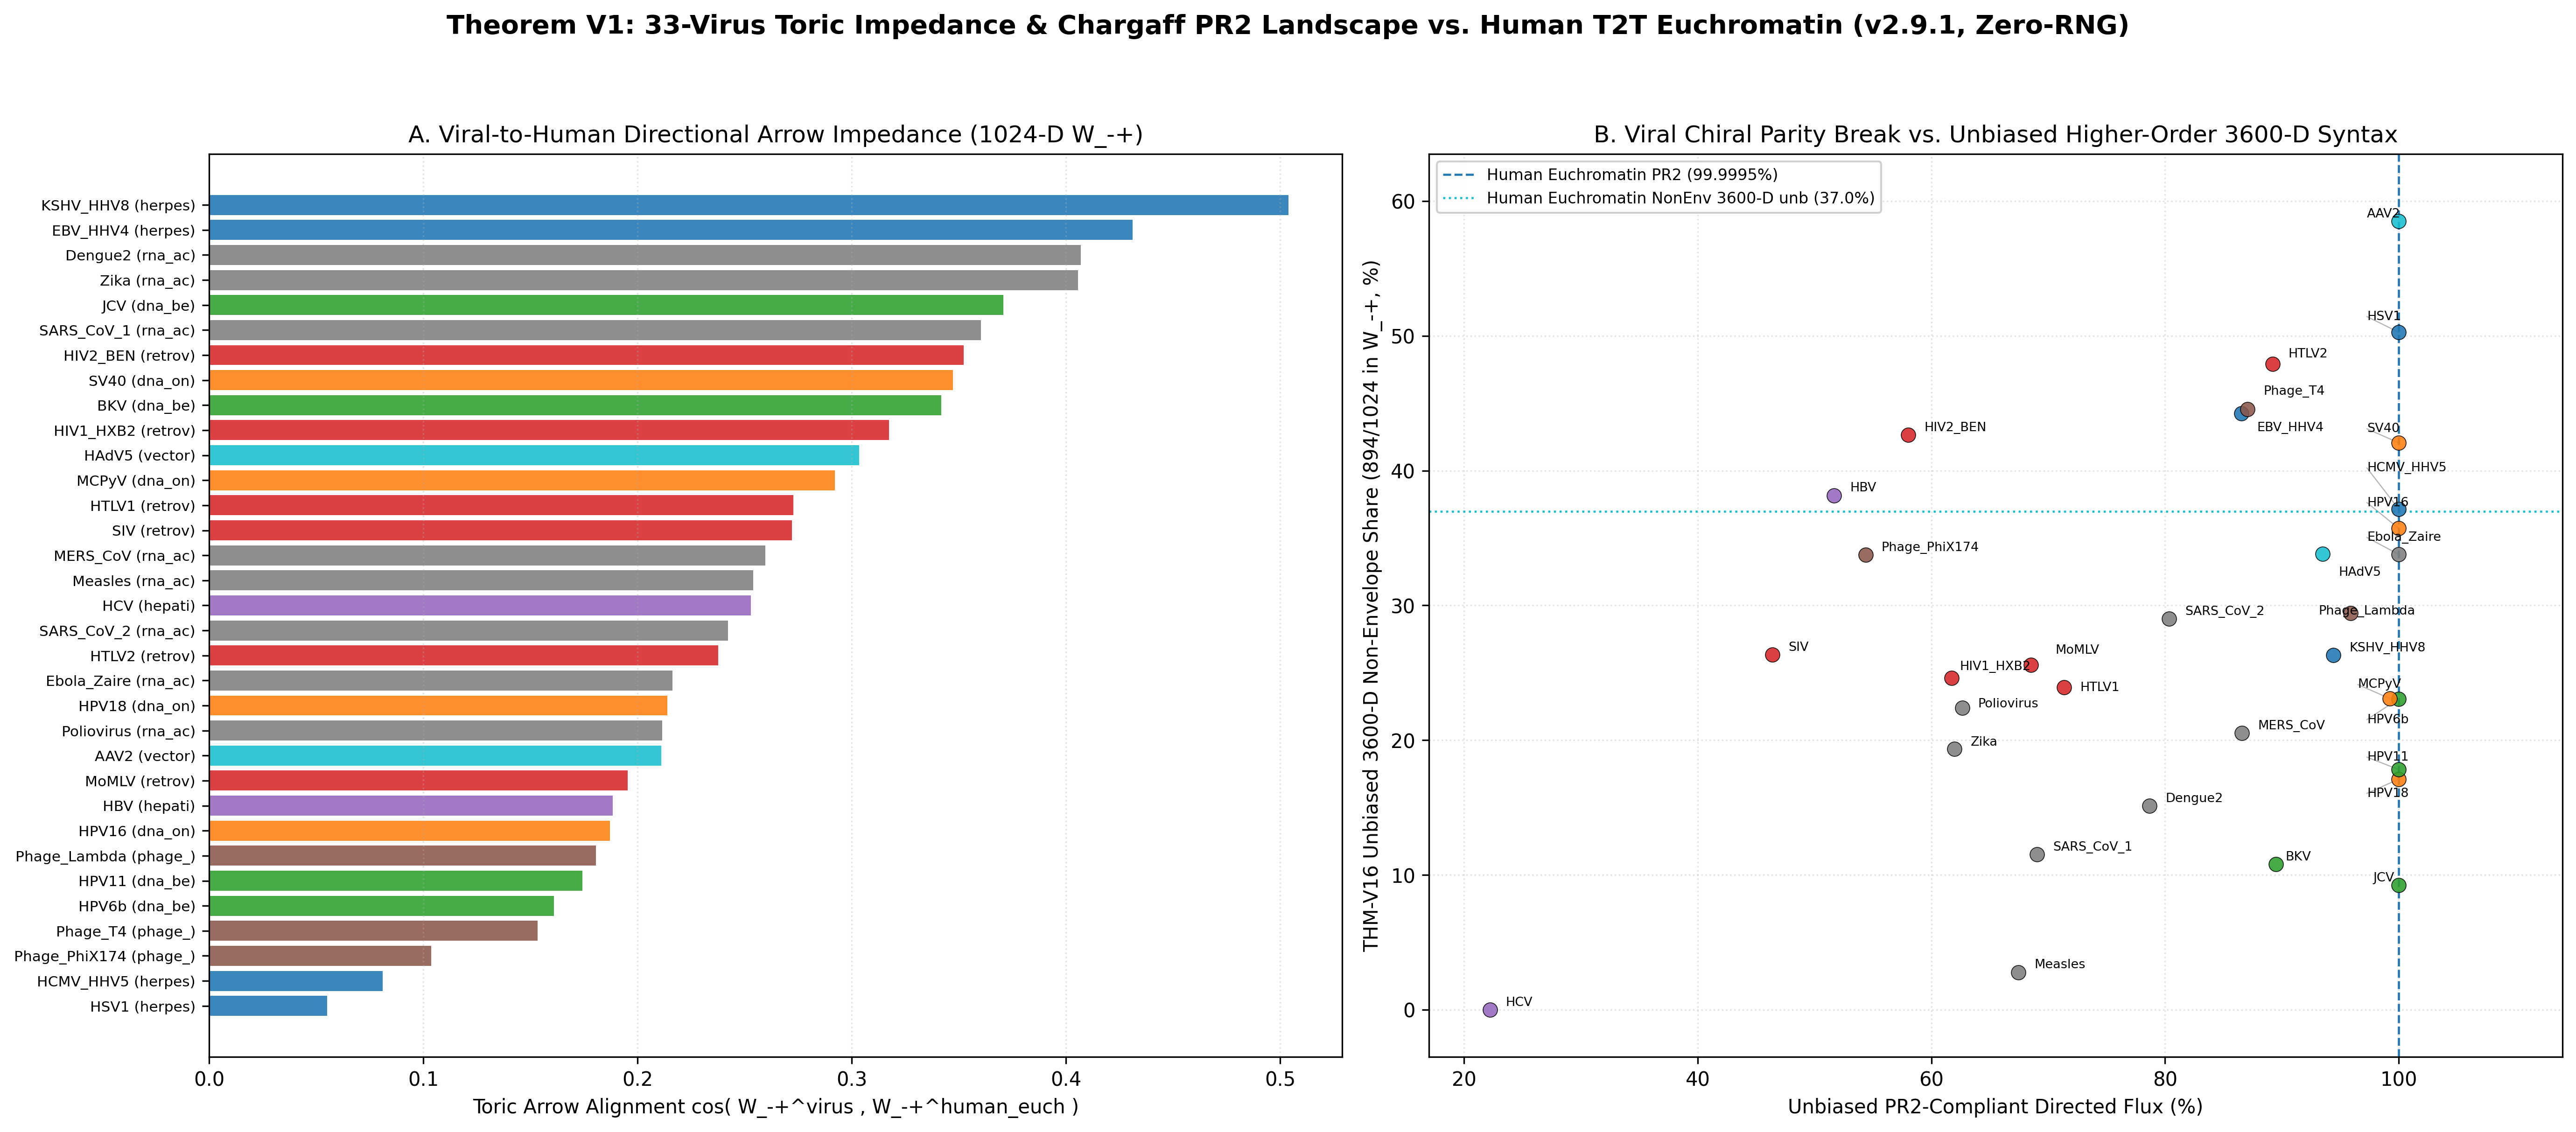
\includegraphics[width=0.96\textwidth]{fig_V1_virome_landscape}
\caption{Theorem~V1: 33-virus Klein $V_4$ toric impedance and Chargaff PR2 landscape versus the 24-chromosome human T2T-CHM13v2.0 euchromatin reference (\texttt{v2.9.1}). \textbf{(A)} Raw 1024-D directional arrow alignment $\cos(W_{-+}^{\text{virus}}, W_{-+}^{\text{human}})$. \textbf{(B)} Unbiased PR2-compliant directed flux share (\%) versus Theorem~V16 unbiased 3600-D non-envelope share (894/1024 dimensions inside $W_{-+}$, \%), showing human euchromatin baselines ($99.9995\%$ PR2-ok; $37.0\%$ unbiased non-envelope 3600-D).}
\label{fig:v1}
\end{figure}

\subsection{Multi-Lag Persistence Across Nucleosomal Scales (Theorem~V6)}

To determine whether viral directional syntax is confined to contiguous 6-mers ($d = 3\,\mathrm{bp}$) or persists across helical and nucleosomal spacings, Theorem~V6 profiles all 33 viral genomes across ten physical lags $d \in \{3, 6, 9, 10, 11, 15, 30, 90, 147, 171\}\,\mathrm{bp}$ (Table~\ref{tab:v6_multilag}; Figure~\ref{fig:v3}A).

\begin{table}[htbp]
\centering
\scriptsize
\setlength{\tabcolsep}{4.5pt}
\caption{Theorem~V6: Multi-lag unbiased toric flux $\|W_{-+}\|^2_{\mathrm{unb}}$, palindromic share at $d=6\,\mathrm{bp}$, and human euchromatin cosine alignment across $d \in \{3, 6, 30, 171\}\,\mathrm{bp}$ for all 33 viruses (\texttt{v2.9.1}).}
\label{tab:v6_multilag}
\fittable{%
\begin{tabular}{@{}llllll@{}}
\toprule
\textbf{Virus} & \textbf{Class} & \textbf{$d=3$ $\|W_{-+}\|^2_{\mathrm{unb}}$ ($\cos$)} & \textbf{$d=6$ $\|W_{-+}\|^2_{\mathrm{unb}}$ (Pal)} & \textbf{$d=30$ $\|W_{-+}\|^2_{\mathrm{unb}}$ ($\cos$)} & \textbf{$d=171$ $\|W_{-+}\|^2_{\mathrm{unb}}$ ($\cos$)} \\
\midrule
\texttt{HIV1\_HXB2}    & retro\_int  & $6.81\mathrm{e}{-6}$ ($+0.32$) & $-2.67\mathrm{e}{-7}$ (3.3\%) & $-1.79\mathrm{e}{-8}$ ($-0.00$) & $-2.43\mathrm{e}{-6}$ ($+0.00$) \\
\texttt{HIV2\_BEN}     & retro\_int  & $8.95\mathrm{e}{-6}$ ($+0.35$) &  $1.76\mathrm{e}{-6}$ (5.2\%) &  $5.92\mathrm{e}{-6}$ ($+0.06$) &  $2.93\mathrm{e}{-6}$ ($-0.03$) \\
\texttt{HTLV1}         & retro\_int  & $7.79\mathrm{e}{-6}$ ($+0.27$) &  $1.41\mathrm{e}{-6}$ (4.4\%) & $-8.63\mathrm{e}{-7}$ ($-0.01$) & $-2.34\mathrm{e}{-6}$ ($-0.01$) \\
\texttt{HTLV2}         & retro\_int  & $1.45\mathrm{e}{-5}$ ($+0.24$) &  $8.27\mathrm{e}{-6}$ (3.6\%) &  $4.53\mathrm{e}{-6}$ ($-0.02$) &  $3.98\mathrm{e}{-6}$ ($+0.03$) \\
\texttt{SIV}           & retro\_int  & $5.28\mathrm{e}{-6}$ ($+0.27$) &  $3.42\mathrm{e}{-6}$ (2.9\%) &  $3.40\mathrm{e}{-6}$ ($-0.02$) &  $1.65\mathrm{e}{-6}$ ($+0.04$) \\
\texttt{MoMLV}         & retro\_int  & $9.60\mathrm{e}{-6}$ ($+0.20$) &  $1.25\mathrm{e}{-6}$ (3.2\%) & $-1.26\mathrm{e}{-6}$ ($-0.01$) & $-1.77\mathrm{e}{-6}$ ($+0.02$) \\
\midrule
\texttt{HPV16}         & dna\_onco   & $1.05\mathrm{e}{-5}$ ($+0.19$) &  $1.60\mathrm{e}{-7}$ (2.6\%) & $-1.48\mathrm{e}{-6}$ ($-0.00$) & $-2.49\mathrm{e}{-6}$ ($-0.05$) \\
\texttt{HPV18}         & dna\_onco   & $1.45\mathrm{e}{-5}$ ($+0.21$) & $-2.26\mathrm{e}{-6}$ (4.1\%) & $-6.04\mathrm{e}{-7}$ ($+0.11$) & $-2.35\mathrm{e}{-6}$ ($-0.01$) \\
\texttt{HPV6b}         & dna\_benign & $1.17\mathrm{e}{-5}$ ($+0.16$) & $-9.47\mathrm{e}{-7}$ (3.4\%) &  $1.80\mathrm{e}{-6}$ ($+0.08$) & $-4.44\mathrm{e}{-7}$ ($-0.02$) \\
\texttt{HPV11}         & dna\_benign & $9.44\mathrm{e}{-6}$ ($+0.17$) & $-1.36\mathrm{e}{-6}$ (3.5\%) & $-2.51\mathrm{e}{-6}$ ($+0.07$) & $-1.50\mathrm{e}{-7}$ ($-0.02$) \\
\texttt{MCPyV}         & dna\_onco   & $1.32\mathrm{e}{-5}$ ($+0.29$) &  $1.09\mathrm{e}{-6}$ (6.0\%) & $-4.53\mathrm{e}{-7}$ ($+0.05$) &  $3.97\mathrm{e}{-6}$ ($+0.05$) \\
\texttt{SV40}          & dna\_onco   & $2.05\mathrm{e}{-5}$ ($+0.35$) & $-7.30\mathrm{e}{-7}$ (3.0\%) & $-7.37\mathrm{e}{-8}$ ($+0.01$) & $-3.54\mathrm{e}{-6}$ ($+0.04$) \\
\texttt{JCV}           & dna\_benign & $1.21\mathrm{e}{-5}$ ($+0.37$) & $-1.56\mathrm{e}{-6}$ (3.4\%) &  $4.14\mathrm{e}{-6}$ ($-0.01$) &  $1.20\mathrm{e}{-6}$ ($-0.03$) \\
\texttt{BKV}           & dna\_benign & $1.24\mathrm{e}{-5}$ ($+0.34$) & $-4.91\mathrm{e}{-7}$ (3.9\%) & $-3.03\mathrm{e}{-6}$ ($+0.03$) & $-2.82\mathrm{e}{-7}$ ($+0.05$) \\
\midrule
\texttt{HBV}           & hep\_hcc    & $9.27\mathrm{e}{-6}$ ($+0.19$) & $-5.51\mathrm{e}{-6}$ (3.9\%) & $-3.48\mathrm{e}{-6}$ ($-0.06$) & $-2.32\mathrm{e}{-6}$ ($+0.05$) \\
\texttt{HCV}           & hep\_hcc    & $7.05\mathrm{e}{-7}$ ($+0.25$) & $-1.22\mathrm{e}{-6}$ (4.0\%) & $-3.06\mathrm{e}{-6}$ ($+0.07$) &  $1.01\mathrm{e}{-6}$ ($+0.00$) \\
\midrule
\texttt{EBV\_HHV4}     & herpes\_lg  & $1.36\mathrm{e}{-5}$ ($+0.43$) &  $5.19\mathrm{e}{-6}$ (3.7\%) &  $1.65\mathrm{e}{-6}$ ($-0.01$) &  $1.89\mathrm{e}{-6}$ ($-0.04$) \\
\texttt{KSHV\_HHV8}    & herpes\_lg  & $5.36\mathrm{e}{-6}$ ($+0.50$) &  $1.07\mathrm{e}{-6}$ (4.3\%) &  $2.89\mathrm{e}{-7}$ ($+0.03$) &  $1.10\mathrm{e}{-7}$ ($-0.00$) \\
\texttt{HSV1}          & herpes\_lg  & $4.56\mathrm{e}{-6}$ ($+0.06$) &  $2.75\mathrm{e}{-6}$ (2.2\%) &  $5.63\mathrm{e}{-7}$ ($+0.08$) &  $3.67\mathrm{e}{-7}$ ($+0.02$) \\
\texttt{HCMV\_HHV5}    & herpes\_lg  & $6.00\mathrm{e}{-6}$ ($+0.08$) &  $1.16\mathrm{e}{-6}$ (5.1\%) &  $1.14\mathrm{e}{-7}$ ($+0.01$) &  $6.62\mathrm{e}{-8}$ ($-0.02$) \\
\texttt{AAV2}          & vec\_dna    & $1.15\mathrm{e}{-5}$ ($+0.21$) &  $6.21\mathrm{e}{-6}$ (3.8\%) &  $6.25\mathrm{e}{-7}$ ($+0.01$) &  $1.28\mathrm{e}{-6}$ ($+0.02$) \\
\texttt{HAdV5}         & vec\_dna    & $6.02\mathrm{e}{-6}$ ($+0.30$) &  $4.40\mathrm{e}{-7}$ (5.0\%) & $-2.00\mathrm{e}{-7}$ ($+0.05$) & $-2.09\mathrm{e}{-7}$ ($+0.01$) \\
\midrule
\texttt{SARS\_CoV\_2}  & rna\_acute  & $8.69\mathrm{e}{-6}$ ($+0.24$) &  $5.05\mathrm{e}{-7}$ (2.7\%) & $-3.62\mathrm{e}{-7}$ ($+0.04$) & $-7.43\mathrm{e}{-7}$ ($-0.04$) \\
\texttt{SARS\_CoV\_1}  & rna\_acute  & $6.02\mathrm{e}{-6}$ ($+0.36$) &  $1.24\mathrm{e}{-7}$ (3.9\%) &  $2.88\mathrm{e}{-7}$ ($-0.01$) & $-7.46\mathrm{e}{-7}$ ($-0.04$) \\
\texttt{MERS\_CoV}     & rna\_acute  & $4.18\mathrm{e}{-6}$ ($+0.26$) &  $4.96\mathrm{e}{-9}$ (4.2\%) & $-4.01\mathrm{e}{-7}$ ($+0.02$) &  $1.32\mathrm{e}{-7}$ ($+0.02$) \\
\texttt{Ebola\_Zaire}  & rna\_acute  & $4.82\mathrm{e}{-6}$ ($+0.22$) & $-1.05\mathrm{e}{-6}$ (2.5\%) & $-1.32\mathrm{e}{-6}$ ($+0.01$) & $-3.66\mathrm{e}{-7}$ ($+0.07$) \\
\texttt{Measles}       & rna\_acute  & $4.91\mathrm{e}{-6}$ ($+0.25$) &  $6.38\mathrm{e}{-7}$ (4.4\%) & $-1.27\mathrm{e}{-7}$ ($+0.01$) &  $5.60\mathrm{e}{-7}$ ($-0.03$) \\
\texttt{Poliovirus}    & rna\_acute  & $7.58\mathrm{e}{-6}$ ($+0.21$) & $-9.96\mathrm{e}{-7}$ (3.6\%) &  $2.89\mathrm{e}{-6}$ ($-0.00$) & $-3.79\mathrm{e}{-7}$ ($-0.07$) \\
\texttt{Zika}          & rna\_acute  & $1.23\mathrm{e}{-5}$ ($+0.41$) & $-6.15\mathrm{e}{-7}$ (4.1\%) & $-6.52\mathrm{e}{-7}$ ($-0.01$) &  $2.93\mathrm{e}{-7}$ ($+0.01$) \\
\texttt{Dengue2}       & rna\_acute  & $1.31\mathrm{e}{-5}$ ($+0.41$) &  $1.06\mathrm{e}{-6}$ (2.4\%) & $-1.55\mathrm{e}{-6}$ ($-0.06$) & $-5.71\mathrm{e}{-7}$ ($-0.00$) \\
\midrule
\texttt{Phage\_Lambda} & phage       & $1.54\mathrm{e}{-5}$ ($+0.18$) &  $5.60\mathrm{e}{-7}$ (3.0\%) &  $8.83\mathrm{e}{-8}$ ($+0.01$) &  $2.29\mathrm{e}{-8}$ ($+0.06$) \\
\texttt{Phage\_T4}     & phage       & $9.69\mathrm{e}{-6}$ ($+0.15$) &  $1.25\mathrm{e}{-6}$ (4.6\%) & $-5.73\mathrm{e}{-8}$ ($-0.02$) & $-2.10\mathrm{e}{-8}$ ($+0.03$) \\
\texttt{Phage\_PhiX174}& phage       & $9.48\mathrm{e}{-6}$ ($+0.10$) &  $7.78\mathrm{e}{-7}$ (3.7\%) & $-6.44\mathrm{e}{-6}$ ($-0.02$) & $-1.93\mathrm{e}{-6}$ ($-0.01$) \\
\bottomrule
\end{tabular}
}
\end{table}

Across most compact RNA and small DNA viruses, unbiased directional flux $\|W_{-+}\|^2_{\mathrm{unb}}$ collapses rapidly by $d = 6\text{--}30\,\mathrm{bp}$ (with transient helical-turn revivals at $d = 10\text{--}11\,\mathrm{bp}$ driven by coding periodicity; Figure~\ref{fig:v3}A). By contrast, all four large chromatin-forming herpesviruses maintain strictly positive unbiased flux through $d = 171\,\mathrm{bp}$ (\texttt{EBV\_HHV4}: $1.36 \times 10^{-5} \to 5.19 \times 10^{-6} \to 1.65 \times 10^{-6} \to 1.89 \times 10^{-6}$; \texttt{HSV1}: $4.56 \times 10^{-6} \to 3.67 \times 10^{-7}$; \texttt{KSHV\_HHV8}: $5.36 \times 10^{-6} \to 1.10 \times 10^{-7}$), alongside the long-range tandem/repeat architecture of \texttt{AAV2} and retroviruses \texttt{HTLV2}/\texttt{HIV2\_BEN}. Notably, cross-species alignment to the human euchromatin arrow is strictly concentrated at the adjacent hexamer scale ($d = 3\,\mathrm{bp}$), dropping near zero at $d \ge 30\,\mathrm{bp}$.

\subsection{Beyond-Markov-1 and Beyond-Markov-2 Viral Mimicry (Theorems~V9, V11, V11.2 \& V11.3)}

To test whether viral alignment to human euchromatin is an artifact of dinucleotide (Markov-1) or 64-trinucleotide (Markov-2) composition, we compute the exact linear probability-excess residuals $w^{\perp M1}$ and $w^{\perp M2}$ (alongside Gram--Schmidt orthogonal projections as sensitivity controls) across all 33 viruses (Table~\ref{tab:v11_all33}; Figure~\ref{fig:v7}A).

\begin{table}[htbp]
\centering
\scriptsize
\setlength{\tabcolsep}{4.5pt}
\caption{Theorems~V11 \& V11.2: Nested compositional decomposition of viral-to-human directional alignment across all 33 viruses, ranked by Beyond-Markov-2 (64-trinucleotide-controlled) cosine similarity (\texttt{v2.9.1}).}
\label{tab:v11_all33}
\fittable{%
\begin{tabular}{@{}llrrrrrrrr@{}}
\toprule
\textbf{Virus} & \textbf{Class} & \textbf{GC\%} & \textbf{Total 1024-D} & \textbf{3600-D} & \textbf{CpG-Free} & \textbf{3600-D CpG-fr} & \textbf{Beyond-M1} & \textbf{Beyond-M2} & \textbf{$\cos(\text{Self}, M2)$} \\
\midrule
\texttt{KSHV\_HHV8}    & herpes\_lg  & 53.8 & $+0.504$ & $+0.170$ & $+0.507$ & $+0.146$ & $+0.333$ & $\mathbf{+0.232}$ & $+0.700$ \\
\texttt{EBV\_HHV4}     & herpes\_lg  & 59.5 & $+0.431$ & $+0.063$ & $+0.431$ & $+0.054$ & $+0.223$ & $\mathbf{+0.165}$ & $+0.696$ \\
\texttt{HCMV\_HHV5}    & herpes\_lg  & 57.5 & $+0.081$ & $+0.058$ & $+0.151$ & $+0.029$ & $+0.217$ & $\mathbf{+0.146}$ & $+0.685$ \\
\texttt{HAdV5}         & vec\_dna    & 55.2 & $+0.303$ & $+0.096$ & $+0.343$ & $+0.081$ & $+0.195$ & $\mathbf{+0.140}$ & $+0.559$ \\
\texttt{HSV1}          & herpes\_lg  & 68.3 & $+0.055$ & $+0.035$ & $+0.079$ & $+0.032$ & $+0.151$ & $\mathbf{+0.127}$ & $+0.540$ \\
\texttt{Phage\_Lambda} & phage       & 49.9 & $+0.181$ & $+0.038$ & $+0.218$ & $+0.053$ & $+0.217$ & $\mathbf{+0.105}$ & $+0.697$ \\
\texttt{HPV16}         & dna\_onco   & 36.5 & $+0.187$ & $+0.085$ & $+0.171$ & $+0.079$ & $+0.140$ & $\mathbf{+0.092}$ & $+0.443$ \\
\texttt{AAV2}          & vec\_dna    & 53.8 & $+0.211$ & $+0.065$ & $+0.216$ & $+0.060$ & $+0.079$ & $\mathbf{+0.089}$ & $+0.289$ \\
\texttt{HIV2\_BEN}     & retro\_int  & 45.7 & $+0.352$ & $+0.131$ & $+0.326$ & $+0.112$ & $+0.161$ & $\mathbf{+0.088}$ & $+0.409$ \\
\texttt{HTLV2}         & retro\_int  & 53.8 & $+0.238$ & $+0.046$ & $+0.215$ & $+0.035$ & $+0.134$ & $\mathbf{+0.087}$ & $+0.386$ \\
\texttt{Poliovirus}    & rna\_acute  & 46.3 & $+0.212$ & $+0.032$ & $+0.193$ & $+0.024$ & $+0.062$ & $\mathbf{+0.077}$ & $+0.359$ \\
\texttt{BKV}           & dna\_benign & 39.5 & $+0.342$ & $+0.102$ & $+0.319$ & $+0.051$ & $+0.163$ & $\mathbf{+0.072}$ & $+0.475$ \\
\texttt{HCV}           & hep\_hcc    & 58.2 & $+0.253$ & $+0.042$ & $+0.245$ & $+0.050$ & $+0.094$ & $\mathbf{+0.072}$ & $+0.312$ \\
\texttt{HTLV1}         & retro\_int  & 53.5 & $+0.273$ & $+0.062$ & $+0.255$ & $+0.044$ & $+0.150$ & $\mathbf{+0.069}$ & $+0.442$ \\
\texttt{SV40}          & dna\_onco   & 40.8 & $+0.347$ & $+0.130$ & $+0.335$ & $+0.100$ & $+0.160$ & $\mathbf{+0.059}$ & $+0.496$ \\
\texttt{HPV11}         & dna\_benign & 41.0 & $+0.174$ & $+0.038$ & $+0.154$ & $+0.031$ & $+0.082$ & $\mathbf{+0.055}$ & $+0.491$ \\
\texttt{HPV18}         & dna\_onco   & 40.4 & $+0.214$ & $+0.092$ & $+0.202$ & $+0.083$ & $+0.143$ & $\mathbf{+0.055}$ & $+0.525$ \\
\texttt{JCV}           & dna\_benign & 40.4 & $+0.371$ & $+0.101$ & $+0.341$ & $+0.051$ & $+0.139$ & $\mathbf{+0.052}$ & $+0.522$ \\
\texttt{HPV6b}         & dna\_benign & 40.9 & $+0.161$ & $+0.020$ & $+0.143$ & $+0.013$ & $+0.062$ & $\mathbf{+0.046}$ & $+0.487$ \\
\texttt{Dengue2}       & rna\_acute  & 45.8 & $+0.407$ & $+0.126$ & $+0.388$ & $+0.088$ & $+0.172$ & $\mathbf{+0.036}$ & $+0.590$ \\
\texttt{HBV}           & hep\_hcc    & 48.5 & $+0.188$ & $+0.023$ & $+0.180$ & $+0.010$ & $+0.049$ & $\mathbf{+0.029}$ & $+0.324$ \\
\texttt{Zika}          & rna\_acute  & 50.9 & $+0.406$ & $+0.096$ & $+0.377$ & $+0.051$ & $+0.116$ & $\mathbf{+0.028}$ & $+0.574$ \\
\texttt{MoMLV}         & retro\_int  & 53.0 & $+0.195$ & $-0.011$ & $+0.158$ & $-0.030$ & $-0.040$ & $\mathbf{+0.025}$ & $+0.437$ \\
\texttt{MCPyV}         & dna\_onco   & 40.7 & $+0.292$ & $+0.067$ & $+0.258$ & $+0.023$ & $+0.098$ & $\mathbf{+0.020}$ & $+0.444$ \\
\texttt{Phage\_PhiX174}& phage       & 44.8 & $+0.104$ & $+0.074$ & $+0.125$ & $+0.081$ & $+0.035$ & $\mathbf{+0.018}$ & $+0.342$ \\
\texttt{Ebola\_Zaire}  & rna\_acute  & 41.1 & $+0.216$ & $+0.036$ & $+0.200$ & $+0.013$ & $-0.006$ & $\mathbf{-0.007}$ & $+0.422$ \\
\texttt{SIV}           & retro\_int  & 44.4 & $+0.272$ & $+0.059$ & $+0.254$ & $+0.048$ & $+0.086$ & $\mathbf{-0.014}$ & $+0.429$ \\
\texttt{Measles}       & rna\_acute  & 47.4 & $+0.254$ & $+0.017$ & $+0.213$ & $-0.013$ & $-0.039$ & $\mathbf{-0.019}$ & $+0.521$ \\
\texttt{HIV1\_HXB2}    & retro\_int  & 42.1 & $+0.317$ & $+0.075$ & $+0.285$ & $+0.040$ & $+0.084$ & $\mathbf{-0.020}$ & $+0.461$ \\
\texttt{Phage\_T4}     & phage       & 35.3 & $+0.153$ & $-0.008$ & $+0.177$ & $-0.019$ & $+0.073$ & $\mathbf{-0.029}$ & $+0.596$ \\
\texttt{SARS\_CoV\_1}  & rna\_acute  & 40.8 & $+0.360$ & $+0.069$ & $+0.333$ & $+0.035$ & $+0.060$ & $\mathbf{-0.029}$ & $+0.623$ \\
\texttt{MERS\_CoV}     & rna\_acute  & 41.2 & $+0.260$ & $+0.044$ & $+0.240$ & $+0.017$ & $+0.009$ & $\mathbf{-0.048}$ & $+0.505$ \\
\texttt{SARS\_CoV\_2}  & rna\_acute  & 38.0 & $+0.242$ & $-0.012$ & $+0.205$ & $-0.041$ & $-0.021$ & $\mathbf{-0.079}$ & $+0.592$ \\
\bottomrule
\end{tabular}
}
\end{table}

Table~\ref{tab:v11_all33} reveals a striking inversion once low-order composition is projected out:
\begin{itemize}
    \item \textbf{Unmasking nuclear dsDNA mimicry:} All five largest nuclear dsDNA viruses rise immediately to the top five ranks of Beyond-Markov-2 alignment: \texttt{KSHV\_HHV8} ($+0.232$), \texttt{EBV\_HHV4} ($+0.165$), \texttt{HCMV\_HHV5} ($+0.146$), \texttt{HAdV5} ($+0.140$), and \texttt{HSV1} ($+0.127$). Remarkably, \texttt{HCMV\_HHV5} and \texttt{HSV1}---which looked deceptively weak in raw 1024-D space ($+0.081$ and $+0.055$) because their high GC content ($57.5\%$ and $68.3\%$) shifts low-order codon marginals away from $41\%$ GC human euchromatin---jump to Ranks~3 and~5 once their own 64-trinucleotide Markov-2 background is removed.
    \item \textbf{Collapse of cytoplasmic RNA viruses:} Conversely, the high raw scores of cytoplasmic RNA flaviviruses (\texttt{Dengue2} $+0.407 \to +0.036$; \texttt{Zika} $+0.406 \to +0.028$) and betacoronaviruses (\texttt{SARS\_CoV\_1} $+0.360 \to -0.029$; \texttt{MERS\_CoV} $+0.260 \to -0.048$; \texttt{SARS\_CoV\_2} $+0.242 \to -0.079$) collapse completely once Markov-2 expectations are subtracted, proving that their raw $W_{-+}$ resemblance was driven by low-order dinucleotide/trinucleotide composition rather than genuine higher-order 6-mer syntax.
    \item \textbf{Independent confirmation at low GC and small size:} Compact, AT-rich \texttt{HPV16} ($36.5\%$ GC, $7.9\,\mathrm{kb}$) retains strong positive Beyond-Markov-2 alignment ($+0.092$, Rank~7), demonstrating that nuclear euchromatic hexamer mimicry does not require high GC content or a large genome. Among bacteriophages, the temperate integrating \texttt{Phage\_Lambda} ($+0.105$) contrasts sharply with lytic \texttt{Phage\_T4} ($-0.029$).
\end{itemize}

Because Spearman rank correlation across the 33 viruses shows a residual association between $\mathrm{GC}\%$ and Beyond-Markov-2 alignment ($\rho_S = +0.559$, $p = 7.11 \times 10^{-4}$; whereas $\mathrm{GC}\%$ vs.\ Total 1024-D is null at $\rho_S = -0.005$, $p = 0.979$), a rigorous red-team test must control simultaneously for $\mathrm{GC}\%$ and genome length $\log_{10}(L)$. Table~\ref{tab:v9_viral} and Theorem~\ref{thm:v11_3} document the exact Zero-RNG nonparametric Mann--Whitney tests (computed by exact dynamic programming, verified to error $0.0$ in \texttt{thmV9\_exact\_mann\_whitney\_dp\_err}).

\begin{table}[htbp]
\centering
\scriptsize
\setlength{\tabcolsep}{3.8pt}
\caption{Theorems~V9, V11.3 \& V18: Exact Zero-RNG Mann--Whitney viral group discrimination before and after simultaneous OLS covariate residualization for $\mathrm{GC}\%$, $\log_{10}(L)$, and ZAP $\mathrm{CpG\ O/E}$, with discrete minimum $p_{\min} = 2/\binom{n_1+n_2}{n_1}$ and global Benjamini--Hochberg $q_{\mathrm{BH}}$ across all $m = 50$ audit tests (\texttt{v2.9.1}). Phage separation in raw 1024-D is purely compositional (null beyond Markov-2).}
\label{tab:v9_viral}
\fittable{%
\begin{tabular}{@{}llrcrrrr@{}}
\toprule
\textbf{Viral Group Contrast} & \textbf{Metric} & \textbf{$n_1 / n_2$} & \textbf{Median 1 vs.\ Median 2} & \textbf{$r_{\mathrm{rb}}$} & \textbf{Two-Sided $p$} & \textbf{$p_{\min}$} & \textbf{$q_{\mathrm{BH}}$} \\
\midrule
Onco/Integrating vs.\ Acute RNA & Total 1024-D $\cos W_{-+}$ & 18 / 8 & $+0.2625$ vs.\ $+0.2568$ & $-0.208$ & $4.29\times 10^{-1}$ & $1.28\times 10^{-6}$ & 0.6912 \\
Onco/Integrating vs.\ Acute RNA & De-attenuated $\cos_{\mathrm{unb}}$ ($z\ge 3$) & 16 / 8 & $+0.4763$ vs.\ $+0.5056$ & $-0.109$ & $6.97\times 10^{-1}$ & $2.72\times 10^{-6}$ & 0.8933 \\
Onco/Integrating vs.\ Acute RNA & 3600-D $\cos W_{-+}$ & 18 / 8 & $+0.0642$ vs.\ $+0.0402$ & $+0.306$ & $2.38\times 10^{-1}$ & $1.28\times 10^{-6}$ & 0.4574 \\
Onco/Integrating vs.\ Acute RNA & Beyond-M1 (Dinuc) & 18 / 8 & $+0.1415$ vs.\ $+0.0344$ & $+0.597$ & $1.58\times 10^{-2}$ & $1.28\times 10^{-6}$ & 0.0608 \\
Onco/Integrating vs.\ Acute RNA & Beyond-M2 (Trinuc) & 18 / 8 & $+0.0796$ vs.\ $-0.0133$ & $+0.708$ & $3.35\times 10^{-3}$ & $1.28\times 10^{-6}$ & 0.0335 \\
Onco/Integrating vs.\ Acute RNA & Beyond-M2 (OLS GC+$\log_{10}L$) & 18 / 8 & $+0.0164$ vs.\ $-0.0434$ & $+0.597$ & $1.58\times 10^{-2}$ & $1.28\times 10^{-6}$ & 0.0608 \\
Onco/Integrating vs.\ Acute RNA & Beyond-M2 (OLS GC+$\log_{10}L$+CpG) & 18 / 8 & $+0.0105$ vs.\ $-0.0427$ & $+0.639$ & $9.23\times 10^{-3}$ & $1.28\times 10^{-6}$ & 0.0512 \\
\midrule
\textbf{Nuclear DNA vs.\ Acute RNA (Primary)} & \textbf{Beyond-M2 (OLS GC+$\log_{10}L$)} & \textbf{14 / 8} & $\mathbf{+0.0271}$ \textbf{vs.}\ $\mathbf{-0.0570}$ & $\mathbf{+0.893}$ & \textbf{$1.88\times 10^{-4}$} & $6.25\times 10^{-6}$ & \textbf{0.0031} \\
\textbf{Nuclear DNA vs.\ Acute RNA (ZAP Ctrl)} & \textbf{Beyond-M2 (OLS GC+$\log_{10}L$+CpG)} & \textbf{14 / 8} & $\mathbf{+0.0268}$ \textbf{vs.}\ $\mathbf{-0.0567}$ & $\mathbf{+0.893}$ & \textbf{$1.88\times 10^{-4}$} & $6.25\times 10^{-6}$ & \textbf{0.0031} \\
Nuclear DNA vs.\ Acute RNA (GS Ctrl) & Beyond-M2 GS (OLS GC+$\log_{10}L$) & 14 / 8 & $+0.0196$ vs.\ $-0.0275$ & $+0.679$ & $8.12\times 10^{-3}$ & $6.25\times 10^{-6}$ & 0.0508 \\
Nuclear DNA vs.\ Acute RNA (GS+ZAP) & Beyond-M2 GS (OLS GC+$\log_{10}L$+CpG) & 14 / 8 & $+0.0194$ vs.\ $-0.0274$ & $+0.696$ & $6.37\times 10^{-3}$ & $6.25\times 10^{-6}$ & 0.0508 \\
\midrule
High-Risk DNA Onco vs.\ Benign & Beyond-M2 (Trinuc) & 4 / 4 & $+0.0567$ vs.\ $+0.0533$ & $+0.125$ & $8.86\times 10^{-1}$ & $2.86\times 10^{-2}$ & 0.9627 \\
Human Viruses vs.\ Phages (raw comp.) & Total 1024-D $\cos W_{-+}$ & 30 / 3 & $+0.2568$ vs.\ $+0.1534$ & $+0.822$ & $1.50\times 10^{-2}$ & $3.67\times 10^{-4}$ & 0.0608 \\
Human Viruses vs.\ Phages (M2-ctrl) & Beyond-M2 (Trinuc) & 30 / 3 & $+0.0547$ vs.\ $+0.0180$ & $+0.222$ & $5.71\times 10^{-1}$ & $3.67\times 10^{-4}$ & 0.7937 \\
\bottomrule
\end{tabular}
}
\end{table}

\begin{theorem}[Covariate-Controlled Beyond-Markov-2 Nuclear dsDNA Mimicry; THM-V11.3]
\label{thm:v11_3}
Across the 33-virus cohort of frozen release \texttt{v2.9.1}:
\begin{enumerate}
    \item \textbf{Null length confounding:} Genome length $\log_{10}(L)$ exhibits no significant rank correlation with Beyond-Markov-2 human alignment:
    \begin{equation}
        \rho_S\bigl(\log_{10} L,\; \cos W_{-+}^{\perp M2}\bigr) = +0.103, \qquad p = 0.570.
    \end{equation}
    \item \textbf{Survival of Oncogenic/Integrating vs.\ Acute RNA separation:} While unadjusted Total 1024-D cosine shows no discrimination ($p = 0.429$), projecting out Markov-1 ($p = 1.58 \times 10^{-2}$) and Markov-2 ($r_{\mathrm{rb}} = +0.708$, $p = 3.35 \times 10^{-3}$) exposes strong separation that survives simultaneous OLS residualization against $\mathrm{GC}\%$ and $\log_{10}(L)$ ($n = 18/8$, median residual $+0.0164$ vs.\ $-0.0434$, $r_{\mathrm{rb}} = +0.597$, $p = 1.58 \times 10^{-2}$).
    \item \textbf{Near-complete Nuclear DNA vs.\ Acute Cytoplasmic RNA separation (ZAP-, AAV2-, and FDR-controlled):} Restricting to nuclear DNA viruses ($n = 14$, comprising 13 dsDNA viruses plus the nuclear-replicating ssDNA parvovirus \texttt{AAV2}, which persists as nuclear dsDNA episomes) versus acute cytoplasmic RNA controls ($n = 8$) under simultaneous control for all 64 trinucleotides, $\mathrm{GC}\%$, and $\log_{10}(L)$ yields near-total separation that remains unchanged upon adding ZAP $\mathrm{CpG\ O/E}$ as a third OLS covariate and survives global Benjamini--Hochberg correction across all $m = 50$ audit tests ($n_{\mathrm{sig}} = 5$ at $q_{\mathrm{BH}} \le 0.05$):
    \begin{equation}
    \begin{aligned}
        &\text{median residual } +0.0271 \text{ vs.\ } -0.0570\;\;(\text{3-cov: } +0.0268 \text{ vs.\ } -0.0567), \\
        &\qquad r_{\mathrm{rb}} = +0.893, \qquad p = 1.88 \times 10^{-4}, \qquad q_{\mathrm{BH}} = 0.0031.
    \end{aligned}
    \end{equation}
    Excluding the ssDNA parvovirus \texttt{AAV2} to retain strictly double-stranded nuclear DNA genomes ($n = 13/8$) slightly strengthens the separation under both 2-covariate OLS ($r_{\mathrm{rb}} = +0.904$, $p = 1.87 \times 10^{-4}$) and 3-covariate ZAP-adjusted OLS ($r_{\mathrm{rb}} = +0.904$, $p = 1.87 \times 10^{-4}$). Replacing the linear probability-excess residual by the Gram--Schmidt orthogonal projection confirms robustness under both 2-covariate ($r_{\mathrm{rb}} = +0.679$, $p = 8.12 \times 10^{-3}$) and 3-covariate ZAP-adjusted OLS ($r_{\mathrm{rb}} = +0.696$, $p = 6.37 \times 10^{-3}$, $q_{\mathrm{BH}} = 0.0508$; Table~\ref{tab:v9_viral}).
\end{enumerate}
\end{theorem}

Importantly, high-risk DNA oncoviruses ($n = 4$) do not differ from their benign DNA viral counterparts ($n = 4$; $p = 0.886$), proving that Beyond-Markov-2 mimicry is a general property of \emph{nuclear chromatin residence} rather than oncogenicity per se.

\subsection{Exact Klein-Orbit 6-mer Motif Attribution in Nuclear Herpesviruses (Theorem~V13A--C)}

To rule out the possibility that nuclear dsDNA mimicry is driven merely by CpG-containing motifs, Theorem~V13 decomposes the inner product $\langle W_{-+}^{\text{virus}}, W_{-+}^{\text{human}} \rangle_F$ into exact additive $V_4$-orbits (Table~\ref{tab:v13_viral_orbits}).

\begin{table}[htbp]
\centering
\scriptsize
\setlength{\tabcolsep}{4.0pt}
\caption{Theorem~V13A--C: Top-8 exact Klein $V_4$-orbit 6-mer contributors to viral-to-human euchromatic alignment in \texttt{KSHV\_HHV8} (Total 1024-D and Beyond-Markov-2 residual) and \texttt{EBV\_HHV4} (Beyond-Markov-2 residual), verified to orbit-sum error $2.84 \times 10^{-14}$ (\texttt{v2.9.1}).}
\label{tab:v13_viral_orbits}
\fittable{%
\begin{tabular}{@{}r l l r c | l l r c | l l r c@{}}
\toprule
 & \multicolumn{4}{c|}{\textbf{13A: \texttt{KSHV} Total 1024-D}} & \multicolumn{4}{c|}{\textbf{13B: \texttt{KSHV} Beyond-M2}} & \multicolumn{4}{c}{\textbf{13C: \texttt{EBV} Beyond-M2}} \\
\textbf{\#} & \textbf{6-mer} & \textbf{Mirror} & \textbf{Share} & \textbf{CpG} & \textbf{6-mer} & \textbf{Mirror} & \textbf{Share} & \textbf{CpG} & \textbf{6-mer} & \textbf{Mirror} & \textbf{Share} & \textbf{CpG} \\
\midrule
1 & \texttt{CCC-AGG} & \texttt{CCT-GGG} & $+2.81\%$ & No & \texttt{CCC-AGG} & \texttt{CCT-GGG} & $+4.69\%$ & No & \texttt{GCC-TCC} & \texttt{GGA-GGC} & $+6.13\%$ & No \\
2 & \texttt{GAA-AAC} & \texttt{GTT-TTC} & $+2.32\%$ & No & \texttt{AAA-CAA} & \texttt{TTG-TTT} & $+3.41\%$ & No & \texttt{CCA-GCC} & \texttt{GGC-TGG} & $+5.43\%$ & No \\
3 & \texttt{CCA-GGA} & \texttt{TCC-TGG} & $+2.16\%$ & No & \texttt{AGC-TGG} & \texttt{CCA-GCT} & $+3.31\%$ & No & \texttt{GCC-ACC} & \texttt{GGT-GGC} & $+5.31\%$ & No \\
4 & \texttt{GCC-ACC} & \texttt{GGT-GGC} & $+1.88\%$ & No & \texttt{TTT-ATT} & \texttt{AAT-AAA} & $+2.97\%$ & No & \texttt{CCA-GGC} & \texttt{GCC-TGG} & $+5.00\%$ & No \\
5 & \texttt{CAG-GAG} & \texttt{CTC-CTG} & $+1.81\%$ & No & \texttt{CCT-CCC} & \texttt{GGG-AGG} & $+2.82\%$ & No & \texttt{AAA-GAA} & \texttt{TTC-TTT} & $+4.74\%$ & No \\
6 & \texttt{GGA-GGC} & \texttt{GCC-TCC} & $+1.52\%$ & No & \texttt{CCA-GGA} & \texttt{TCC-TGG} & $+2.69\%$ & No & \texttt{CCC-GGG} & \texttt{CCC-GGG} & $+4.62\%$ & Yes \\
7 & \texttt{GCC-AGG} & \texttt{CCT-GGC} & $+1.42\%$ & No & \texttt{GCC-AGG} & \texttt{CCT-GGC} & $+2.47\%$ & No & \texttt{GCC-GGG} & \texttt{CCC-GGC} & $+3.61\%$ & Yes \\
8 & \texttt{GGC-AGC} & \texttt{GCT-GCC} & $+1.34\%$ & No & \texttt{CAG-GAG} & \texttt{CTC-CTG} & $+2.31\%$ & No & \texttt{CTC-CTG} & \texttt{CAG-GAG} & $+3.56\%$ & No \\
\bottomrule
\end{tabular}
}
\end{table}

In \texttt{KSHV\_HHV8}, all eight leading orbits in both Total 1024-D ($15.26\%$ cumulative weight) and Beyond-Markov-2 ($24.67\%$ cumulative weight) are $100\%$ CpG-free, led in both channels by the size-4 mirror orbit \texttt{CCC-AGG} / \texttt{CCT-GGG} ($+2.81\%$ total, $+4.69\%$ Beyond-M2) and purine/pyrimidine-tract junctions (\texttt{AAA-CAA}, \texttt{TTT-ATT}, \texttt{CCA-GGA}, \texttt{CAG-GAG}). In \texttt{EBV\_HHV4}, the top eight Beyond-M2 orbits account for $38.40\%$ of the entire orthogonal inner product, with six of eight strictly CpG-free (led by \texttt{GCC-TCC} / \texttt{GGA-GGC} at $+6.13\%$) and the self-mirror size-2 orbit \texttt{CCC-GGG} entering only at Rank~6 ($+4.62\%$). Together, Tables~\ref{tab:v11_all33}--\ref{tab:v13_viral_orbits} establish that nuclear dsDNA viruses faithfully encode higher-order, CpG-independent directional hexamer syntax of human euchromatin.

%==============================================================================
\section{Evolutionary APOBEC3 Versus ZAP/CpG Evasion Dichotomy}
\label{sec:evasion}
%==============================================================================

Human innate immunity restricts viral genomes through at least two sequence-specific nucleic-acid effectors operating on distinct motifs: the zinc-finger antiviral protein (ZAP), which binds $\mathrm{CpG}$ dinucleotides in viral RNA, and the APOBEC3 family of cytidine deaminases, which edit cytosines within single-stranded $\mathrm{TCW}$ ($\mathrm{TCA}/\mathrm{TCT}$) motifs. To disentangle genuine evolutionary motif purging from passive GC-content variation, Theorems~V10 and V10.2 evaluate both mononucleotide-normalized $\mathrm{TCW\ O/E}$ (Base), dinucleotide-normalized $\mathrm{TCW\ O/E}$ (Dinuc), and $\mathrm{CpG\ O/E}$ alongside exact unbiased \textit{de novo} APOBEC3 \texttt{SBS2(+)} chiral susceptibility $\chi_{--}^{\mathrm{de\,novo,unb}} \times 10^4$ across all 33 viral genomes (Table~\ref{tab:v10_all33}; Figure~\ref{fig:v6}).

\begin{table}[htbp]
\centering
\scriptsize
\setlength{\tabcolsep}{4.5pt}
\caption{Theorems~V10 \& V10.2: GC- and dinucleotide-controlled viral APOBEC3 $\mathrm{TCW}$ motif evasion versus ZAP $\mathrm{CpG}$ suppression and unbiased \textit{de novo} \texttt{SBS2(+)} chiral susceptibility across all 33 RefSeq viruses (\texttt{v2.9.1}).}
\label{tab:v10_all33}
\fittable{%
\begin{tabular}{@{}llrrrrrrr@{}}
\toprule
\textbf{Virus} & \textbf{Class} & \textbf{GC\%} & \textbf{TCW\%} & \textbf{TCW O/E (Base)} & \textbf{TCW O/E (Dinuc)} & \textbf{CpG O/E} & \textbf{SBS2(+) Chiral\%} & \textbf{De Novo $\chi_{--}^{\mathrm{unb}}\!\times\!10^4$} \\
\midrule
\texttt{HIV1\_HXB2}    & retro\_int  & 42.1 & 2.42 & $\mathbf{1.053}$ & 0.981 & 0.206 & 45.74\% & 0.085 \\
\texttt{HIV2\_BEN}     & retro\_int  & 45.7 & 2.40 & $\mathbf{1.045}$ & 0.947 & 0.318 & 48.87\% & 0.101 \\
\texttt{HTLV1}         & retro\_int  & 53.5 & 3.75 & $\mathbf{0.983}$ & 0.961 & 0.580 & 49.09\% & 0.065 \\
\texttt{HTLV2}         & retro\_int  & 53.8 & 3.66 & $\mathbf{1.013}$ & 0.901 & 0.563 & 49.69\% & 0.080 \\
\texttt{SIV}           & retro\_int  & 44.4 & 2.66 & $\mathbf{1.168}$ & 0.976 & 0.345 & 45.90\% & 0.097 \\
\texttt{MoMLV}         & retro\_int  & 53.0 & 3.30 & $\mathbf{1.153}$ & 1.075 & 0.505 & 54.10\% & 0.139 \\
\midrule
\texttt{HPV16}         & dna\_onco   & 36.5 & 1.83 & $\mathbf{0.542}$ & 0.862 & 0.426 & 45.77\% & 0.043 \\
\texttt{HPV18}         & dna\_onco   & 40.4 & 1.59 & $\mathbf{0.476}$ & 0.793 & 0.525 & 48.98\% & 0.038 \\
\texttt{HPV6b}         & dna\_benign & 40.9 & 1.67 & $\mathbf{0.516}$ & 0.846 & 0.486 & 51.56\% & 0.039 \\
\texttt{HPV11}         & dna\_benign & 41.0 & 1.69 & $\mathbf{0.522}$ & 0.881 & 0.466 & 64.67\% & 0.036 \\
\texttt{MCPyV}         & dna\_onco   & 40.7 & 4.64 & $\mathbf{1.326}$ & 0.986 & 0.157 & 49.16\% & 0.137 \\
\texttt{SV40}          & dna\_onco   & 40.8 & 3.76 & $\mathbf{1.001}$ & 0.890 & 0.124 & 49.64\% & 0.085 \\
\texttt{JCV}           & dna\_benign & 40.4 & 3.57 & $\mathbf{0.998}$ & 0.950 & 0.076 & 54.17\% & 0.103 \\
\texttt{BKV}           & dna\_benign & 39.5 & 3.50 & $\mathbf{0.956}$ & 0.932 & 0.060 & 47.50\% & 0.109 \\
\midrule
\texttt{HBV}           & hep\_hcc    & 48.5 & 4.76 & $\mathbf{1.209}$ & 0.984 & 0.536 & 50.59\% & 0.109 \\
\texttt{HCV}           & hep\_hcc    & 58.2 & 3.19 & $\mathbf{1.149}$ & 1.042 & 0.731 & 46.02\% & 0.058 \\
\midrule
\texttt{EBV\_HHV4}     & herpes\_lg  & 59.5 & 2.96 & $\mathbf{1.187}$ & 1.060 & 0.614 & 49.83\% & 0.076 \\
\texttt{KSHV\_HHV8}    & herpes\_lg  & 53.8 & 2.90 & $\mathbf{0.995}$ & 0.993 & 0.816 & 48.45\% & 0.053 \\
\texttt{HSV1}          & herpes\_lg  & 68.3 & 1.56 & $\mathbf{0.920}$ & 0.990 & 1.009 & 50.43\% & 0.029 \\
\texttt{HCMV\_HHV5}    & herpes\_lg  & 57.5 & 2.68 & $\mathbf{1.049}$ & 1.071 & 1.193 & 49.33\% & 0.053 \\
\texttt{AAV2}          & vec\_dna    & 53.8 & 3.75 & $\mathbf{1.459}$ & 1.146 & 0.786 & 46.56\% & 0.100 \\
\texttt{HAdV5}         & vec\_dna    & 55.2 & 2.48 & $\mathbf{0.916}$ & 1.021 & 0.887 & 49.35\% & 0.052 \\
\midrule
\texttt{SARS\_CoV\_2}  & rna\_acute  & 38.0 & 3.65 & $\mathbf{0.998}$ & 1.018 & 0.408 & 49.04\% & 0.105 \\
\texttt{SARS\_CoV\_1}  & rna\_acute  & 40.8 & 3.93 & $\mathbf{1.081}$ & 1.017 & 0.460 & 46.72\% & 0.102 \\
\texttt{MERS\_CoV}     & rna\_acute  & 41.2 & 3.90 & $\mathbf{1.003}$ & 0.998 & 0.555 & 48.22\% & 0.081 \\
\texttt{Ebola\_Zaire}  & rna\_acute  & 41.1 & 4.00 & $\mathbf{1.183}$ & 0.988 & 0.605 & 43.72\% & 0.094 \\
\texttt{Measles}       & rna\_acute  & 47.4 & 3.86 & $\mathbf{1.314}$ & 1.006 & 0.493 & 45.81\% & 0.101 \\
\texttt{Poliovirus}    & rna\_acute  & 46.3 & 3.18 & $\mathbf{1.055}$ & 0.967 & 0.538 & 51.91\% & 0.095 \\
\texttt{Zika}          & rna\_acute  & 50.9 & 3.13 & $\mathbf{1.366}$ & 1.043 & 0.427 & 48.83\% & 0.131 \\
\texttt{Dengue2}       & rna\_acute  & 45.8 & 2.99 & $\mathbf{1.277}$ & 0.980 & 0.411 & 42.32\% & 0.146 \\
\midrule
\texttt{Phage\_Lambda} & phage       & 49.9 & 3.11 & $\mathbf{1.070}$ & 1.111 & 1.037 & 48.07\% & 0.097 \\
\texttt{Phage\_T4}     & phage       & 35.3 & 4.48 & $\mathbf{1.120}$ & 1.036 & 0.942 & 46.87\% & 0.121 \\
\texttt{Phage\_PhiX174}& phage       & 44.8 & 3.63 & $\mathbf{0.977}$ & 1.068 & 0.991 & 45.63\% & 0.112 \\
\bottomrule
\end{tabular}
}
\end{table}

\filbreak
\begin{theorem}[APOBEC3 vs.\ ZAP/CpG Evolutionary Dichotomy; THM-V10 \& THM-V10.2]
\label{thm:v10}
Across the 33-virus cohort of frozen release \texttt{v2.9.1}:
\begin{enumerate}
    \item \textbf{Monotonic coupling of $\mathrm{TCW}$ depletion to \textit{de novo} chiral vulnerability:} Composition-normalized $\mathrm{TCW\ O/E}$ (Base) strongly governs unbiased \textit{de novo} APOBEC3 \texttt{SBS2(+)} chiral susceptibility:
    \begin{equation}
        \rho_S\bigl(\mathrm{TCW\ O/E},\; \chi_{--}^{\mathrm{de\,novo,unb}}\bigr) = +0.626, \qquad p = 9.76 \times 10^{-5}, \qquad q_{\mathrm{BH}} = 0.0031.
    \end{equation}
    \item \textbf{Lineage-specific papillomavirus APOBEC3 armor:} All four human papillomaviruses---\texttt{HPV18} ($0.476$), \texttt{HPV6b} ($0.516$), \texttt{HPV11} ($0.522$), and \texttt{HPV16} ($0.542$)---occupy an isolated evolutionary island of severe $\mathrm{TCW}$ depletion that persists even under dinucleotide normalization ($\mathrm{TCW\ O/E}_{\mathrm{Dinuc}} = 0.793\text{--}0.881$), suppressing their \textit{de novo} chiral susceptibility to $0.036\text{--}0.043 \times 10^{-4}$. By contrast, \texttt{HSV1} achieves a similarly low raw susceptibility ($0.029 \times 10^{-4}$) solely via extreme GC content ($68.3\%$ GC; $\mathrm{TCW\ O/E} = 0.920$, dinucleotide-neutral at $0.990$).
    \item \textbf{Orthogonal ZAP/CpG-depletion regime in polyomaviruses and \texttt{HIV-1}:} Polyomaviruses pursue extreme $\mathrm{CpG}$ suppression (\texttt{BKV} $0.060$, \texttt{JCV} $0.076$, \texttt{SV40} $0.124$, \texttt{MCPyV} $0.157$), paralleled by \texttt{HIV1\_HXB2} ($0.206$), while leaving $\mathrm{TCW}$ motifs unpurged (\texttt{MCPyV}: $\mathrm{TCW\ O/E} = 1.326$, $\chi_{--}^{\mathrm{de\,novo,unb}} = 0.137 \times 10^{-4}$). Combining retroviruses with small papilloma/polyomaviruses versus acute RNA controls yields a significant $\mathrm{TCW\ O/E}$ reduction (median $0.999$ vs.\ $1.132$, $r_{\mathrm{rb}} = -0.607$, $p = 1.97 \times 10^{-2}$), whereas pooling heterogeneous integrating/oncoviral classes (including $\mathrm{TCW}$-rich \texttt{HBV} at $1.209$ and \texttt{EBV\_HHV4} at $1.187$) attenuates the omnibus test (Base $p = 0.160$; Dinuc $p = 0.495$).
\end{enumerate}
\end{theorem}

Theorem~\ref{thm:v10} yields a sharp, parameter-free dynamical prediction: under high-intensity APOBEC3 kataegis bursts, evolutionarily armored \texttt{HPV16} should resist parity collapse, whereas unshielded \texttt{MCPyV} and human oncogene/tumor-suppressor loci should experience a steep chiral phase transition. Section~\ref{sec:mutagenesis} verifies this prediction quantitatively to machine precision.

\begin{remark}[Small-Site-Count $U$-Statistic Variance on \texttt{HPV11}]
\label{rem:hpv11}
In Table~\ref{tab:v10_all33}, benign \texttt{HPV11} shows a higher point estimate of unbiased \texttt{SBS2(+)} chiral share ($64.67\%$) than \texttt{HPV6b} ($51.56\%$). Because \texttt{SBS2(+)} acts on a sparse $\mathrm{TCW}$ subspace rather than isotropically on $\mathbb{R}^{2016}$ (Corollary~\ref{cor:v20_pal_iso}), and papillomavirus APOBEC3 armoring ($\mathrm{TCW\ O/E} = 0.522$) leaves only $\approx 134$ mutable $\mathrm{TCW}$ sites across the $7.93\,\mathrm{kb}$ \texttt{HPV11} genome, the finite-site $U$-statistic sampling standard deviation is $\mathrm{SD}_{\mathrm{unb}} \approx 0.084$ ($5.4\times$ larger than the isotropic $\mathbb{R}^{2016}$ value $0.0157$). Consequently, \texttt{HPV11} sits within $+1.97\sigma$ of the $\mathrm{TCW}$-depleted null (Bonferroni-null across $33$ viruses), confirming that evolutionary APOBEC3 armoring is governed by \textit{de novo} susceptibility $\chi_{--}^{\mathrm{de\,novo,unb}}$ and double-hit Hessian curvature $\|H_{--}\|^2$ rather than single-genome chiral share.
\end{remark}

\begin{figure}[htbp]
\centering
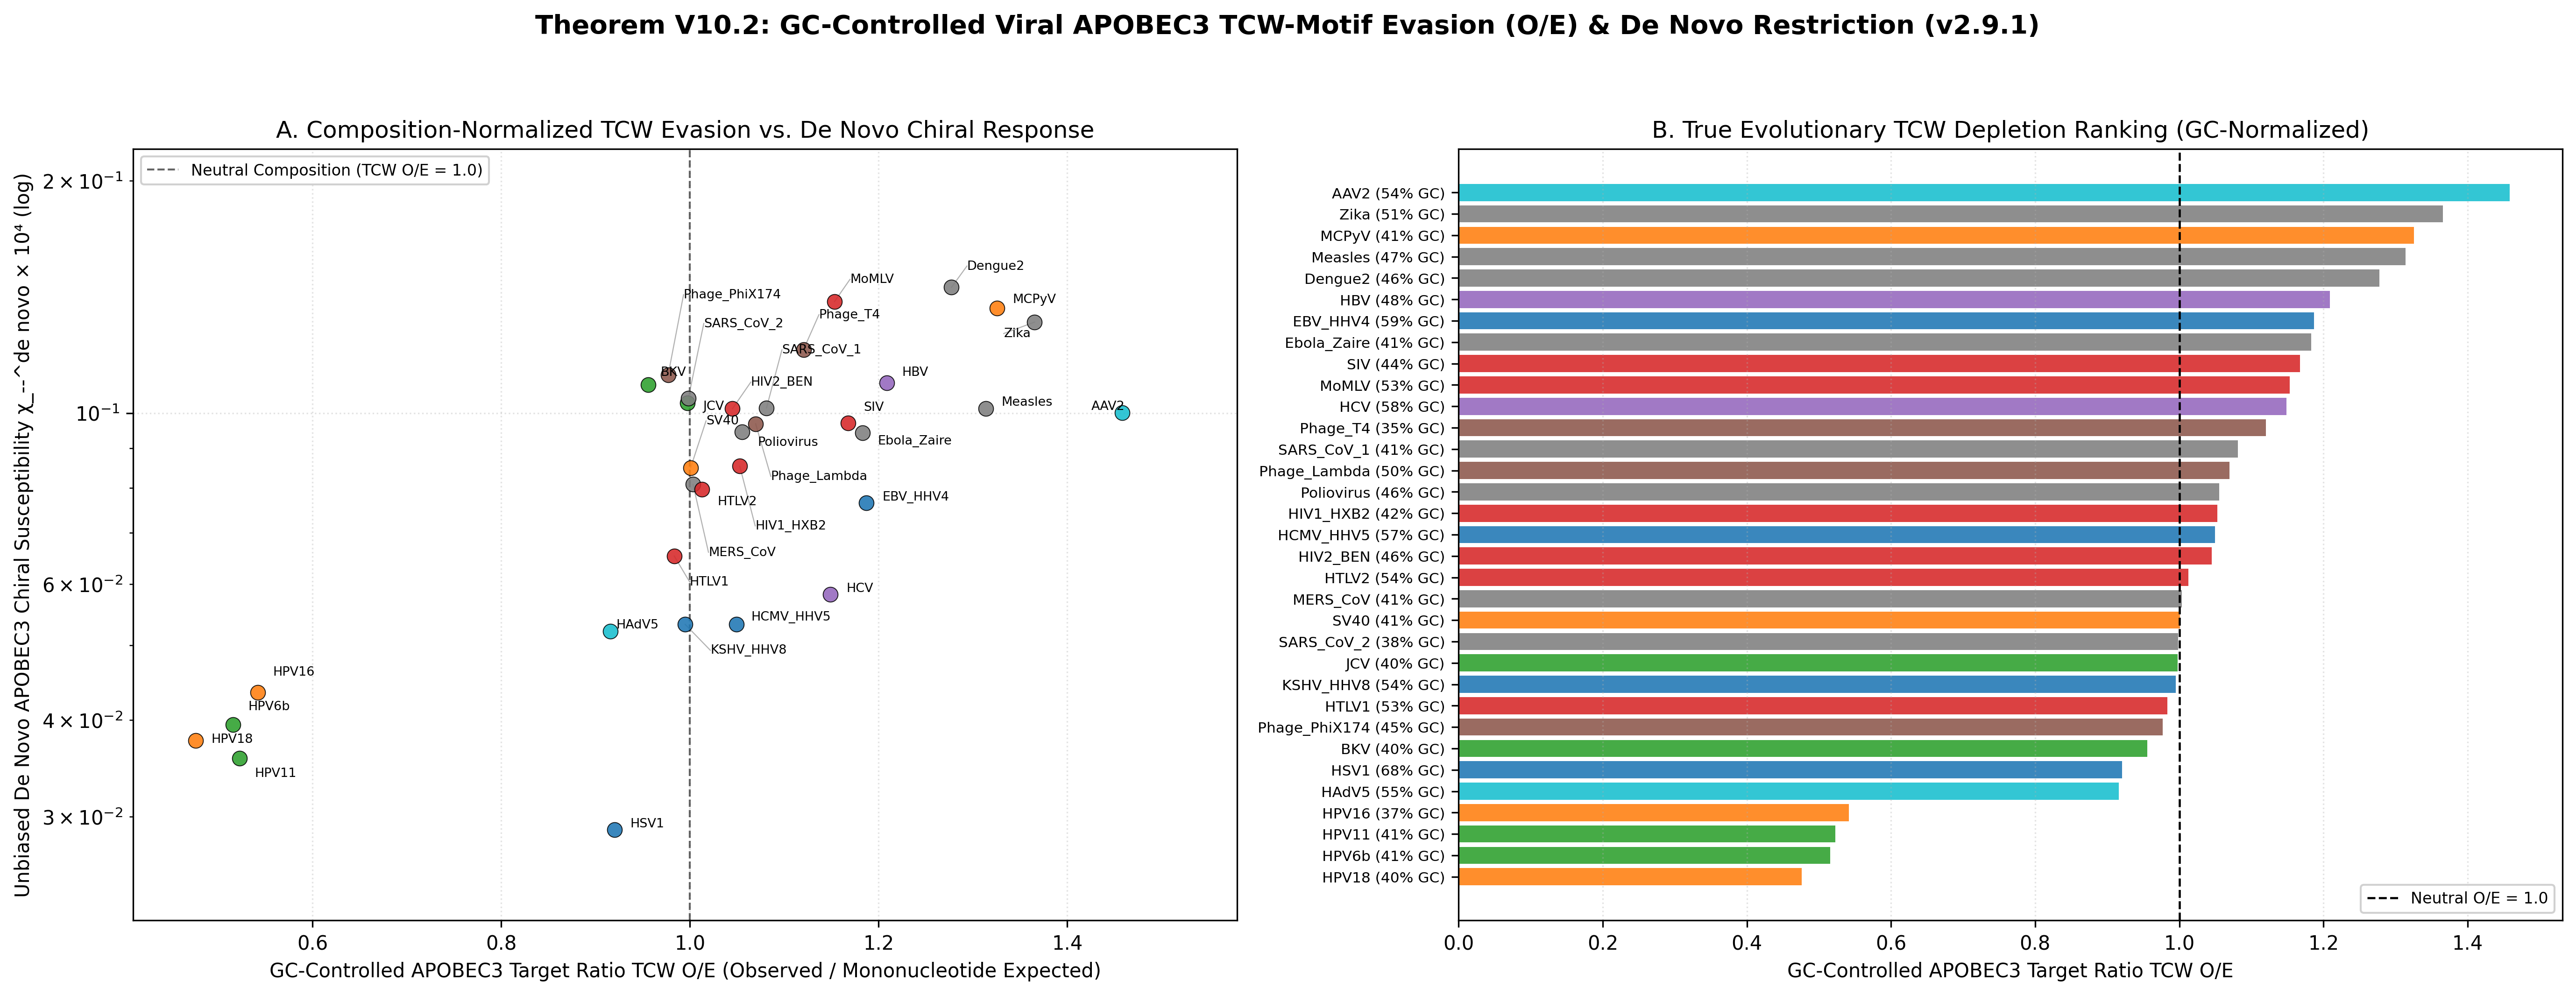
\includegraphics[width=0.96\textwidth]{fig_V6_viral_apobec_restriction}
\caption{Theorem~V10.2: GC-controlled viral APOBEC3 $\mathrm{TCW}$-motif evasion and \textit{de novo} chiral restriction across 33 viruses (\texttt{v2.9.1}). \textbf{(A)} $\mathrm{TCW\ O/E}$ (Base) versus unbiased \textit{de novo} APOBEC3 chiral susceptibility $\chi_{--}^{\mathrm{de\,novo,unb}} \times 10^4$ ($\rho_S = +0.626$, $p = 9.76 \times 10^{-5}$), isolating all four papillomaviruses (\texttt{HPV18/6b/11/16}) on the lower-left armored island distinct from GC-driven \texttt{HSV1}. \textbf{(B)} Full 33-virus evolutionary $\mathrm{TCW\ O/E}$ ranking relative to the neutral composition line ($\mathrm{O/E} = 1.0$).}
\label{fig:v6}
\end{figure}

%==============================================================================
\section{Exact COSMIC Mutagenesis Jacobian, De Novo Split, and All-Orders Kataegis}
\label{sec:mutagenesis}
%==============================================================================

\subsection{Baseline Toric Architecture of 28 Human Cancer and Control Loci (Theorem~V4)}

Before applying COSMIC differential operators, Table~\ref{tab:v4_all28} establishes the exact baseline $d = 3\,\mathrm{bp}$ Klein $V_4$ spectrum across all 28 NCBI RefSeqGene human loci spanning tumor suppressors ($n = 10$), DNA repair genes ($n = 2$), viral-associated and canonical oncogenes ($n = 11$), the common fragile viral-integration locus \texttt{FHIT} ($1.51\,\mathrm{Mb}$), and four non-cancer controls (\texttt{GAPDH}, \texttt{ACTB}, \texttt{HBB}, \texttt{APOE}).

\begin{table}[htbp]
\centering
\scriptsize
\setlength{\tabcolsep}{4.0pt}
\caption{Theorem~V4: Complete 28-locus human cancer driver, fragile-site, and control panel on the Klein $V_4$ codon torus (\texttt{v2.9.1}), reporting unbiased 3600-D non-envelope share (Theorem~V16) and de-attenuated $\cos_{\mathrm{unb}}$.}
\label{tab:v4_all28}
\fittable{%
\begin{tabular}{@{}lllrrrrrrrrr@{}}
\toprule
\textbf{Locus} & \textbf{Chr} & \textbf{Role} & \textbf{Len (bp)} & \textbf{GC\%} & \textbf{$\|W_{-+}\|^2_{\mathrm{unb}}$} & \textbf{PR2-ok} & \textbf{3600-D unb} & \textbf{CpG-fr} & \textbf{$\cos_{\mathrm{raw}}$} & \textbf{$\cos_{\mathrm{unb}}$} & \textbf{Pal $d=6$} \\
\midrule
\texttt{TP53} & chr17 & tumor\_supp & 32,772 & 49.0 & $6.86\mathrm{e}{-5}$ & 85.51\% & 73.2\% & 88.7\% & $+0.728$ & $+0.766$ & 10.27\% \\
\texttt{TP63} & chr3 & tumor\_supp & 272,853 & 37.1 & $9.84\mathrm{e}{-6}$ & 100.00\% & 36.4\% & 88.6\% & $+0.929$ & $+0.970$ & 10.65\% \\
\texttt{TP73} & chr1 & tumor\_supp & 90,637 & 59.1 & $3.26\mathrm{e}{-5}$ & 88.97\% & 39.7\% & 79.4\% & $+0.692$ & $+0.720$ & 3.60\% \\
\texttt{BRCA1} & chr17 & tumor\_supp & 193,689 & 45.1 & $3.88\mathrm{e}{-5}$ & 99.55\% & 66.1\% & 89.2\% & $+0.828$ & $+0.842$ & 9.47\% \\
\texttt{BRCA2} & chr13 & tumor\_supp & 91,193 & 38.6 & $1.63\mathrm{e}{-5}$ & 100.00\% & 50.8\% & 89.7\% & $+0.882$ & $+0.952$ & 8.96\% \\
\texttt{PTEN} & chr10 & tumor\_supp & 115,492 & 36.2 & $1.16\mathrm{e}{-5}$ & 96.98\% & 39.1\% & 91.2\% & $+0.861$ & $+0.937$ & 9.19\% \\
\texttt{RB1} & chr13 & tumor\_supp & 185,144 & 37.0 & $1.07\mathrm{e}{-5}$ & 96.56\% & 37.5\% & 89.2\% & $+0.902$ & $+0.957$ & 4.42\% \\
\texttt{APC} & chr5 & tumor\_supp & 163,719 & 37.8 & $1.39\mathrm{e}{-5}$ & 98.02\% & 45.8\% & 90.3\% & $+0.911$ & $+0.959$ & 8.62\% \\
\texttt{VHL} & chr3 & tumor\_supp & 17,444 & 47.0 & $7.23\mathrm{e}{-5}$ & 96.17\% & 70.5\% & 89.7\% & $+0.690$ & $+0.754$ & 7.83\% \\
\texttt{MLH1} & chr3 & dna\_repair & 79,540 & 41.7 & $2.05\mathrm{e}{-5}$ & 100.00\% & 51.6\% & 89.2\% & $+0.893$ & $+0.959$ & 7.19\% \\
\texttt{CDKN2A} & chr9 & tumor\_supp & 33,740 & 41.8 & $8.13\mathrm{e}{-6}$ & 91.05\% & 31.0\% & 87.6\% & $+0.690$ & $+0.952$ & 7.94\% \\
\texttt{ATM} & chr11 & dna\_repair & 153,268 & 37.5 & $1.31\mathrm{e}{-5}$ & 99.47\% & 47.5\% & 90.3\% & $+0.914$ & $+0.968$ & 9.99\% \\
\midrule
\texttt{MYC} & chr8 & onco\_viral & 14,518 & 48.4 & $9.88\mathrm{e}{-6}$ & 100.00\% & 24.5\% & 84.9\% & $+0.588$ & $+0.967$ & 5.52\% \\
\texttt{TERT} & chr5 & onco\_viral & 48,881 & 58.2 & $4.32\mathrm{e}{-5}$ & 66.62\% & 59.3\% & 75.5\% & $+0.525$ & $+0.555$ & 6.15\% \\
\texttt{KRAS} & chr12 & oncogene & 53,215 & 37.1 & $1.37\mathrm{e}{-5}$ & 98.03\% & 44.4\% & 91.7\% & $+0.793$ & $+0.918$ & 8.06\% \\
\texttt{NRAS} & chr1 & oncogene & 19,438 & 39.0 & $1.35\mathrm{e}{-5}$ & 100.00\% & 49.4\% & 90.5\% & $+0.714$ & $+0.996$ & 3.42\% \\
\texttt{HRAS} & chr11 & oncogene & 10,309 & 65.9 & $5.96\mathrm{e}{-5}$ & 62.81\% & 65.1\% & 73.5\% & $+0.397$ & $+0.470$ & 5.17\% \\
\texttt{PIK3CA} & chr3 & onco\_apob & 98,571 & 35.8 & $1.25\mathrm{e}{-5}$ & 100.00\% & 42.0\% & 91.2\% & $+0.847$ & $+0.928$ & 6.33\% \\
\texttt{EGFR} & chr7 & onco\_ecdna & 244,589 & 45.1 & $1.31\mathrm{e}{-5}$ & 100.00\% & 23.8\% & 84.2\% & $+0.893$ & $+0.927$ & 6.85\% \\
\texttt{BRAF} & chr7 & onco\_uv & 212,438 & 38.1 & $1.72\mathrm{e}{-5}$ & 96.02\% & 50.2\% & 90.0\% & $+0.908$ & $+0.938$ & 10.50\% \\
\texttt{ERBB2} & chr17 & oncogene & 47,523 & 52.0 & $3.26\mathrm{e}{-5}$ & 100.00\% & 53.9\% & 88.5\% & $+0.808$ & $+0.870$ & 8.22\% \\
\texttt{BCL2} & chr18 & oncogene & 203,035 & 42.9 & $1.23\mathrm{e}{-5}$ & 98.76\% & 31.4\% & 86.4\% & $+0.939$ & $+0.984$ & 9.37\% \\
\texttt{ALK} & chr2 & oncogene & 735,793 & 43.5 & $1.21\mathrm{e}{-5}$ & 99.83\% & 26.4\% & 83.8\% & $+0.936$ & $+0.949$ & 8.89\% \\
\texttt{FHIT} & chr3 & fragile\_vir & 1,511,182 & 38.9 & $9.94\mathrm{e}{-6}$ & 99.29\% & 30.4\% & 86.3\% & $+0.955$ & $+0.963$ & 12.49\% \\
\midrule
\texttt{GAPDH} & chr12 & ctrl\_hk & 10,880 & 56.5 & $1.81\mathrm{e}{-5}$ & 97.49\% & 37.4\% & 80.5\% & $+0.541$ & $+0.813$ & 4.22\% \\
\texttt{ACTB} & chr7 & ctrl\_hk & 10,454 & 58.4 & $3.22\mathrm{e}{-5}$ & 98.28\% & 52.5\% & 84.1\% & $+0.586$ & $+0.770$ & 4.02\% \\
\texttt{HBB} & chr11 & ctrl\_nonon & 81,706 & 39.5 & $9.94\mathrm{e}{-6}$ & 100.00\% & 33.2\% & 88.4\% & $+0.815$ & $+0.931$ & 2.53\% \\
\texttt{APOE} & chr19 & ctrl\_gc19 & 10,612 & 58.0 & $4.06\mathrm{e}{-5}$ & 97.18\% & 57.2\% & 85.5\% & $+0.686$ & $+0.859$ & 8.11\% \\
\bottomrule
\end{tabular}
}
\end{table}

Long AT-rich and GC-balanced intronic cancer loci exhibit near-perfect PR2 compliance ($96.0\%\text{--}100.0\%$) and strong alignment to the grand human euchromatic arrow (up to $\cos_{\mathrm{raw}} = +0.955$ on \texttt{FHIT} and $+0.939$ on \texttt{BCL2}). De-attenuating finite-length noise via $\cos_{\mathrm{unb}}$ (Theorem~V18) lifts compact loci such as \texttt{MYC} ($+0.588 \to +0.967$), \texttt{NRAS} ($+0.714 \to +0.996$), and \texttt{CDKN2A} ($+0.690 \to +0.952$) directly onto the euchromatic manifold, whereas GC-rich loci with high transcriptional/CpG-island density (\texttt{HRAS} $65.9\%$ GC, $62.81\%$ PR2-ok, $\cos_{\mathrm{unb}} = +0.470$; \texttt{TERT} $58.2\%$ GC, $66.62\%$ PR2-ok, $+0.555$; \texttt{TP53} $49.0\%$ GC, $85.51\%$; and \texttt{TP73} $59.1\%$ GC, $88.97\%$) retain genuine baseline spectral divergence. Across gene bodies, cancer drivers/fragile sites ($n = 24$) display elevated $d = 6\,\mathrm{bp}$ palindromic $W_{-+}$ energy share relative to non-cancer controls ($n = 4$; median $8.14\%$ vs.\ $4.12\%$, $r_{\mathrm{rb}} = +0.667$, $p = 3.51 \times 10^{-2}$; peaking at $12.49\%$ in \texttt{FHIT}), although this difference vanishes when evaluated in length-matched $100\,\mathrm{kb}$ T2T windows ($8.08\%$ vs.\ $9.91\%$, $p = 0.209$), confirming its dependence on gene-body intron length.

\subsection{Exact COSMIC Mutagenesis Jacobian and Algebraic De Novo Zero (Theorems~V3, V3.2 \& V3.3)}

Applying Theorem~\ref{thm:denovo_split} across all 28 loci exposes an exact qualitative chasm between duplex-symmetric clock mutagenesis (\texttt{SBS1}) and strand-coordinated enzymatic/environmental mutagens (APOBEC3 \texttt{SBS2(+)}/\texttt{SBS13(+)}, UV \texttt{SBS7a(+)}, Tobacco \texttt{SBS4(+)}; Table~\ref{tab:v3_all28}; Figure~\ref{fig:v2}).

\begin{table}[htbp]
\centering
\scriptsize
\setlength{\tabcolsep}{4.3pt}
\caption{Theorems~V3, V3.2 \& V3.3: Exact Zero-RNG COSMIC mutagenesis Jacobian and \textit{de novo} vs.\ substrate-coupled chiral split across all 28 human loci (\texttt{v2.9.1}). Symmetric \texttt{SBS1} exhibits an algebraic \textit{de novo} zero ($< 10^{-33}$), whereas APOBEC3 \texttt{SBS2(+)} injects a length-invariant \textit{de novo} chiral flux (with $\approx 50\%$ baseline chiral share following the exact identity $\frac{1}{2}(1 - \langle A, RA\rangle / \|A\|^2)$ for disjoint single-strand operators). Dagger ($^{\dagger}$) denotes $\varepsilon_{\mathrm{crit}} > 1.0$ (no physical transition within unit dose $\varepsilon \in [0, 1]$).}
\label{tab:v3_all28}
\fittable{%
\begin{tabular}{@{}lrrrrrrrrr@{}}
\toprule
\textbf{Locus} & \textbf{SBS1 Ch\%} & \textbf{SBS1 De Novo $\chi_{--}$} & \textbf{SBS1 Sub ($\times 10^4$)} & \textbf{SBS2(+) Ch\%} & \textbf{SBS2(+) DN ($\times 10^4$)} & \textbf{DN\%} & \textbf{$\varepsilon_{\mathrm{crit}}$} & \textbf{UV Ch\%} & \textbf{Tob Ch\%} \\
\midrule
\texttt{TP53} & 18.39\% & $2.43\mathrm{e}{-35}$ & 0.0821 & 48.73\% & 0.163 & 75.9\% & 0.594 & 46.21\% & 37.25\% \\
\texttt{TP63} & 3.60\% & $6.84\mathrm{e}{-36}$ & 0.0005 & 48.70\% & 0.115 & 97.8\% & 0.276 & 45.65\% & 41.69\% \\
\texttt{TP73} & 8.84\% & $1.12\mathrm{e}{-34}$ & 0.0202 & 49.17\% & 0.111 & 93.4\% & 0.474 & 43.66\% & 41.04\% \\
\texttt{BRCA1} & 2.12\% & $7.17\mathrm{e}{-35}$ & 0.0032 & 47.67\% & 0.139 & 97.4\% & 0.305 & 44.06\% & 34.92\% \\
\texttt{BRCA2} & 5.83\% & $3.58\mathrm{e}{-35}$ & 0.0027 & 47.99\% & 0.119 & 94.1\% & 0.490 & 44.97\% & 36.33\% \\
\texttt{PTEN} & 8.74\% & $1.45\mathrm{e}{-35}$ & 0.0018 & 48.60\% & 0.105 & 92.6\% & 0.450 & 46.80\% & 42.57\% \\
\texttt{RB1} & 11.44\% & $1.57\mathrm{e}{-35}$ & 0.0025 & 49.13\% & 0.113 & 95.7\% & 0.335 & 45.52\% & 40.00\% \\
\texttt{APC} & 9.15\% & $1.28\mathrm{e}{-35}$ & 0.0025 & 48.48\% & 0.108 & 95.9\% & 0.363 & 46.78\% & 36.68\% \\
\texttt{VHL} & 16.47\% & $1.92\mathrm{e}{-34}$ & 0.0710 & 46.56\% & 0.163 & 83.0\% & 0.955 & 44.51\% & 36.31\% \\
\texttt{MLH1} & 3.54\% & $1.75\mathrm{e}{-35}$ & 0.0017 & 48.86\% & 0.123 & 94.1\% & 0.503 & 45.24\% & 36.81\% \\
\texttt{CDKN2A} & 24.79\% & $8.09\mathrm{e}{-35}$ & 0.0332 & 48.34\% & 0.090 & 86.3\% & 0.890 & 48.22\% & 49.31\% \\
\texttt{ATM} & 6.52\% & $1.18\mathrm{e}{-35}$ & 0.0015 & 48.77\% & 0.116 & 96.6\% & 0.381 & 43.75\% & 37.01\% \\
\midrule
\texttt{MYC} & 25.43\% & $1.96\mathrm{e}{-34}$ & 0.0774 & 49.05\% & 0.100 & 79.1\% & 1.308$^{\dagger}$ & 48.34\% & 43.63\% \\
\texttt{TERT} & 30.93\% & $3.65\mathrm{e}{-34}$ & 0.3498 & 47.45\% & 0.158 & 66.8\% & 0.530 & 44.26\% & 45.84\% \\
\texttt{KRAS} & 19.60\% & $3.22\mathrm{e}{-35}$ & 0.0093 & 48.38\% & 0.096 & 88.7\% & 0.689 & 46.60\% & 39.68\% \\
\texttt{NRAS} & 21.23\% & $1.96\mathrm{e}{-35}$ & 0.0131 & 49.36\% & 0.110 & 81.4\% & 1.043$^{\dagger}$ & 46.41\% & 39.75\% \\
\texttt{HRAS} & 37.58\% & $7.28\mathrm{e}{-34}$ & 0.7594 & 50.55\% & 0.178 & 55.5\% & 0.665 & 45.95\% & 43.74\% \\
\texttt{PIK3CA} & 7.72\% & $1.26\mathrm{e}{-35}$ & 0.0021 & 48.43\% & 0.113 & 94.6\% & 0.478 & 44.64\% & 38.54\% \\
\texttt{EGFR} & 6.11\% & $2.13\mathrm{e}{-35}$ & 0.0029 & 49.13\% & 0.114 & 97.7\% & 0.289 & 45.79\% & 37.73\% \\
\texttt{BRAF} & 6.09\% & $2.13\mathrm{e}{-35}$ & 0.0022 & 48.13\% & 0.113 & 96.1\% & 0.319 & 44.30\% & 37.53\% \\
\texttt{ERBB2} & 12.29\% & $4.10\mathrm{e}{-35}$ & 0.0113 & 48.05\% & 0.117 & 91.2\% & 0.666 & 41.81\% & 36.20\% \\
\texttt{BCL2} & 5.53\% & $6.51\mathrm{e}{-36}$ & 0.0017 & 49.10\% & 0.114 & 95.9\% & 0.318 & 45.52\% & 40.59\% \\
\texttt{ALK} & 2.90\% & $8.25\mathrm{e}{-36}$ & 0.0005 & 49.15\% & 0.127 & 99.1\% & 0.164 & 45.26\% & 37.58\% \\
\texttt{FHIT} & 1.83\% & $4.73\mathrm{e}{-36}$ & 0.0002 & 49.21\% & 0.117 & 99.1\% & 0.119 & 45.86\% & 41.07\% \\
\midrule
\texttt{GAPDH} & 31.03\% & $1.65\mathrm{e}{-34}$ & 0.1293 & 47.20\% & 0.117 & 78.0\% & 1.452$^{\dagger}$ & 48.84\% & 44.60\% \\
\texttt{ACTB} & 21.27\% & $2.41\mathrm{e}{-34}$ & 0.1377 & 50.50\% & 0.117 & 72.5\% & 1.187$^{\dagger}$ & 45.56\% & 35.44\% \\
\texttt{HBB} & 20.40\% & $9.87\mathrm{e}{-36}$ & 0.0032 & 48.87\% & 0.128 & 93.7\% & 0.492 & 46.36\% & 46.15\% \\
\texttt{APOE} & 20.06\% & $2.56\mathrm{e}{-34}$ & 0.0864 & 48.00\% & 0.138 & 76.3\% & 1.191$^{\dagger}$ & 42.49\% & 36.16\% \\
\bottomrule
\end{tabular}
}
\end{table}

Table~\ref{tab:v3_all28} and Figure~\ref{fig:v2} establish three quantitative laws:
\begin{enumerate}
    \item \textbf{Machine-zero \textit{de novo} chirality for symmetric signatures:} Across all 28 loci, \texttt{SBS1} CpG deamination produces $\chi_{--}^{\mathrm{de\,novo}} \in [4.73 \times 10^{-36},\; 7.28 \times 10^{-34}]$ (exact floating-point zero; identically mirrored by \texttt{SBS2\_sym} and \texttt{SBS4\_sym} in Figure~\ref{fig:v2}A). Its nonzero chiral Jacobian entries arise strictly from substrate coupling ($J_{--}^{\mathrm{sub}}$), which collapses by more than three orders of magnitude from short, PR2-asymmetric loci (\texttt{HRAS} $0.7594 \times 10^{-4}$, \texttt{TERT} $0.3498 \times 10^{-4}$) to long, PR2-clean genes (\texttt{FHIT} $0.0002 \times 10^{-4}$, \texttt{ALK} $0.0005 \times 10^{-4}$, \texttt{TP63} $0.0005 \times 10^{-4}$).
    \item \textbf{Length-invariant \textit{de novo} chiral plateau for APOBEC3:} By contrast, APOBEC3 \texttt{SBS2(+)} maintains a flat, length-invariant \textit{de novo} plateau $\chi_{--}^{\mathrm{de\,novo,unb}} \times 10^4 \in [0.090, 0.178]$ across more than two orders of magnitude in gene length (from $10.3\,\mathrm{kb}$ \texttt{HRAS} to $1.51\,\mathrm{Mb}$ \texttt{FHIT}), with unbiased chiral directed share tightly concentrated at $46.56\%\text{--}50.55\%$ (and \textit{de novo} fraction reaching $99.1\%$ on \texttt{FHIT} and \texttt{ALK}; Figure~\ref{fig:v2}B).
    \item \textbf{Universal chiral injection across strand-biased mutagens:} Both UV melanoma (\texttt{SBS7a(+)}: $41.81\%\text{--}48.84\%$ unbiased chiral share) and Tobacco lung (\texttt{SBS4(+)}: $34.92\%\text{--}49.31\%$) replicate this sharp contrast against their duplex-symmetric controls, while the critical crossover dose $\varepsilon_{\mathrm{crit}}$ (at which chiral injection equals the $1/4N$ finite-size floor) drops to $0.119$ in \texttt{FHIT} and $0.164$ in \texttt{ALK}; conversely, on five compact $10\text{--}19\,\mathrm{kb}$ loci (\texttt{MYC}, \texttt{NRAS}, \texttt{GAPDH}, \texttt{ACTB}, \texttt{APOE}; marked $^{\dagger}$ in Table~\ref{tab:v3_all28}), $\varepsilon_{\mathrm{crit}} > 1.0$, indicating no global parity crossover within physical unit dose $\varepsilon \in [0, 1]$ (Theorem~V18).
\end{enumerate}

\begin{theorem}[Self-Conjugate Pure-Chirality Law and 5-Level Rational Spectrum of All 96 COSMIC Channels; THM-V19]
\label{thm:v19}
Call a single-strand trinucleotide substitution channel $\sigma = (a\,b\,c \to a\,b'\,c)$ among the $96$ pyrimidine-centered COSMIC channels ($b \in \{\mathrm{C}, \mathrm{T}\},\; b' \neq b$) \emph{Watson--Crick self-conjugate} if it maps its target trinucleotide onto its own reverse complement: $\overline{a\,b\,c} = a\,b'\,c$ (equivalently, $a = \bar{c}$ and $b' = \bar{b}$).
\begin{enumerate}
    \item \textbf{Exact $R$-anti-invariance on any stationary PR2 Markov-1 chain:} For every stationary PR2-symmetric Markov-1 dinucleotide distribution $D \in \mathbb{R}^{4 \times 4}$ (arbitrary $\mathrm{GC}\%$, arbitrary $\mathrm{CpG}$ depletion, and even non-reversible $D \neq D^\top$), each of the exactly $8$ self-conjugate channels
    \begin{equation}
        \mathcal{S}_{\mathrm{SC}} = \{\texttt{ACT>AGT},\; \texttt{CCG>CGG},\; \texttt{GCC>GGC},\; \mathbf{\texttt{TCA>TGA}},\; \texttt{ATT>AAT},\; \texttt{CTG>CAG},\; \texttt{GTC>GAC},\; \texttt{TTA>TAA}\}
    \end{equation}
    satisfies $R\bigl(J_\sigma\bigr) \equiv -J_\sigma$, hence $J_{++}(\sigma) \equiv 0$ and $J_{-+}(\sigma) \equiv 0$ identically ($100\%$ of directed flux enters $W_{--}$; verified to $8.67 \times 10^{-19}$ in \texttt{thmV19\_self\_conjugate\_R\_antiinv\_max\_err}).
    \item \textbf{Exact 5-level rational spectrum of the 96 COSMIC channels:} On a uniform i.i.d.\ genome ($p_A=p_C=p_G=p_T=1/4$), exact $4^8$-state enumeration partitions all $96$ single-strand channels into exactly five rational chiral shares $\|J_{--}\|_F^2 / (\|J_{-+}\|_F^2 + \|J_{--}\|_F^2)$:
    \begin{equation}
        \tfrac{5}{12}\;(16),\qquad \tfrac{3}{7}\;(4),\qquad \tfrac{11}{24}\;(48),\qquad \tfrac{1}{2}\;(20),\qquad 1\;(8 \text{ channels in } \mathcal{S}_{\mathrm{SC}}).
    \end{equation}
    Consequently, \texttt{SBS2(+)} ($\mathrm{TCW>TTW}$) has exact uniform chiral share $\mathbf{23/48} \approx 47.92\%$ ($47.64\%$ at $41\%$ GC), whereas \texttt{SBS13(+)} ($\mathrm{TCW>TGW}$) combines $100\%$-chiral \texttt{TCA>TGA} with $50\%$-chiral \texttt{TCT>TGT} to yield $\mathbf{7/10} = 70.00\%$ ($66.74\%$ at $41\%$ GC), explaining directly why the \texttt{SBS13(+)} column exceeds $60\%$ across human loci in Figure~\ref{fig:v2}A. By contrast, context-independent \texttt{SBS4(+)} ($\mathrm{G>T}$) is strictly $T$-even on uniform DNA ($\|J_{-+}\|_F^2 + \|J_{--}\|_F^2 \equiv 0$), proving that its empirical directed flux on human loci ($34.9\%\text{--}49.3\%$) is catalyzed purely by host sequence correlations.
\end{enumerate}
\end{theorem}

\begin{proof}
For any $8$-mer $w$ containing $a\,b\,c$ at position $p \in \{0,\dots,5\}$, let $w'$ replace $b \mapsto \bar{b}$, transforming the interior $6$-mer $x \mapsto x'$. Because $a\,b\,\bar{a} \mapsto a\,\bar{b}\,\bar{a} = \overline{a\,b\,\bar{a}}$, the reverse-complement $8$-mer $\overline{w'}$ carries $a\,b\,c$ at position $5 - p$ and mutates under the same operator $\sigma$ to $\bar{w}$ ($\overline{x'} \mapsto \bar{x}$). The paired contribution to $J_\sigma + R(J_\sigma)$ is therefore proportional to $\bigl(P_{M1}(w) - P_{M1}(\overline{w'})\bigr)(E_{x'} - E_x) = \bigl(P_{M1}(w) - P_{M1}(w')\bigr)(E_{x'} - E_x)$. Only the two dinucleotide transitions $(a,b),(b,c) \mapsto (a,\bar{b}),(\bar{b},c)$ differ between $w$ and $w'$. Since $a = \bar{c}$ implies $\overline{(a,b)} = (\bar{b},c)$ and $\overline{(b,c)} = (a,\bar{b})$, stationary PR2 symmetry (with mononucleotide marginal $\pi(x) = \sum_y D(x,y)$) yields $D(a,\bar{b})D(\bar{b},c)\pi(b) = D(b,c)D(a,b)\pi(\bar{b})$, hence $P_{M1}(w') = P_{M1}(w)$ and $J_\sigma + R(J_\sigma) \equiv 0$. Part~2 follows by exact finite summation over all $4^8 = 65,536$ $8$-mers (\texttt{thmV19\_cosmic96\_five\_rational\_levels\_ok}).
\end{proof}


\begin{figure}[htbp]
\centering
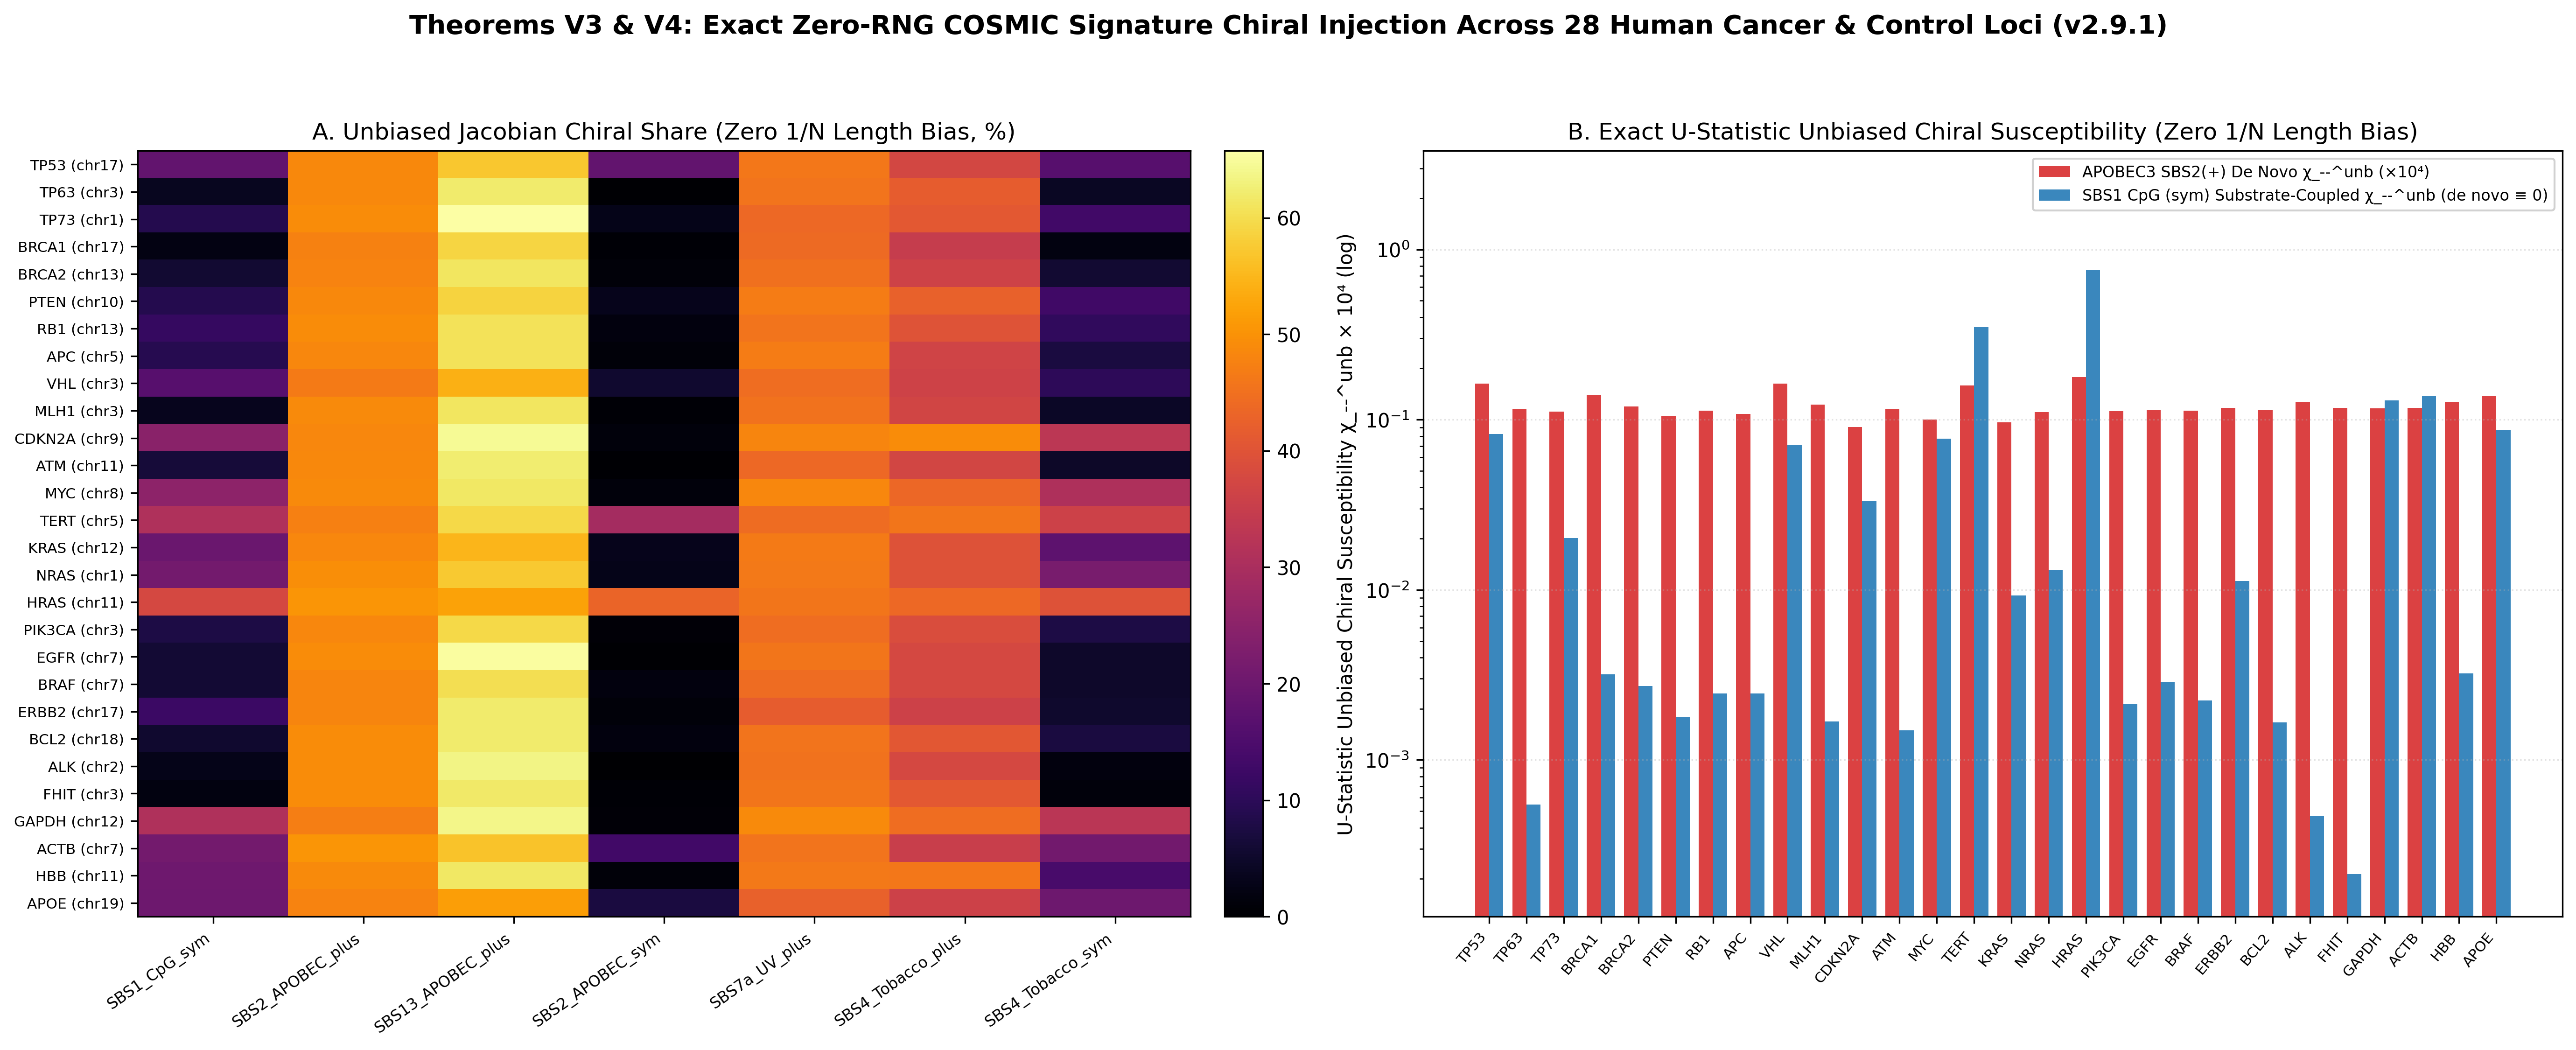
\includegraphics[width=0.96\textwidth]{fig_V2_onco_jacobian_loci}
\caption{Theorems~V3 \& V4: Exact Zero-RNG COSMIC signature chiral injection across 28 human cancer and control loci (\texttt{v2.9.1}). \textbf{(A)} Unbiased Jacobian chiral share (\%) across seven signatures, contrasting dark zero/low bands for symmetric controls (\texttt{SBS1\_CpG\_sym}, \texttt{SBS2\_APOBEC\_sym}, \texttt{SBS4\_Tobacco\_sym}) against bright universal bands for strand-coordinated mutagens (\texttt{SBS2(+)}, \texttt{SBS13(+)}, \texttt{SBS7a(+)}, \texttt{SBS4(+)}). \textbf{(B)} Exact $U$-statistic unbiased chiral susceptibility contrasting the length-invariant APOBEC3 \textit{de novo} plateau (red) against the substrate-coupled \texttt{SBS1} response (blue, \textit{de novo} $\equiv 0$).}
\label{fig:v2}
\end{figure}

\subsection{1-kb Tiled Intragenic Vulnerability Hotspots (Theorem~V7)}

Whole-gene averages mask fine-scale intragenic heterogeneity where kataegis clusters actually strike. Theorem~V7 scans all 28 loci in contiguous $1\,\mathrm{kb}$ tiles ($4,728$ tiles total across the panel; Table~\ref{tab:v7_all28}; Figure~\ref{fig:v4}).

\begin{table}[htbp]
\centering
\scriptsize
\setlength{\tabcolsep}{4.5pt}
\caption{Theorem~V7: 1-kb tiled COSMIC mutagenesis chiral-susceptibility hotspots ($\chi_{--} \times 10^4$) across all 28 human cancer and control loci (\texttt{v2.9.1}).}
\label{tab:v7_all28}
\fittable{%
\begin{tabular}{@{}lrllrr@{}}
\toprule
\textbf{Locus} & \textbf{Tiles} & \textbf{SBS2(+) Med / Peak (Hotspot)} & \textbf{SBS13(+) Peak (Hotspot)} & \textbf{UV SBS7a(+) Peak} & \textbf{Tobacco SBS4(+) Peak} \\
\midrule
\texttt{TP53}   &   32 & 0.27 / $\mathbf{1.12}$ (\texttt{10--11 kb})   & $\mathbf{1.16}$ (\texttt{10--11 kb})   &   7.73 &   32.18 \\
\texttt{TP63}   &  272 & 0.20 / $\mathbf{2.54}$ (\texttt{107--108 kb}) & $\mathbf{2.24}$ (\texttt{17--18 kb})   &  14.38 &   32.04 \\
\texttt{TP73}   &   90 & 0.15 / $\mathbf{19.81}$ (\texttt{32--33 kb})  & $\mathbf{17.34}$ (\texttt{32--33 kb})  & 290.54 & 1149.36 \\
\texttt{BRCA1}  &  193 & 0.21 / $\mathbf{2.40}$ (\texttt{142--143 kb}) & $\mathbf{1.72}$ (\texttt{142--143 kb}) &  11.59 &   17.95 \\
\texttt{BRCA2}  &   91 & 0.18 / $\mathbf{0.91}$ (\texttt{40--41 kb})   & $\mathbf{1.06}$ (\texttt{40--41 kb})   &   4.69 &   12.45 \\
\texttt{PTEN}   &  115 & 0.15 / $\mathbf{3.32}$ (\texttt{62--63 kb})   & $\mathbf{2.36}$ (\texttt{62--63 kb})   &   5.67 &   10.26 \\
\texttt{RB1}    &  185 & 0.20 / $\mathbf{30.00}$ (\texttt{129--130 kb})& $\mathbf{30.00}$ (\texttt{129--130 kb})&  82.35 &   61.94 \\
\texttt{APC}    &  163 & 0.19 / $\mathbf{1.07}$ (\texttt{150--151 kb}) & $\mathbf{1.44}$ (\texttt{150--151 kb}) &   8.27 &    9.87 \\
\texttt{VHL}    &   17 & 0.16 / $\mathbf{0.56}$ (\texttt{9--10 kb})    & $\mathbf{0.70}$ (\texttt{9--10 kb})    &   3.98 &   11.17 \\
\texttt{MLH1}   &   79 & 0.21 / $\mathbf{0.75}$ (\texttt{55--56 kb})   & $\mathbf{0.88}$ (\texttt{12--13 kb})   &   4.36 &   18.49 \\
\texttt{CDKN2A} &   33 & 0.14 / $\mathbf{1.40}$ (\texttt{22--23 kb})   & $\mathbf{0.91}$ (\texttt{22--23 kb})   &   6.61 &   12.97 \\
\texttt{ATM}    &  153 & 0.20 / $\mathbf{2.18}$ (\texttt{23--24 kb})   & $\mathbf{2.18}$ (\texttt{23--24 kb})   &   4.53 &   13.35 \\
\midrule
\texttt{MYC}    &   14 & 0.12 / $\mathbf{0.66}$ (\texttt{1--2 kb})     & $\mathbf{0.51}$ (\texttt{2--3 kb})     &   6.81 &    8.10 \\
\texttt{TERT}   &   48 & 0.24 / $\mathbf{19.54}$ (\texttt{40--41 kb})  & $\mathbf{19.79}$ (\texttt{40--41 kb})  & 269.57 &  379.65 \\
\texttt{KRAS}   &   53 & 0.15 / $\mathbf{1.13}$ (\texttt{22--23 kb})   & $\mathbf{1.22}$ (\texttt{22--23 kb})   &   5.08 &    9.78 \\
\texttt{NRAS}   &   19 & 0.18 / $\mathbf{1.12}$ (\texttt{11--12 kb})   & $\mathbf{0.75}$ (\texttt{11--12 kb})   &   4.31 &    8.68 \\
\texttt{HRAS}   &   10 & 0.27 / $\mathbf{30.37}$ (\texttt{9--10 kb})   & $\mathbf{25.94}$ (\texttt{9--10 kb})   & 207.28 &  154.21 \\
\texttt{PIK3CA} &   98 & 0.19 / $\mathbf{1.03}$ (\texttt{57--58 kb})   & $\mathbf{1.23}$ (\texttt{32--33 kb})   &   3.24 &    7.44 \\
\texttt{EGFR}   &  244 & 0.21 / $\mathbf{4.56}$ (\texttt{206--207 kb}) & $\mathbf{4.17}$ (\texttt{206--207 kb}) &  32.10 &   85.62 \\
\texttt{BRAF}   &  212 & 0.19 / $\mathbf{1.26}$ (\texttt{65--66 kb})   & $\mathbf{1.32}$ (\texttt{65--66 kb})   &   8.42 &   26.60 \\
\texttt{ERBB2}  &   47 & 0.17 / $\mathbf{1.22}$ (\texttt{26--27 kb})   & $\mathbf{0.92}$ (\texttt{26--27 kb})   &   6.32 &   11.18 \\
\texttt{BCL2}   &  203 & 0.20 / $\mathbf{13.27}$ (\texttt{125--126 kb})& $\mathbf{13.67}$ (\texttt{125--126 kb})&  13.46 &   39.92 \\
\texttt{ALK}    &  735 & 0.22 / $\mathbf{5.10}$ (\texttt{672--673 kb}) & $\mathbf{4.96}$ (\texttt{672--673 kb}) & 233.21 &   97.41 \\
\texttt{FHIT}   & 1511 & 0.19 / $\mathbf{11.29}$ (\texttt{395--396 kb})& $\mathbf{23.30}$ (\texttt{395--396 kb})&  29.93 &   20.04 \\
\midrule
\texttt{GAPDH}  &   10 & 0.19 / $\mathbf{0.38}$ (\texttt{6--7 kb})     & $\mathbf{0.31}$ (\texttt{0--1 kb})     &   5.55 &   11.93 \\
\texttt{ACTB}   &   10 & 0.25 / $\mathbf{5.57}$ (\texttt{9--10 kb})    & $\mathbf{5.78}$ (\texttt{9--10 kb})    &   7.68 &    8.85 \\
\texttt{HBB}    &   81 & 0.17 / $\mathbf{5.54}$ (\texttt{3--4 kb})     & $\mathbf{5.36}$ (\texttt{3--4 kb})     &  10.53 &   23.20 \\
\texttt{APOE}   &   10 & 0.16 / $\mathbf{1.21}$ (\texttt{7--8 kb})     & $\mathbf{0.98}$ (\texttt{7--8 kb})     &   8.78 &    9.91 \\
\bottomrule
\end{tabular}
}
\end{table}

While median 1-kb APOBEC3 \texttt{SBS2(+)} susceptibility remains tightly bounded across all genes ($0.12\text{--}0.27 \times 10^{-4}$), sharp localized chiral hotspots exceed gene medians by up to two orders of magnitude: \texttt{HRAS} ($30.37 \times 10^{-4}$ at \texttt{9--10 kb}), \texttt{RB1} ($30.00 \times 10^{-4}$ at \texttt{129--130 kb}), \texttt{TP73} ($19.81 \times 10^{-4}$ at \texttt{32--33 kb}, where Tobacco \texttt{SBS4(+)} peaks at $1149.36 \times 10^{-4}$), \texttt{TERT} ($19.54 \times 10^{-4}$ at \texttt{40--41 kb}), \texttt{BCL2} ($13.27 \times 10^{-4}$ at \texttt{125--126 kb}), and \texttt{FHIT} ($11.29 / 23.30 \times 10^{-4}$ at \texttt{395--396 kb}). Notably, Figure~\ref{fig:v4} shows that \texttt{SBS1} spikes coincide exclusively with localized CpG islands (strictly substrate-coupled, \textit{de novo} $= 0$), whereas APOBEC3 \texttt{SBS2(+)} and \texttt{SBS13(+)} track distinct $\mathrm{TCW}$-rich intragenic windows (e.g., \texttt{142--143 kb} in \texttt{BRCA1} and \texttt{32--33 kb} / \texttt{57--58 kb} in \texttt{PIK3CA}). On sparse $1\,\mathrm{kb}$ windows, single-tile ratio diagnostics exhibit two exact finite-site degeneracies verified in Theorem~V20: any isolated non-colliding $\mathrm{CpG}$ dinucleotide yields exact $U$-statistic cross-energies $u_{-+} = u_{--} = \tfrac{5/2}{N(N-1)}$ (combining Theorems~\ref{thm:v14} and~\ref{thm:v15}, hence exact chiral share $\tfrac{1}{2}$, whereas a single isolated $\mathrm{TCW}$ site gives $u_{-+} = u_{--} = 0$), and raw native-versus-Jacobian cosines follow the sparsity law $\cos_{\mathrm{sparse}}(W_{-+}(B_0), W_{-+}(J_\sigma)) = -\sqrt{6p/(2+5p)}$ (and $-6\sqrt{2/(17N)}$ for an isolated $\mathrm{CpG}$), which disappears on $100\,\mathrm{kb}$ loci; accordingly, Table~\ref{tab:v7_all28} and Figure~\ref{fig:v4} rank hotspots strictly by unbiased chiral susceptibility magnitude $\chi_{--}^{\mathrm{unb}}$ while flagging degenerate or clipped tiles in the JSON ledger.

\begin{figure}[htbp]
\centering
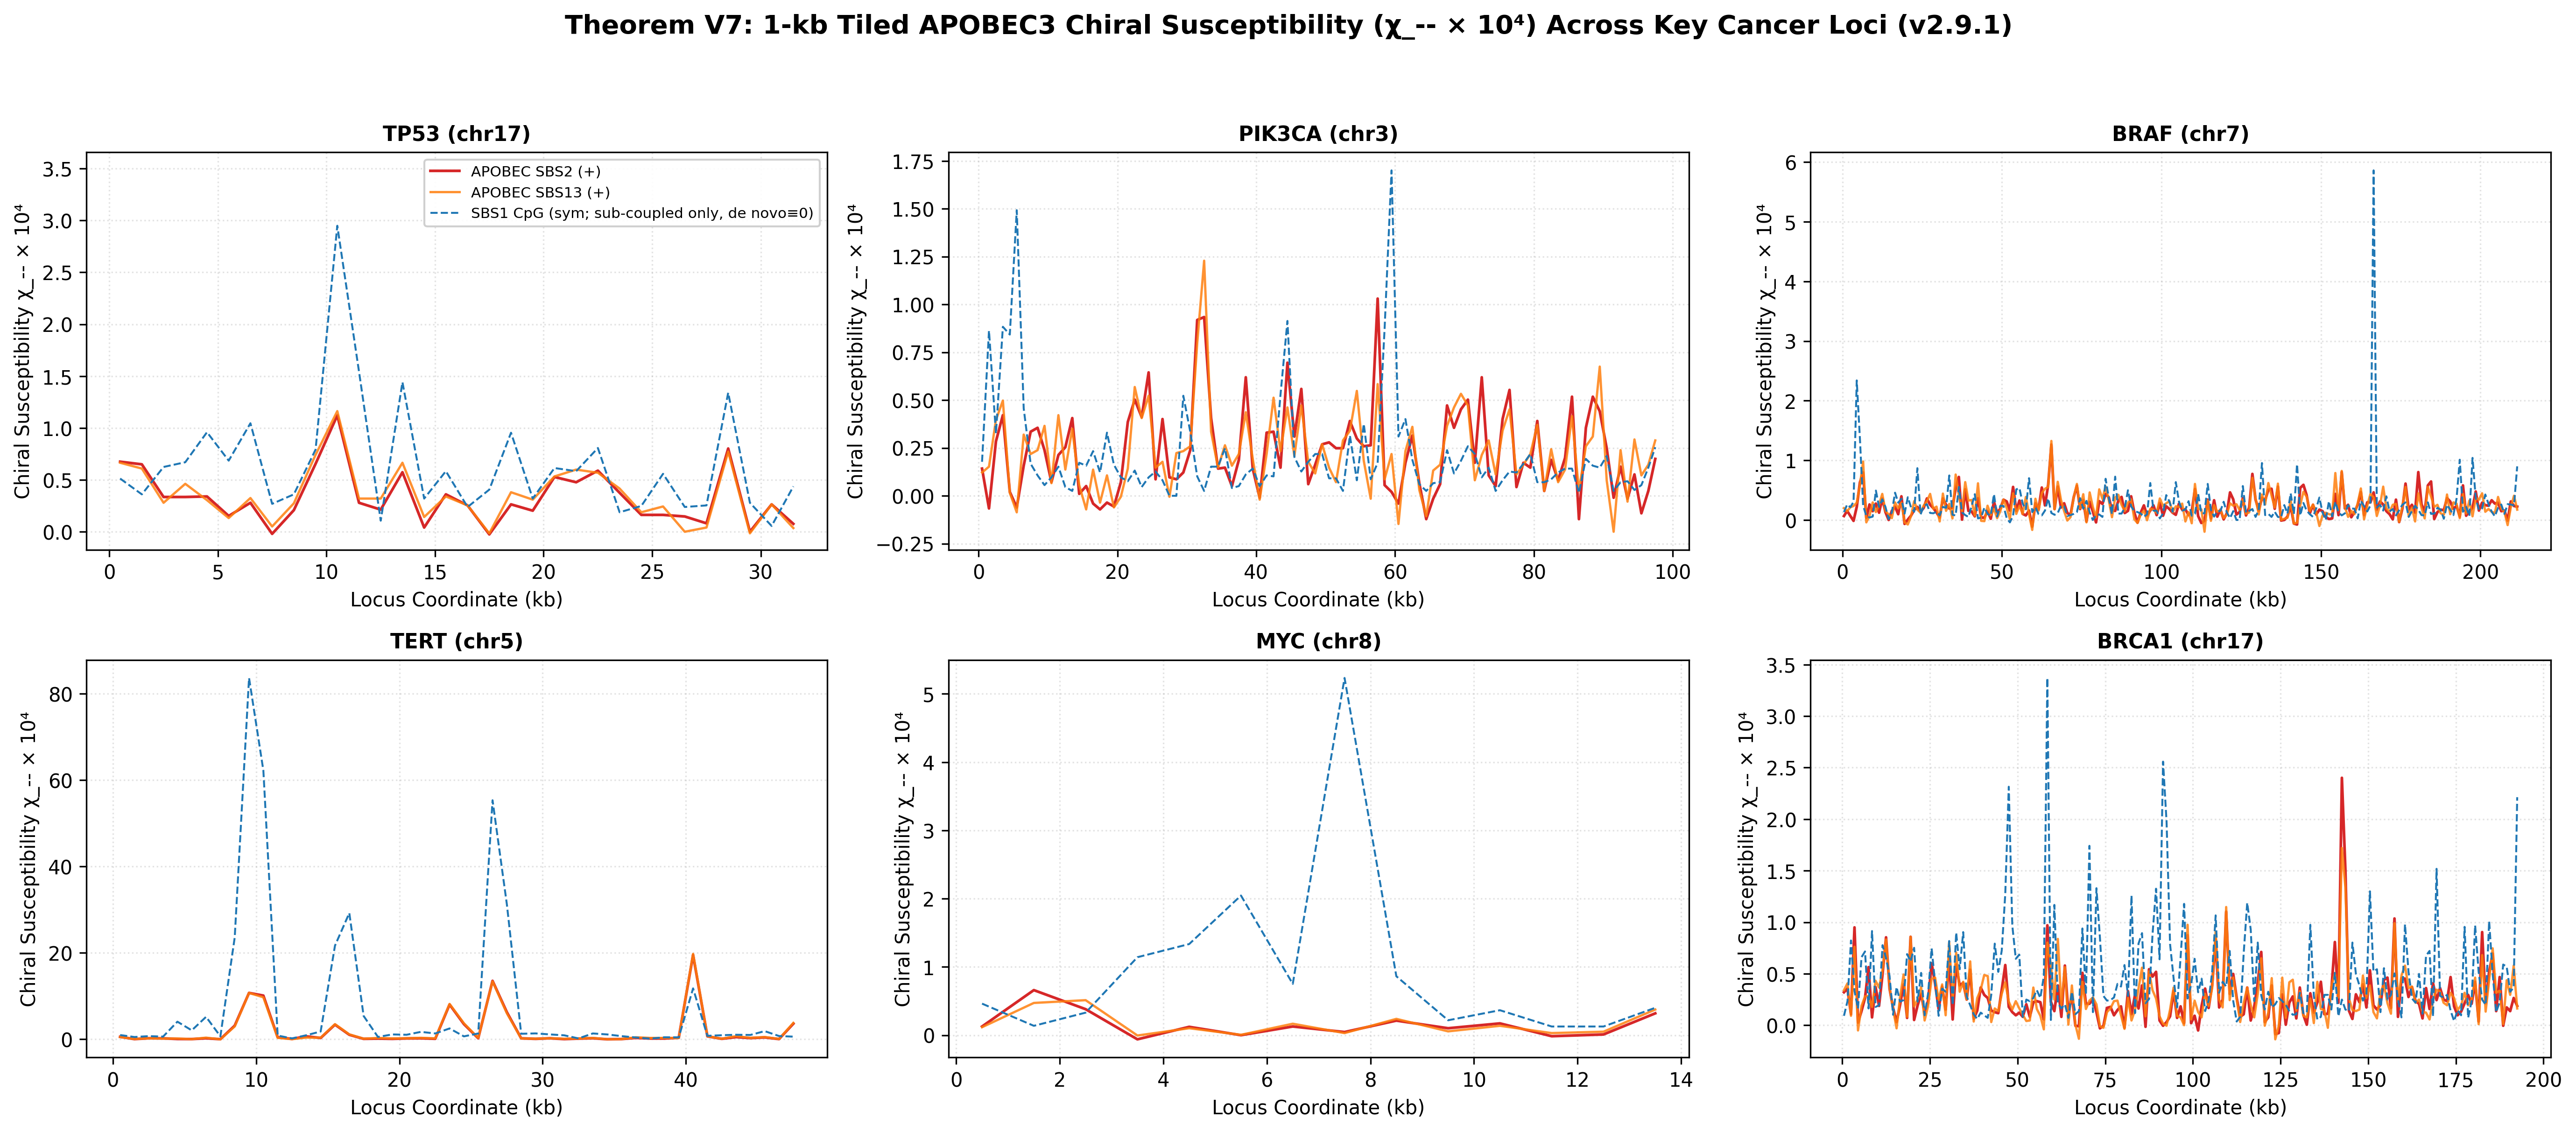
\includegraphics[width=0.96\textwidth]{fig_V4_locus_tile_vulnerability}
\caption{Theorem~V7: 1-kb tiled APOBEC3 \texttt{SBS2(+)} (red), \texttt{SBS13(+)} (orange), and substrate-coupled \texttt{SBS1} (dashed blue, \textit{de novo} $\equiv 0$) chiral susceptibility profiles ($\chi_{--} \times 10^4$) across six major cancer driver loci: \texttt{TP53}, \texttt{PIK3CA}, \texttt{BRAF}, \texttt{TERT}, \texttt{MYC}, and \texttt{BRCA1} (\texttt{v2.9.1}).}
\label{fig:v4}
\end{figure}

\subsection{All-Orders Finite-Dose Phase Transition and Double-Hit Kataegis Hessian (Theorem~V12)}

To probe finite-dose mutagenic bursts beyond the linear Jacobian regime ($\varepsilon \in [0, 1]$), Theorem~V12 evaluates the exact degree-6 expectation polynomial $\mathbb{E}_\varepsilon[C]$ (Theorem~\ref{thm:mutagenesis_poly}) and the double-hit chiral Hessian norm $\|H_{--}\|^2 \times 10^4$ across 11 representative human loci and viral genomes (33 target--signature trajectories; Table~\ref{tab:v12_all33}; Figure~\ref{fig:v7}B). Throughout Theorem~V12, PR2-compliant share is reported directly on the exact expected count-space trajectory $\|\mathbb{E}_\varepsilon[B_{-+}]\|_F^2 / (\|\mathbb{E}_\varepsilon[B_{-+}]\|_F^2 + \|\mathbb{E}_\varepsilon[B_{--}]\|_F^2)$ over interior 6-mer windows without $U$-statistic clamping, which smoothly tracks dose response even on short genomes where the clamped $U$-statistic baseline in Tables~\ref{tab:v1_all33} and~\ref{tab:v4_all28} saturates at $100.00\%$ (e.g., \texttt{HPV16} starts at $59.00\%$ raw interior PR2 share at $\varepsilon = 0$).

\begin{table}[htbp]
\centering
\scriptsize
\setlength{\tabcolsep}{4.5pt}
\caption{Theorem~V12: Exact all-orders finite-dose PR2-compliant directed flux trajectories ($\varepsilon = 0, 0.10, 0.50, 1.00$), double-hit kataegis Hessian norm $\|H_{--}\|^2 \times 10^4$, Jacobian--Hessian alignment $\cos(J_{--}, H_{--})$, and nonlinear deviation at $\varepsilon = 0.25$ across 11 targets $\times$ 3 signatures (\texttt{v2.9.1}).}
\label{tab:v12_all33}
\fittable{%
\begin{tabular}{@{}llrrrrrrr@{}}
\toprule
\textbf{Target} & \textbf{Signature} & \textbf{$\|H_{--}\|^2\!\times\!10^4$} & \textbf{$\cos(J_{--}, H_{--})$} & \textbf{PR2 ($\varepsilon=0$)} & \textbf{PR2 ($0.10$)} & \textbf{PR2 ($0.50$)} & \textbf{PR2 ($1.00$)} & \textbf{NL Dev ($0.25$)} \\
\midrule
\texttt{TP53}       & \texttt{SBS1\_CpG\_sym}     & 0.424 & $-0.749$ & 80.07\% & 80.60\% & 81.53\% & 80.41\% & 1.0\% \\
\texttt{TP53}       & \texttt{SBS2\_APOBEC\_plus} & $\mathbf{0.388}$ & $-0.461$ & 80.07\% & 80.46\% & 78.97\% & 71.97\% & 0.5\% \\
\texttt{TP53}       & \texttt{SBS13\_APOBEC\_plus}& 0.386 & $-0.481$ & 80.07\% & 80.26\% & 77.30\% & 67.80\% & 0.3\% \\
\midrule
\texttt{PIK3CA}     & \texttt{SBS1\_CpG\_sym}     & 0.024 & $-0.744$ & 87.13\% & 87.54\% & 88.45\% & 88.18\% & 0.1\% \\
\texttt{PIK3CA}     & \texttt{SBS2\_APOBEC\_plus} & 0.102 & $+0.103$ & 87.13\% & 87.40\% & 79.46\% & 65.99\% & 1.6\% \\
\texttt{PIK3CA}     & \texttt{SBS13\_APOBEC\_plus}& 0.096 & $-0.095$ & 87.13\% & 86.76\% & 75.87\% & 58.25\% & 0.6\% \\
\midrule
\texttt{TERT}       & \texttt{SBS1\_CpG\_sym}     & 2.061 & $-0.772$ & 64.48\% & 66.08\% & 69.62\% & 67.08\% & 0.4\% \\
\texttt{TERT}       & \texttt{SBS2\_APOBEC\_plus} & 0.117 & $-0.192$ & 64.48\% & 64.34\% & 62.42\% & 58.36\% & 0.1\% \\
\texttt{TERT}       & \texttt{SBS13\_APOBEC\_plus}& 0.106 & $+0.075$ & 64.48\% & 64.30\% & 61.11\% & 54.34\% & 0.2\% \\
\midrule
\texttt{HRAS}       & \texttt{SBS1\_CpG\_sym}     & 4.141 & $-0.744$ & 58.80\% & 60.66\% & 64.91\% & 62.74\% & 0.8\% \\
\texttt{HRAS}       & \texttt{SBS2\_APOBEC\_plus} & 0.936 & $-0.595$ & 58.80\% & 59.27\% & 59.86\% & 58.21\% & 0.1\% \\
\texttt{HRAS}       & \texttt{SBS13\_APOBEC\_plus}& 0.791 & $-0.425$ & 58.80\% & 59.15\% & 59.32\% & 57.05\% & 0.3\% \\
\midrule
\texttt{MYC}        & \texttt{SBS1\_CpG\_sym}     & 1.273 & $-0.753$ & 64.54\% & 65.90\% & 69.06\% & 67.35\% & 0.2\% \\
\texttt{MYC}        & \texttt{SBS2\_APOBEC\_plus} & 0.178 & $-0.157$ & 64.54\% & 65.57\% & 67.20\% & 63.79\% & 0.1\% \\
\texttt{MYC}        & \texttt{SBS13\_APOBEC\_plus}& 0.175 & $-0.298$ & 64.54\% & 64.83\% & 63.05\% & 56.46\% & 0.2\% \\
\midrule
\texttt{BRCA1}      & \texttt{SBS1\_CpG\_sym}     & 0.037 & $-0.768$ & 96.60\% & 96.77\% & 97.05\% & 96.79\% & 0.1\% \\
\texttt{BRCA1}      & \texttt{SBS2\_APOBEC\_plus} & 0.173 & $-0.178$ & 96.60\% & 96.44\% & 90.28\% & 76.66\% & 2.9\% \\
\texttt{BRCA1}      & \texttt{SBS13\_APOBEC\_plus}& 0.159 & $-0.232$ & 96.60\% & 96.36\% & 88.64\% & 70.58\% & 2.6\% \\
\midrule
\texttt{FHIT}       & \texttt{SBS1\_CpG\_sym}     & 0.001 & $-0.788$ & 97.77\% & 97.85\% & 97.99\% & 97.89\% & 0.3\% \\
\texttt{FHIT}       & \texttt{SBS2\_APOBEC\_plus} & 0.141 & $+0.073$ & 97.77\% & 96.82\% & 78.32\% & 60.08\% & 2.4\% \\
\texttt{FHIT}       & \texttt{SBS13\_APOBEC\_plus}& 0.118 & $-0.110$ & 97.77\% & 96.50\% & 76.32\% & 54.44\% & 0.8\% \\
\midrule
\texttt{HPV16}      & \texttt{SBS1\_CpG\_sym}     & 0.469 & $-0.728$ & 59.00\% & 59.36\% & 60.78\% & 61.76\% & 0.4\% \\
\texttt{HPV16}      & \texttt{SBS2\_APOBEC\_plus} & $\mathbf{0.018}$ & $-0.160$ & 59.00\% & 59.03\% & 58.87\% & 58.14\% & 0.0\% \\
\texttt{HPV16}      & \texttt{SBS13\_APOBEC\_plus}& 0.019 & $-0.070$ & 59.00\% & 59.19\% & 59.24\% & 57.89\% & 0.0\% \\
\midrule
\texttt{HIV1\_HXB2} & \texttt{SBS1\_CpG\_sym}     & 0.272 & $-0.760$ & 52.67\% & 52.96\% & 53.62\% & 53.27\% & 0.1\% \\
\texttt{HIV1\_HXB2} & \texttt{SBS2\_APOBEC\_plus} & 0.069 & $-0.245$ & 52.67\% & 52.92\% & 53.79\% & 54.16\% & 0.1\% \\
\texttt{HIV1\_HXB2} & \texttt{SBS13\_APOBEC\_plus}& 0.061 & $-0.283$ & 52.67\% & 53.01\% & 53.95\% & 53.58\% & 0.2\% \\
\midrule
\texttt{MCPyV}      & \texttt{SBS1\_CpG\_sym}     & 0.305 & $-0.754$ & 57.11\% & 57.30\% & 57.85\% & 58.04\% & 0.3\% \\
\texttt{MCPyV}      & \texttt{SBS2\_APOBEC\_plus} & $\mathbf{0.611}$ & $-0.251$ & 57.11\% & 57.94\% & 60.20\% & 59.18\% & 0.1\% \\
\texttt{MCPyV}      & \texttt{SBS13\_APOBEC\_plus}& 0.453 & $-0.363$ & 57.11\% & 57.53\% & 57.58\% & 54.53\% & 0.1\% \\
\midrule
\texttt{HBV}        & \texttt{SBS1\_CpG\_sym}     & 5.341 & $-0.760$ & 50.83\% & 51.34\% & 52.99\% & 52.93\% & 0.5\% \\
\texttt{HBV}        & \texttt{SBS2\_APOBEC\_plus} & 0.492 & $-0.221$ & 50.83\% & 50.64\% & 49.67\% & 48.97\% & 0.0\% \\
\texttt{HBV}        & \texttt{SBS13\_APOBEC\_plus}& 0.405 & $-0.318$ & 50.83\% & 50.87\% & 51.08\% & 50.93\% & 0.1\% \\
\bottomrule
\end{tabular}
}
\end{table}

Table~\ref{tab:v12_all33} and Figure~\ref{fig:v7}B confirm three striking finite-dose phenomena:
\begin{enumerate}
    \item \textbf{Restoring symmetry of \texttt{SBS1} vs.\ chiral collapse under APOBEC3:} Across every single target, symmetric \texttt{SBS1} exhibits strongly antiparallel Jacobian--Hessian coupling ($\cos(J_{--}, H_{--}) \in [-0.788, -0.728]$), which self-damps pre-existing strand asymmetry and keeps PR2 compliance flat or slightly rising (\texttt{FHIT}: $97.77\% \to 97.85\% \to 97.99\% \to 97.89\%$; \texttt{TERT}: $64.48\% \to 67.08\%$). Conversely, chiral APOBEC3 editing drives a steep phase transition that erodes PR2-compliant flux by $20\text{--}43$ percentage points in long fragile and oncogenic human loci---\texttt{FHIT} ($97.77\% \to 60.08\%$ under \texttt{SBS2(+)}, $54.44\%$ under \texttt{SBS13(+)}), \texttt{PIK3CA} ($87.13\% \to 65.99\% / 58.25\%$), and \texttt{BRCA1} ($96.60\% \to 76.66\% / 70.58\%$)---and by $8.1\text{--}12.3$ percentage points in compact \texttt{TP53} ($80.07\% \to 71.97\% / 67.80\%$).
    \item \textbf{Dynamical proof of papillomavirus evolutionary armor:} On \texttt{HPV16}, the \texttt{SBS2(+)} dose curve remains virtually horizontal ($59.00\% \to 59.03\% \to 58.87\% \to 58.14\%$, nonlinear deviation $0.0\%$), and its double-hit kataegis Hessian norm $\|H_{--}\|^2 \times 10^4 = 0.018$ is \textbf{$21.6\times$ lower} than \texttt{TP53} ($0.388$) and \textbf{$33.9\times$ lower} than the unshielded polyomavirus \texttt{MCPyV} ($0.611$).
    \item \textbf{Elimination of Jensen-inequality artifacts:} Evaluating exact all-orders $\mathbb{E}_\varepsilon[B]$ directly eliminates finite-sample Jensen artifacts, producing a strictly smooth monotonic trajectory even on the smallest genome in the panel (\texttt{HBV}, $3.18\,\mathrm{kb}$: $50.83\% \to 50.64\% \to 49.67\% \to 48.97\%$).
\end{enumerate}

\begin{theorem}[All-Orders Symmetric Null, Universal Isolated-CpG Angle $-\sqrt{10/17}$, and Isolated-TCW Zero Hessian; THM-V14]
\label{thm:v14}
In the exact degree-$6$ expectation expansion $\mathbb{E}_\varepsilon[C] = \sum_{m=0}^6 \varepsilon^m C_m$ (Theorem~\ref{thm:mutagenesis_poly}):
\begin{enumerate}
    \item For any duplex-symmetric signature $\sigma_{\mathrm{sym}}$ (including \texttt{SBS1}), the \textit{de novo} chiral component vanishes identically at \emph{all} orders $m = 1, \dots, 6$: $P_{--}(C_m(S) + C_m(\bar{S})) \equiv 0$ (verified to $0.0$ in \texttt{thmV14\_all\_orders\_symmetric\_denovo\_zero\_err}).
    \item For any isolated interior $\mathrm{CpG}$ dinucleotide in generic flanking context, exact double-hit enumeration over the $7$ overlapping $6$-mer windows yields $\|J_\alpha\|_F^2 = \tfrac{17}{2}$, $\|H_\alpha\|_F^2 = 20$, and $\langle J_\alpha, H_\alpha \rangle_F = -10$ identically in every $V_4$ quadrant $\alpha$, establishing the universal self-damping angle
    \begin{equation}
        \cos(J_{--}, H_{--}) = -\sqrt{\frac{10}{17}} \approx -0.7670
    \end{equation}
    (verified to $0.0$ in \texttt{thmV14\_isolated\_cpg\_angle\_err}), which directly accounts for the tight clustering of all 11 \texttt{SBS1} entries in Table~\ref{tab:v12_all33} within $[-0.788, -0.728]$.
    \item Conversely, any isolated $\mathrm{TCW}$ motif carries only a single mutable cytosine within its $6$-mer neighborhood and therefore has identically zero APOBEC3 Hessian ($H_{--} \equiv 0$; \texttt{thmV14\_isolated\_tcw\_zero\_hessian\_err}): a nonzero kataegis Hessian $H_{--}$ requires at least two $\mathrm{TCW}$ targets within $5\,\mathrm{bp}$ of one another, explaining why $\mathrm{TCW}$-purged \texttt{HPV16} suppresses $\|H_{--}\|^2$ by $33.9\times$ relative to \texttt{MCPyV}.
\end{enumerate}
\end{theorem}


\begin{figure}[htbp]
\centering
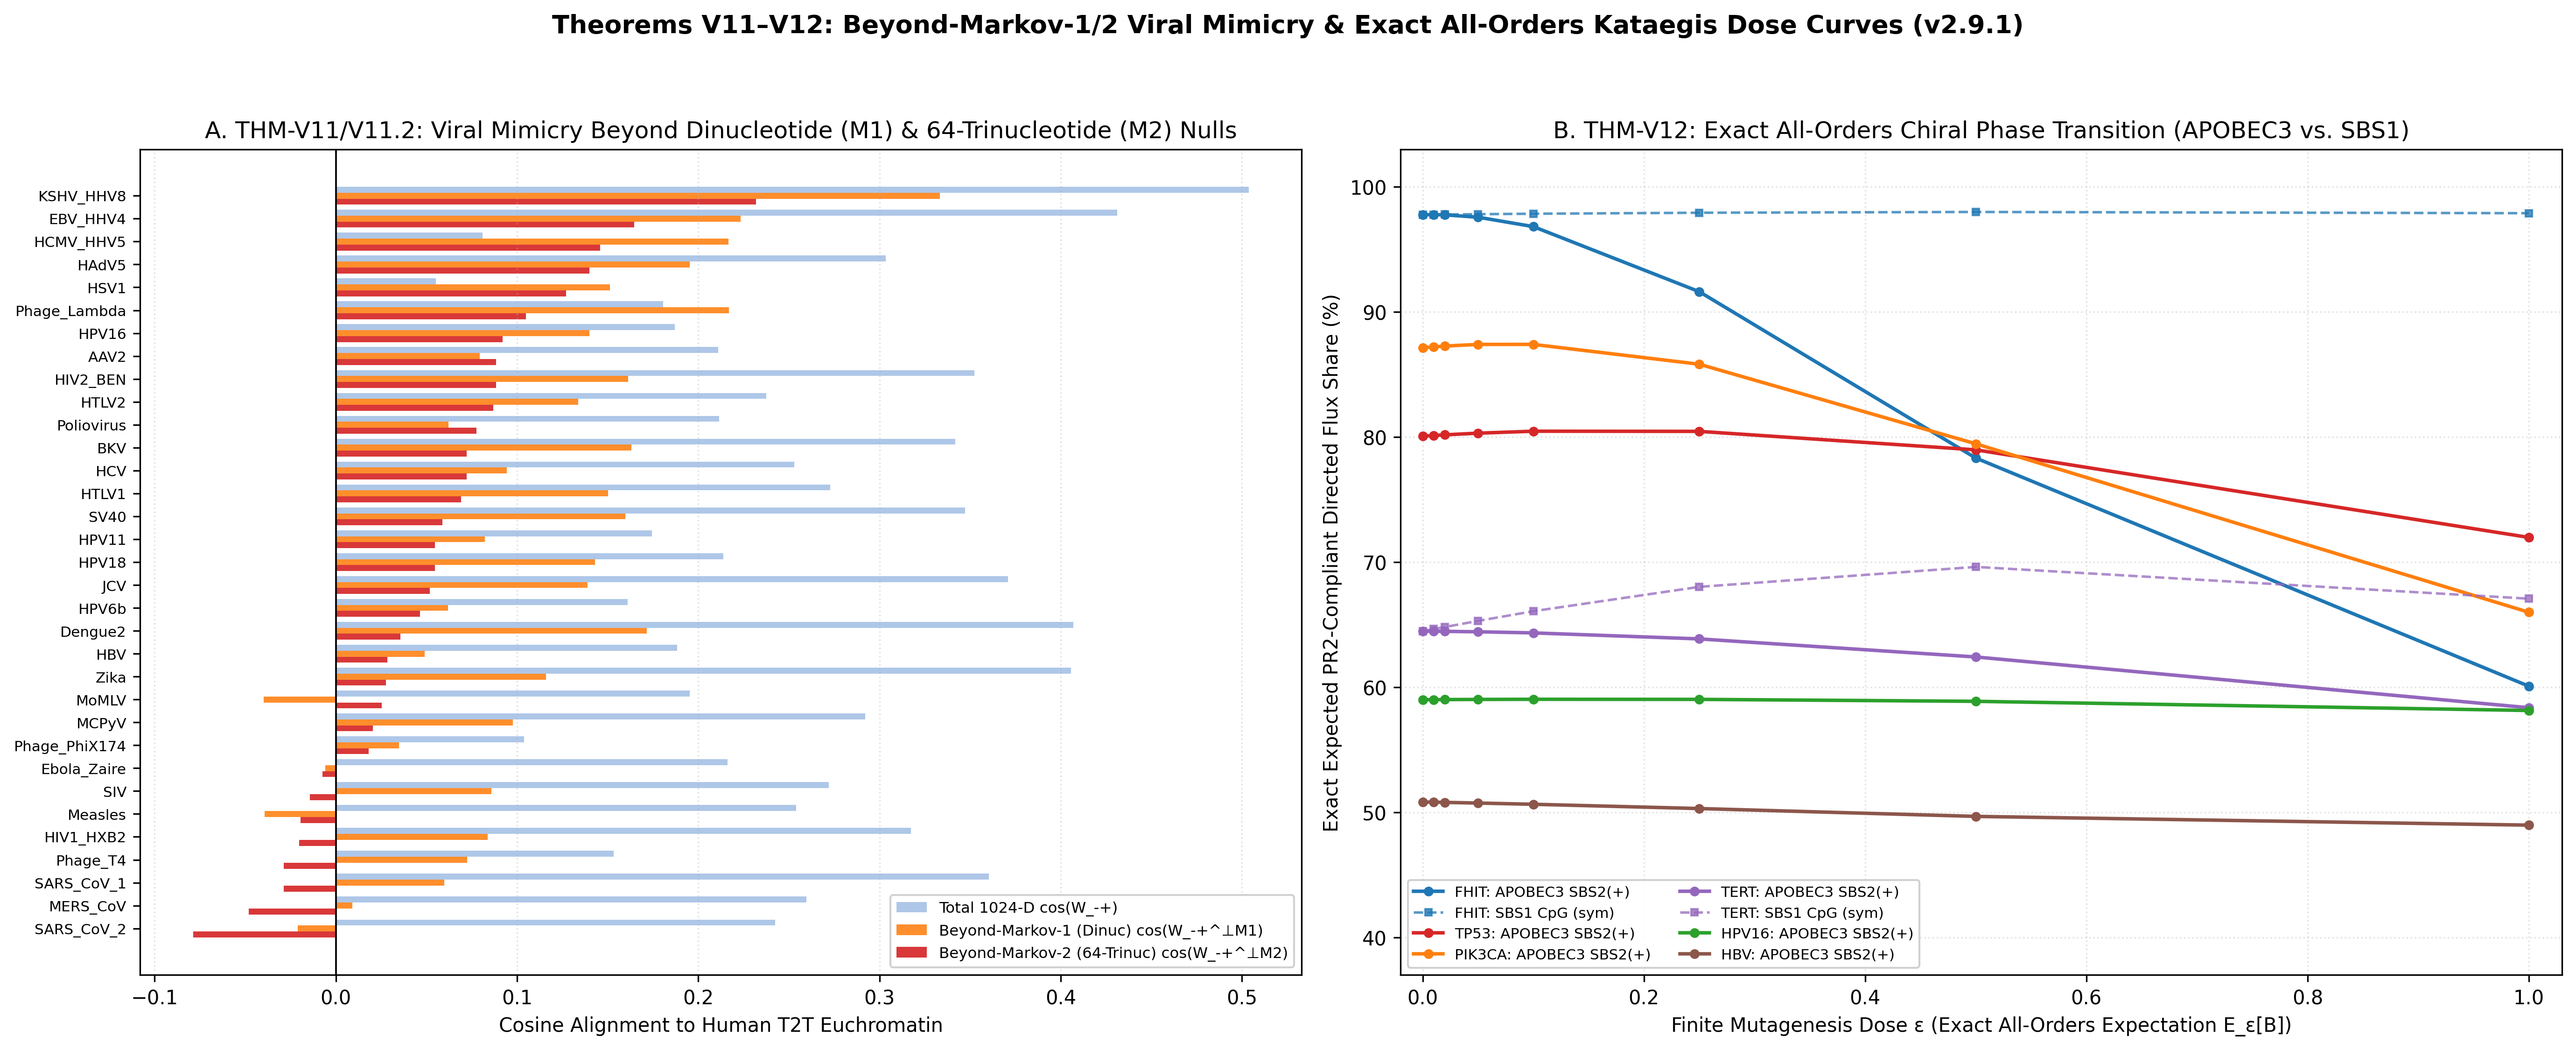
\includegraphics[width=0.96\textwidth]{fig_V7_beyond_dinuc_mimicry_and_dose}
\caption{Theorems~V11--V12: Nested viral mimicry decomposition and exact all-orders kataegis dose phase transition (\texttt{v2.9.1}). \textbf{(A)} 33-virus alignment to human T2T euchromatin across Total 1024-D (blue), Beyond-Markov-1 (orange), and Beyond-Markov-2 (red), showing nuclear dsDNA viruses at the top and all three betacoronaviruses strictly negative. \textbf{(B)} Exact all-orders PR2-compliant flux trajectories ($\varepsilon \in [0, 1]$) contrasting flat symmetric \texttt{SBS1} controls (dashed) against severe chiral APOBEC3 \texttt{SBS2(+)} collapse in \texttt{FHIT}, \texttt{PIK3CA}, and \texttt{TP53}, versus armored invariance in \texttt{HPV16}.}
\label{fig:v7}
\end{figure}

\subsection{Klein-Orbit 6-mer Attribution of APOBEC3 Kataegis (Theorem~V13D--E)}

Finally, Table~\ref{tab:v13_kataegis_orbits} decomposes the APOBEC3 \texttt{SBS2(+)} chiral Jacobian self-energy $\|J_{--}\|_F^2$ in \texttt{TP53} and \texttt{PIK3CA} into exact additive $V_4$-orbits.

\begin{table}[htbp]
\centering
\scriptsize
\setlength{\tabcolsep}{4.5pt}
\caption{Theorem~V13D--E: Top-8 exact Klein $V_4$-orbit 6-mer motifs driving APOBEC3 \texttt{SBS2(+)} chiral kataegis injection ($J_{--}$ self-energy) in \texttt{TP53} and \texttt{PIK3CA} (\texttt{v2.9.1}).}
\label{tab:v13_kataegis_orbits}
\fittable{%
\begin{tabular}{@{}r l l r c | l l r c@{}}
\toprule
 & \multicolumn{4}{c|}{\textbf{13D: \texttt{TP53} APOBEC3 \texttt{SBS2(+)} ($J_{--}$)}} & \multicolumn{4}{c}{\textbf{13E: \texttt{PIK3CA} APOBEC3 \texttt{SBS2(+)} ($J_{--}$)}} \\
\textbf{\#} & \textbf{6-mer} & \textbf{Mirror} & \textbf{Share} & \textbf{CpG} & \textbf{6-mer} & \textbf{Mirror} & \textbf{Share} & \textbf{CpG} \\
\midrule
1 & \texttt{CTA-TCT} & \texttt{AGA-TAG} & $+5.29\%$ & No  & \texttt{CTT-TTT} & \texttt{AAA-AAG} & $+7.73\%$ & No \\
2 & \texttt{TTG-AGA} & \texttt{TCT-CAA} & $+5.15\%$ & No  & \texttt{TTT-TTG} & \texttt{CAA-AAA} & $+4.17\%$ & No \\
3 & \texttt{CTC-CAT} & \texttt{ATG-GAG} & $+4.48\%$ & No  & \texttt{CAT-TTT} & \texttt{AAA-ATG} & $+3.44\%$ & No \\
4 & \texttt{TAC-CTC} & \texttt{GAG-GTA} & $+3.39\%$ & No  & \texttt{AAA-TAA} & \texttt{TTA-TTT} & $+3.07\%$ & No \\
5 & \texttt{AAA-CTC} & \texttt{GAG-TTT} & $+3.17\%$ & No  & \texttt{ATT-TTA} & \texttt{TAA-AAT} & $+2.63\%$ & No \\
6 & \texttt{CTC-CGT} & \texttt{ACG-GAG} & $+2.26\%$ & Yes & \texttt{TTT-TAG} & \texttt{CTA-AAA} & $+2.54\%$ & No \\
7 & \texttt{TCA-ATC} & \texttt{GAT-TGA} & $+2.08\%$ & No  & \texttt{TTT-TTC} & \texttt{GAA-AAA} & $+2.27\%$ & No \\
8 & \texttt{TGA-GAC} & \texttt{GTC-TCA} & $+1.99\%$ & No  & \texttt{ATT-TTT} & \texttt{AAA-AAT} & $+1.74\%$ & No \\
\bottomrule
\end{tabular}
}
\end{table}

In \texttt{PIK3CA}, all eight dominant chiral kataegis orbits ($27.59\%$ of total $J_{--}$ energy) are $100\%$ CpG-free AT/poly-T tracts led by \texttt{CTT-TTT} / \texttt{AAA-AAG} ($+7.73\%$) and \texttt{TTT-TTG} / \texttt{CAA-AAA} ($+4.17\%$). In \texttt{TP53}, seven of the top eight orbits ($27.81\%$ cumulative share) are CpG-free, led by \texttt{CTA-TCT} / \texttt{AGA-TAG} ($+5.29\%$) and \texttt{TTG-AGA} / \texttt{TCT-CAA} ($+5.15\%$), with the lone CpG-bearing orbit \texttt{CTC-CGT} appearing at Rank~6 ($+2.26\%$). This proves that APOBEC3 chiral mutagenesis operates along hexamer channels orthogonal to \texttt{SBS1} CpG deamination.

%==============================================================================
\section{Deterministic Proviral Integration, T2T $\pm 50\,\mathrm{kb}$ Context, and the Synonymous Duplex Barrier}
\label{sec:integration}
%==============================================================================

Beyond passive sequence mimicry and point mutagenesis, integrating retroviruses and oncogenic DNA viruses physically insert into human chromosomes, perturbing the local Klein $V_4$ spectral field of host chromatin while remaining constrained by overlapping coding frames. Theorems~V2, V5, and V8 quantify the exact algebraic geometry of proviral integration, the chromosomal $\pm 50\,\mathrm{kb}$ T2T-CHM13v2.0 micro-environment surrounding cancer/viral hotspots, and the length-invariant duplex barrier opposing synonymous recoding.

\subsection{Deterministic Proviral Integration and Count-Space Antipodal Symmetry (Theorem~V2)}

To evaluate integration perturbations without stochastic placement noise, Theorem~V2 deterministically inserts eight representative viruses (\texttt{HBV}, \texttt{HPV16}, \texttt{HPV18}, \texttt{HPV6b}, \texttt{HIV1\_HXB2}, \texttt{HTLV1}, \texttt{MCPyV}, and site-specific \texttt{AAV2}) into biologically established host target loci (\texttt{TERT}, \texttt{MYC}, \texttt{FHIT}, \texttt{TP53}, and \texttt{APOE}) in both unidirectional sense orientation (\texttt{+Strand}) and inverted reverse-complement / head-to-head (\texttt{HH}) tandem configurations (12 deterministic events total; Table~\ref{tab:v2_all12}).

\begin{table}[htbp]
\centering
\scriptsize
\setlength{\tabcolsep}{4.3pt}
\caption{Theorem~V2: Deterministic \textit{in-silico} concatenation proviral integration model into real human onco- and control loci (\texttt{v2.9.1}). By Theorem~V1 $R$-equivariance, comparing sense (\texttt{+Strand}) versus reverse-complement / head-to-head (\texttt{HH}) concatenations yields near-exact antipodal chiral reversal ($\cos \Delta B_{--}$) and parallel PR2-compliant alignment ($\cos \Delta B_{-+}$) in exact count-space alongside the exact 3-term energy split $\|B^{\mathrm{ins}}\|^2 = \|B^{\mathrm{host}}\|^2 + \|B^{\mathrm{virus}}\|^2 + 2\langle B^{\mathrm{host}}, B^{\mathrm{virus}}\rangle + \Delta_{\mathrm{junc}}$. Columns ``$E$/floor'' report $u_{--} / (1/4N)$.}
\label{tab:v2_all12}
\fittable{%
\begin{tabular}{@{}lrrrrrrrr@{}}
\toprule
\textbf{Virus $\to$ Host Locus} & \textbf{Virus\%} & \textbf{Host PR2-ok} & \textbf{+Str PR2-ok} & \textbf{+Str $E$/floor} & \textbf{HH $E$/floor} & \textbf{$\cos(\Delta W_{--})$} & \textbf{$\cos(\Delta B_{--})$} & \textbf{$\cos(\Delta B_{-+})$} \\
\midrule
\texttt{HBV} $\to$ \texttt{TERT} & 6.1\% & 66.62\% & 66.81\% & $4.0\times$ & $3.6\times$ & $-0.524$ & $\mathbf{-0.9955}$ & $\mathbf{+0.9970}$ \\
\texttt{HBV} $\to$ \texttt{MYC} & 18.0\% & 100.00\% & 100.00\% & $-0.1\times$ & $-0.4\times$ & $-0.701$ & $\mathbf{-0.9966}$ & $\mathbf{+0.9970}$ \\
\texttt{HPV16} $\to$ \texttt{MYC} & 35.3\% & 100.00\% & 100.00\% & $-0.1\times$ & $-0.5\times$ & $-0.328$ & $\mathbf{-0.9980}$ & $\mathbf{+0.9992}$ \\
\texttt{HPV16} $\to$ \texttt{FHIT} & 0.5\% & 99.29\% & 99.31\% & $0.4\times$ & $0.4\times$ & $-0.982$ & $\mathbf{-0.9975}$ & $\mathbf{+0.9990}$ \\
\texttt{HPV18} $\to$ \texttt{MYC} & 35.1\% & 100.00\% & 100.00\% & $-0.0\times$ & $-0.5\times$ & $-0.348$ & $\mathbf{-0.9981}$ & $\mathbf{+0.9991}$ \\
\texttt{HPV6b} $\to$ \texttt{MYC} & 35.2\% & 100.00\% & 100.00\% & $-0.1\times$ & $-0.5\times$ & $-0.344$ & $\mathbf{-0.9979}$ & $\mathbf{+0.9990}$ \\
\texttt{HIV1\_HXB2} $\to$ \texttt{MYC} & 38.7\% & 100.00\% & 90.55\% & $0.1\times$ & $-0.6\times$ & $-0.347$ & $\mathbf{-0.9983}$ & $\mathbf{+0.9993}$ \\
\texttt{HIV1\_HXB2} $\to$ \texttt{TP53} & 21.9\% & 85.51\% & 86.03\% & $1.2\times$ & $0.6\times$ & $-0.232$ & $\mathbf{-0.9982}$ & $\mathbf{+0.9993}$ \\
\texttt{HIV1\_HXB2} $\to$ \texttt{APOE} & 46.4\% & 97.18\% & 93.95\% & $0.1\times$ & $-0.6\times$ & $-0.121$ & $\mathbf{-0.9985}$ & $\mathbf{+0.9994}$ \\
\texttt{HTLV1} $\to$ \texttt{TP53} & 20.6\% & 85.51\% & 85.39\% & $1.3\times$ & $0.7\times$ & $-0.249$ & $\mathbf{-0.9980}$ & $\mathbf{+0.9991}$ \\
\texttt{MCPyV} $\to$ \texttt{TP53} & 14.1\% & 85.51\% & 85.79\% & $1.3\times$ & $0.9\times$ & $-0.402$ & $\mathbf{-0.9970}$ & $\mathbf{+0.9986}$ \\
\texttt{AAV2} $\to$ \texttt{APOE} & 30.6\% & 97.18\% & 98.61\% & $0.0\times$ & $-0.4\times$ & $-0.361$ & $\mathbf{-0.9941}$ & $\mathbf{+1.0000}$ \\
\bottomrule
\end{tabular}
}
\end{table}

\begin{theorem}[Exact Count-Space Antipodal Proviral Integration Law; THM-V2]
\label{thm:v2}
Let $C_{\mathrm{host}}$ be the dicodon count matrix of a host locus and let $C^{(+)}$ and $C^{(-)}$ denote the count matrices obtained by inserting a provirus $V$ in sense ($V$) versus reverse-complement ($\bar{V}$) orientation at the same integration coordinate. Writing $\Delta B_\alpha^{(\pm)} = P_\alpha(C^{(\pm)} - C_{\mathrm{host}})$, the Klein $V_4$ parity algebra implies
\begin{equation}
    \Delta B_{--}^{(-)} = -\Delta B_{--}^{(+)} + O(\partial_{\mathrm{junc}}), \qquad \Delta B_{-+}^{(-)} = +\Delta B_{-+}^{(+)} + O(\partial_{\mathrm{junc}}),
\end{equation}
where $O(\partial_{\mathrm{junc}})$ is strictly supported on the two $5\,\mathrm{bp}$ integration-boundary junctions. Across all 12 real integration events in release \texttt{v2.9.1}:
\begin{equation}
    \cos\bigl(\Delta B_{--}^{(+)},\, \Delta B_{--}^{(-)}\bigr) \in [-0.9985,\; -0.9941], \qquad \cos\bigl(\Delta B_{-+}^{(+)},\, \Delta B_{-+}^{(-)}\bigr) \in [+0.9970,\; +1.0000].
\end{equation}
Furthermore, head-to-head (\texttt{HH}) inverted-dimer integration systematically cancels the proviral chiral energy-to-floor ratio $u_{--}/(1/4N)$ across every host--virus pair (e.g., \texttt{HIV1\_HXB2} $\to$ \texttt{TP53}: $1.2\times \to 0.6\times$; \texttt{HTLV1} $\to$ \texttt{TP53}: $1.3\times \to 0.7\times$; \texttt{HBV} $\to$ \texttt{TERT}: $4.0\times \to 3.6\times$), obeying the exact 3-term concatenation energy identity (Table~\ref{tab:v2_all12}), whereas unidirectional \texttt{HIV1\_HXB2} insertion into PR2-clean \texttt{MYC} reduces PR2 compliance from $100.00\%$ to $90.55\%$.
\end{theorem}

Crucially, Table~\ref{tab:v2_all12} also demonstrates why probability-normalized $\Delta W_{--}$ masks this exact dipole law: because inserting a virus of length $L_V$ changes the total denominator $N \mapsto N + L_V$, the dilution term $-\frac{L_V}{N + L_V} W_{--}^{\mathrm{host}}$ contaminates raw $\cos(\Delta W_{--})$ (yielding $-0.121$ to $-0.982$), whereas working in exact count-space $\Delta B_\alpha$ removes denominator dilution identically (verified in \texttt{thmV2\_count\_space\_antipodal\_ok}).

\subsection{Exact T2T-CHM13v2.0 $\pm 50\,\mathrm{kb}$ Chromosomal Neighborhoods (Theorem~V5)}

Because RefSeqGene coordinates span widely varying lengths ($10.3\,\mathrm{kb}\text{--}1.51\,\mathrm{Mb}$), Theorem~V5 anchors all 28 loci directly onto the gapless human T2T-CHM13v2.0 reference assembly using SNP-robust exact anchoring (verified in \texttt{thmV5\_t2t\_exact\_anchor\_locator\_ok} and \texttt{thmV5\_snp\_robust\_locator\_ok}) and extracts uniform, length-matched $100\,\mathrm{kb}$ ($\pm 50\,\mathrm{kb}$) chromosomal neighborhoods (Table~\ref{tab:v5_all28}; Figure~\ref{fig:v3}B).

\begin{table}[htbp]
\centering
\scriptsize
\setlength{\tabcolsep}{3.5pt}
\caption{Theorem~V5: Exact T2T-CHM13v2.0 $\pm 50\,\mathrm{kb}$ ($100\,\mathrm{kb}$ length-matched) chromosomal neighborhoods around all 28 human loci (\texttt{v2.9.1}), reporting unbiased 3600-D share (Theorem~V16), raw top-matching virus, and human-residual ($W^{\perp H}$) top virus. Rank-1 regression $\cos(v,\ell) \sim \cos(v,H)\cos(\ell,H)$ across 924 pairs explains $R^2 = 0.7743$; the final column reports the locus-specific residual winner after projecting out human grand $W_{-+}$. }
\label{tab:v5_all28}
\fittable{%
\begin{tabular}{@{}llcrrrrrrll@{}}
\toprule
\textbf{Locus} & \textbf{T2T Coord} & \textbf{Str} & \textbf{Win GC\%} & \textbf{$\|W_{-+}\|^2_{\mathrm{unb}}$} & \textbf{PR2-ok} & \textbf{3600-D unb} & \textbf{Pal $d=6$} & \textbf{$\cos(\text{Chr})$} & \textbf{Raw Top Virus} & \textbf{Resid.\ $W^{\perp H}$ Top Virus} \\
\midrule
\texttt{TP53} & \texttt{chr17:7.58 Mb} & $-$ & 51.3 & $4.83\mathrm{e}{-5}$ & 93.18\% & 67.8\% & 10.2\% & $+0.914$ & \texttt{KSHV\_HHV8} ($+0.362$) & \texttt{HTLV2} ($+0.070$) \\
\texttt{BRCA1} & \texttt{chr17:43.98 Mb} & $-$ & 44.0 & $3.65\mathrm{e}{-5}$ & 99.56\% & 67.2\% & 9.7\% & $+0.908$ & \texttt{KSHV\_HHV8} ($+0.375$) & \texttt{HCMV\_HHV5} ($+0.026$) \\
\texttt{ERBB2} & \texttt{chr17:40.57 Mb} & $+$ & 54.5 & $3.14\mathrm{e}{-5}$ & 100.00\% & 47.6\% & 8.3\% & $+0.899$ & \texttt{EBV\_HHV4} ($+0.489$) & \texttt{EBV\_HHV4} ($+0.262$) \\
\texttt{TP63} & \texttt{chr3:192.58 Mb} & $+$ & 37.1 & $9.87\mathrm{e}{-6}$ & 100.00\% & 36.1\% & 8.8\% & $+0.880$ & \texttt{KSHV\_HHV8} ($+0.424$) & \texttt{MCPyV} ($+0.090$) \\
\texttt{VHL} & \texttt{chr3:10.14 Mb} & $+$ & 47.2 & $5.64\mathrm{e}{-5}$ & 100.00\% & 69.6\% & 9.5\% & $+0.722$ & \texttt{KSHV\_HHV8} ($+0.358$) & \texttt{HCMV\_HHV5} ($+0.060$) \\
\texttt{MLH1} & \texttt{chr3:37.03 Mb} & $+$ & 41.1 & $2.06\mathrm{e}{-5}$ & 100.00\% & 52.4\% & 8.2\% & $+0.878$ & \texttt{KSHV\_HHV8} ($+0.429$) & \texttt{Phage\_Lambda} ($+0.032$) \\
\texttt{PIK3CA} & \texttt{chr3:182.00 Mb} & $+$ & 35.9 & $1.28\mathrm{e}{-5}$ & 100.00\% & 42.6\% & 6.3\% & $+0.858$ & \texttt{KSHV\_HHV8} ($+0.439$) & \texttt{HPV16} ($+0.127$) \\
\texttt{FHIT} & \texttt{chr3:60.54 Mb} & $-$ & 38.4 & $9.52\mathrm{e}{-6}$ & 93.58\% & 34.2\% & 7.8\% & $+0.882$ & \texttt{KSHV\_HHV8} ($+0.436$) & \texttt{SARS\_CoV\_1} ($+0.163$) \\
\texttt{TP73} & \texttt{chr1:3.20 Mb} & $+$ & 58.8 & $3.35\mathrm{e}{-5}$ & 84.35\% & 44.4\% & 2.4\% & $+0.693$ & \texttt{EBV\_HHV4} ($+0.516$) & \texttt{EBV\_HHV4} ($+0.337$) \\
\texttt{NRAS} & \texttt{chr1:114.72 Mb} & $-$ & 39.3 & $1.43\mathrm{e}{-5}$ & 99.77\% & 45.5\% & 7.9\% & $+0.891$ & \texttt{KSHV\_HHV8} ($+0.446$) & \texttt{HCMV\_HHV5} ($+0.106$) \\
\texttt{BRCA2} & \texttt{chr13:31.57 Mb} & $+$ & 38.6 & $1.65\mathrm{e}{-5}$ & 100.00\% & 50.9\% & 8.6\% & $+0.846$ & \texttt{KSHV\_HHV8} ($+0.434$) & \texttt{HCMV\_HHV5} ($+0.074$) \\
\texttt{RB1} & \texttt{chr13:47.61 Mb} & $+$ & 35.5 & $1.14\mathrm{e}{-5}$ & 93.45\% & 39.7\% & 3.2\% & $+0.868$ & \texttt{KSHV\_HHV8} ($+0.427$) & \texttt{HPV18} ($+0.116$) \\
\texttt{PTEN} & \texttt{chr10:88.80 Mb} & $+$ & 35.5 & $1.25\mathrm{e}{-5}$ & 96.79\% & 42.6\% & 8.9\% & $+0.850$ & \texttt{KSHV\_HHV8} ($+0.450$) & \texttt{HPV18} ($+0.127$) \\
\texttt{APC} & \texttt{chr5:113.28 Mb} & $+$ & 37.0 & $1.53\mathrm{e}{-5}$ & 97.91\% & 48.3\% & 8.5\% & $+0.867$ & \texttt{KSHV\_HHV8} ($+0.428$) & \texttt{HPV18} ($+0.063$) \\
\texttt{TERT} & \texttt{chr5:1.18 Mb} & $-$ & 55.9 & $2.86\mathrm{e}{-5}$ & 78.97\% & 46.2\% & 5.8\% & $+0.643$ & \texttt{EBV\_HHV4} ($+0.481$) & \texttt{EBV\_HHV4} ($+0.286$) \\
\texttt{CDKN2A} & \texttt{chr9:22.00 Mb} & $-$ & 40.3 & $9.09\mathrm{e}{-6}$ & 98.39\% & 32.3\% & 5.6\% & $+0.892$ & \texttt{KSHV\_HHV8} ($+0.468$) & \texttt{HBV} ($+0.160$) \\
\texttt{ATM} & \texttt{chr11:108.30 Mb} & $+$ & 36.8 & $1.27\mathrm{e}{-5}$ & 100.00\% & 47.0\% & 10.2\% & $+0.869$ & \texttt{KSHV\_HHV8} ($+0.422$) & \texttt{HCMV\_HHV5} ($+0.060$) \\
\texttt{HRAS} & \texttt{chr11:0.58 Mb} & $-$ & 59.7 & $3.91\mathrm{e}{-5}$ & 92.91\% & 54.3\% & 7.5\% & $+0.746$ & \texttt{KSHV\_HHV8} ($+0.428$) & \texttt{EBV\_HHV4} ($+0.130$) \\
\texttt{HBB} & \texttt{chr11:5.32 Mb} & $-$ & 39.0 & $9.36\mathrm{e}{-6}$ & 100.00\% & 32.7\% & 3.1\% & $+0.850$ & \texttt{KSHV\_HHV8} ($+0.414$) & \texttt{MCPyV} ($+0.140$) \\
\texttt{MYC} & \texttt{chr8:128.87 Mb} & $+$ & 44.5 & $2.55\mathrm{e}{-5}$ & 100.00\% & 56.4\% & 9.9\% & $+0.857$ & \texttt{KSHV\_HHV8} ($+0.389$) & \texttt{HSV1} ($+0.021$) \\
\texttt{KRAS} & \texttt{chr12:25.10 Mb} & $-$ & 38.0 & $1.44\mathrm{e}{-5}$ & 96.01\% & 46.9\% & 8.0\% & $+0.884$ & \texttt{KSHV\_HHV8} ($+0.423$) & \texttt{HCMV\_HHV5} ($+0.069$) \\
\texttt{GAPDH} & \texttt{chr12:6.55 Mb} & $+$ & 49.1 & $3.27\mathrm{e}{-5}$ & 100.00\% & 62.2\% & 9.8\% & $+0.861$ & \texttt{KSHV\_HHV8} ($+0.397$) & \texttt{HTLV2} ($+0.033$) \\
\texttt{EGFR} & \texttt{chr7:55.30 Mb} & $+$ & 45.1 & $1.41\mathrm{e}{-5}$ & 99.07\% & 24.9\% & 4.4\% & $+0.829$ & \texttt{KSHV\_HHV8} ($+0.478$) & \texttt{JCV} ($+0.154$) \\
\texttt{BRAF} & \texttt{chr7:142.14 Mb} & $-$ & 37.0 & $1.59\mathrm{e}{-5}$ & 98.47\% & 49.0\% & 9.2\% & $+0.864$ & \texttt{KSHV\_HHV8} ($+0.435$) & \texttt{HCMV\_HHV5} ($+0.074$) \\
\texttt{ACTB} & \texttt{chr7:5.65 Mb} & $-$ & 54.7 & $7.37\mathrm{e}{-5}$ & 97.51\% & 70.0\% & 10.3\% & $+0.752$ & \texttt{KSHV\_HHV8} ($+0.348$) & \texttt{HTLV2} ($+0.042$) \\
\texttt{BCL2} & \texttt{chr18:63.43 Mb} & $-$ & 42.3 & $1.26\mathrm{e}{-5}$ & 90.10\% & 35.2\% & 5.0\% & $+0.857$ & \texttt{KSHV\_HHV8} ($+0.458$) & \texttt{Dengue2} ($+0.127$) \\
\texttt{ALK} & \texttt{chr2:29.60 Mb} & $-$ & 43.0 & $1.16\mathrm{e}{-5}$ & 99.74\% & 25.6\% & 5.1\% & $+0.867$ & \texttt{KSHV\_HHV8} ($+0.481$) & \texttt{EBV\_HHV4} ($+0.198$) \\
\texttt{APOE} & \texttt{chr19:47.73 Mb} & $+$ & 53.0 & $5.98\mathrm{e}{-5}$ & 100.00\% & 67.8\% & 10.0\% & $+0.963$ & \texttt{KSHV\_HHV8} ($+0.376$) & \texttt{HSV1} ($+0.040$) \\
\bottomrule
\end{tabular}
}
\end{table}

Table~\ref{tab:v5_all28} and Figure~\ref{fig:v3}B reveal tight chromatin-domain coherence across the entire human genome:
\begin{itemize}
    \item \textbf{High local-to-chromosome impedance:} Every $100\,\mathrm{kb}$ neighborhood aligns strongly with its parent chromosome's euchromatic arrow ($\cos \in [+0.643, +0.963]$, median $+0.867$ for drivers and $+0.855$ for controls, $p = 0.825$), with the lowest local-to-chromosome alignment occurring at subtelomeric GC-rich loci (\texttt{TERT} at \texttt{chr5:1.18 Mb}, $+0.643$; \texttt{TP73} at \texttt{chr1:3.20 Mb}, $+0.693$).
    \item \textbf{Rank-1 global mimicry versus locus-specific $W^{\perp H}$ residuals (Theorem~V18):} In raw $W_{-+}$ alignment across all 28 T2T $\pm 50\,\mathrm{kb}$ neighborhoods, the top-matching virus is exclusively a nuclear gamma-herpesvirus: \texttt{KSHV\_HHV8} wins $25/28$ windows ($\cos = +0.348\text{--}+0.481$) and \texttt{EBV\_HHV4} wins the remaining $3/28$ GC-rich loci (\texttt{TP73} $+0.516$, \texttt{ERBB2} $+0.489$, \texttt{TERT} $+0.481$). Crucially, however, Rank-1 regression $\cos(v,\ell) \sim \cos(v,H)\cos(\ell,H)$ across all $33 \times 28 = 924$ pairs explains $R^2 = 0.7743$ (slope $0.956$), proving that \texttt{KSHV\_HHV8}'s raw $25/28$ sweep reflects global human-euchromatin convergence rather than locus-specific tropism. After projecting out the global human arrow $W_H$, locus-specific $W^{\perp H}$ residual winners disperse across 12 viruses (\texttt{HCMV\_HHV5} $7/28$, \texttt{EBV\_HHV4} $5/28$ on GC-rich loci including \texttt{TP73} $+0.337$, \texttt{TERT} $+0.286$, and \texttt{ERBB2} $+0.262$, \texttt{HTLV2} $3/28$, \texttt{HPV18} $3/28$, \texttt{MCPyV} $2/28$, \texttt{HSV1} $2/28$, and six singletons).
    \item \textbf{Local 5-kb syntax field:} High-resolution $5\,\mathrm{kb}$ micro-scans across $\pm 50\,\mathrm{kb}$ (Figure~\ref{fig:v3}B) track local raw non-envelope 3600-D shares ($62\%\text{--}88\%$, elevated above the unbiased $100\,\mathrm{kb}$ window values of $24.9\%\text{--}70.0\%$ in Table~\ref{tab:v5_all28} by finite-window $O(1/N)$ sampling variance at $L = 5\,\mathrm{kb}$) with no spurious discontinuity at gene boundaries.
\end{itemize}

\begin{figure}[htbp]
\centering
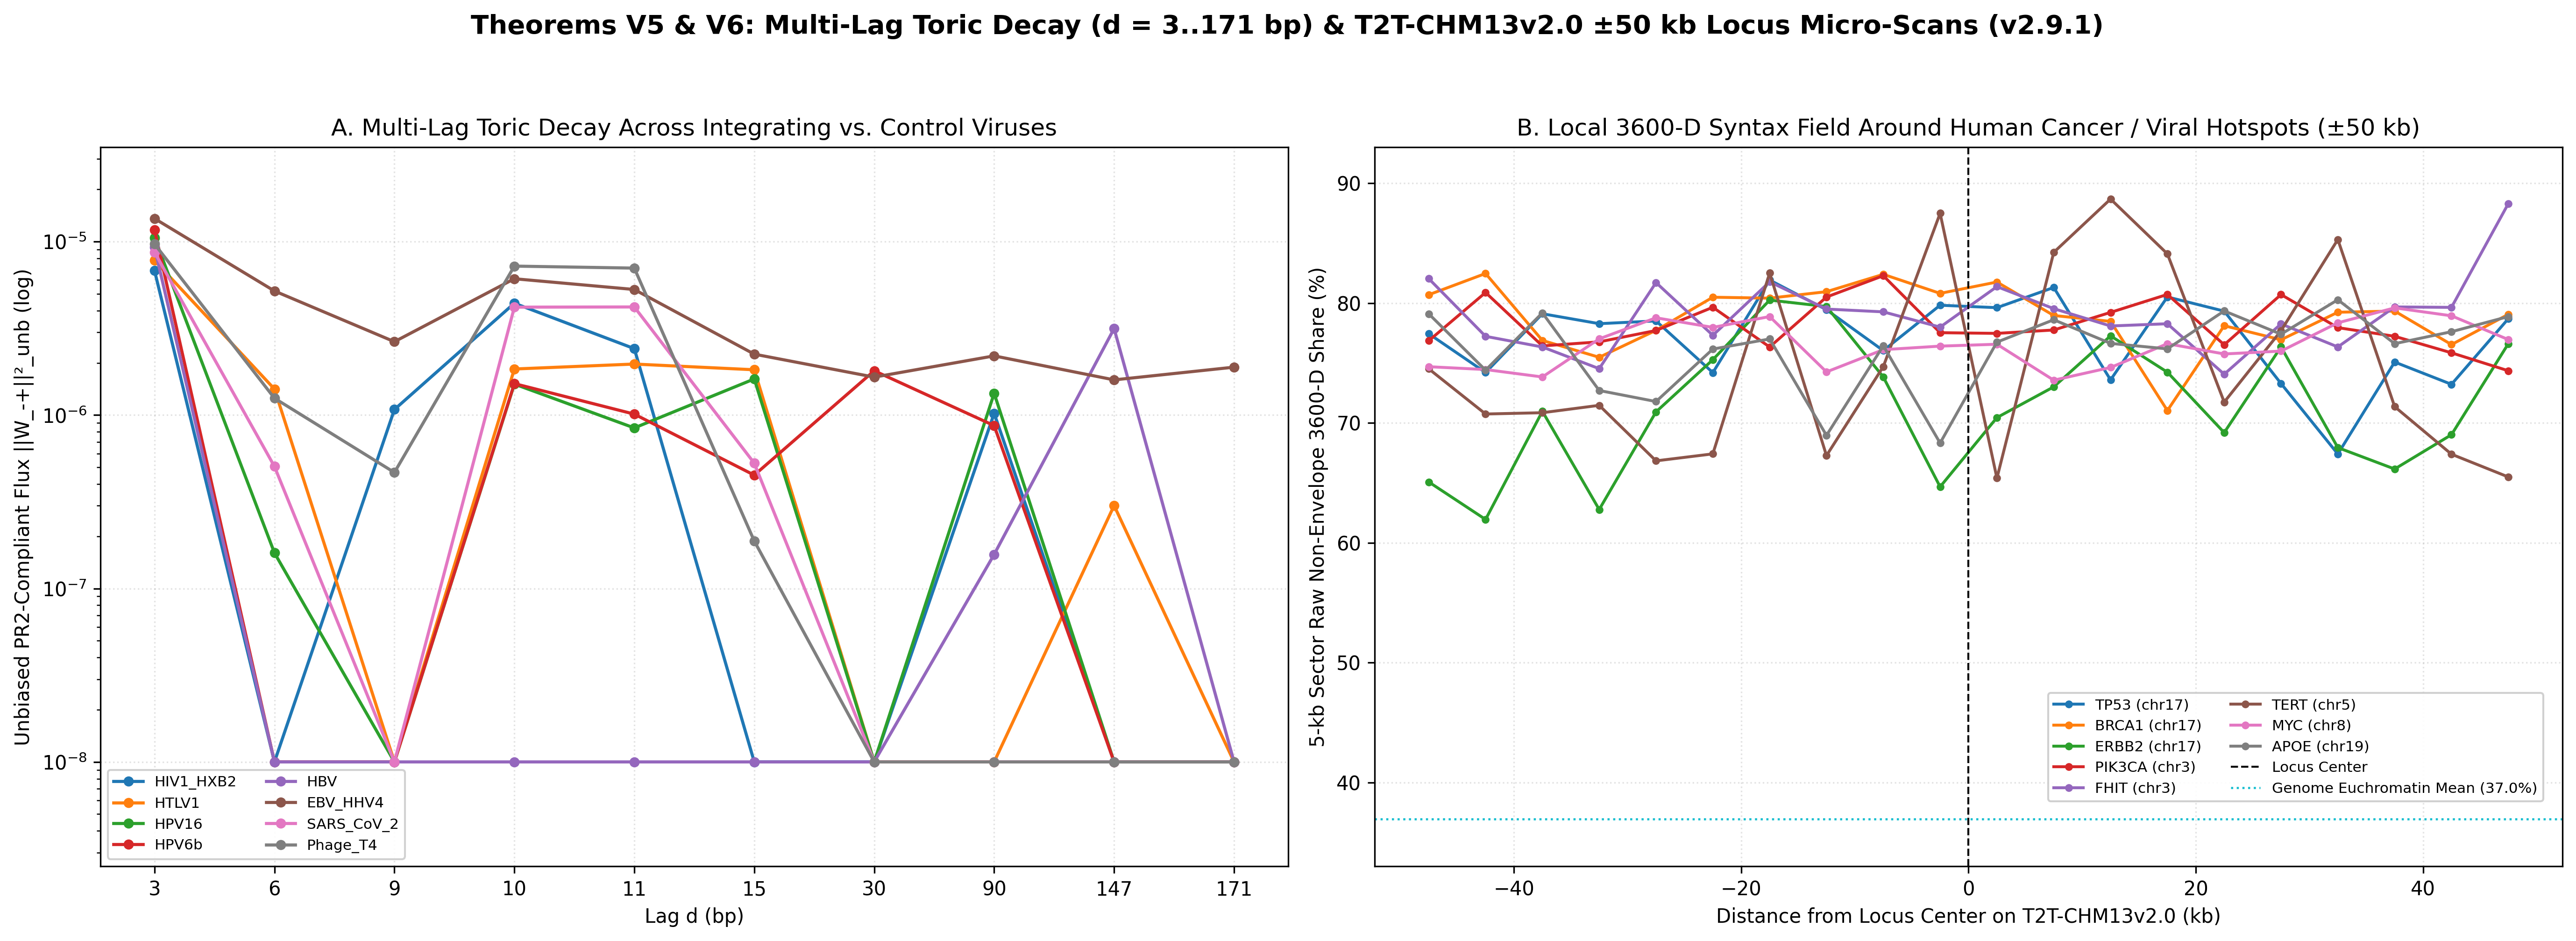
\includegraphics[width=0.96\textwidth]{fig_V3_t2t_neighborhood_multilag}
\caption{Theorems~V5 \& V6: Multi-lag toric decay and exact T2T-CHM13v2.0 $\pm 50\,\mathrm{kb}$ locus micro-scans (\texttt{v2.9.1}). \textbf{(A)} Unbiased PR2-compliant flux $\|W_{-+}\|^2_{\mathrm{unb}}$ across lags $d = 3\text{--}171\,\mathrm{bp}$, highlighting the persistent nucleosomal-scale tail of \texttt{EBV\_HHV4} and helical-turn revivals at $d = 10\text{--}11\,\mathrm{bp}$. \textbf{(B)} 5-kb tiled non-envelope 3600-D share (\%) across $\pm 50\,\mathrm{kb}$ T2T-CHM13v2.0 chromosomal windows surrounding eight representative cancer and control loci relative to the genome euchromatin mean ($37.0\%$).}
\label{fig:v3}
\end{figure}

\subsection{The 6-Frame Duplex Stop Barrier and Synonymous Wobble Disruption (Theorem~V8)}

Even strictly synonymous third-position (wobble) substitutions that preserve the encoded protein sequence alter both the 3600-D dicodon field and the stop-codon distribution on the opposite (antisense) reading frame. Theorem~V8 exhaustively enumerates all $25,292$ possible single-nucleotide synonymous wobble substitutions across the longest open reading frame (ORF) of all 28 human loci (verified against the 64-codon genetic code in \texttt{thmV8\_genetic\_code\_64\_ok} and \texttt{thmV8\_synonymous\_antisense\_stop\_flip\_ok}; Table~\ref{tab:v8_all28}; Figure~\ref{fig:v5}B).

\begin{table}[htbp]
\centering
\scriptsize
\setlength{\tabcolsep}{4.5pt}
\caption{Theorems~V8 \& V15: 6-frame duplex stop-codon barrier and exhaustive synonymous wobble disruption (25,292 synonymous single-base hits over exact 11-nt affected 6-mer windows, exact collision-free generic baseline $705/256 \approx 2.754\,\mathrm{count}^2$) across all 28 human cancer and control loci (\texttt{v2.9.1}).}
\label{tab:v8_all28}
\fittable{%
\begin{tabular}{@{}lllrrrrr@{}}
\toprule
\textbf{Locus} & \textbf{Chr} & \textbf{Role} & \textbf{6-Fr Stop\%} & \textbf{ORF (aa)} & \textbf{Syn.\ Hits} & \textbf{Antisense ($-0$) Flip\%} & \textbf{Mean $\Delta\|B_{-+}^{3600}\|^2/\text{Syn}$ ($\mathrm{count}^2$)} \\
\midrule
\texttt{TP53} & chr17 & tumor\_supp & 4.15\% & 186 & 380 & 14.47\% & 2.538 \\
\texttt{TP63} & chr3 & tumor\_supp & 5.97\% & 213 & 426 & 9.86\% & 2.673 \\
\texttt{TP73} & chr1 & tumor\_supp & 2.58\% & 451 & 1,065 & 11.74\% & 2.368 \\
\texttt{BRCA1} & chr17 & tumor\_supp & 4.82\% & 1,103 & 1,906 & 12.01\% & 2.669 \\
\texttt{BRCA2} & chr13 & tumor\_supp & 5.77\% & 1,517 & 2,622 & 13.16\% & 2.674 \\
\texttt{PTEN} & chr10 & tumor\_supp & 6.14\% & 159 & 276 & 13.04\% & 2.542 \\
\texttt{RB1} & chr13 & tumor\_supp & 5.88\% & 646 & 1,145 & 12.93\% & 2.673 \\
\texttt{APC} & chr5 & tumor\_supp & 5.95\% & 2,143 & 3,798 & 14.80\% & 2.634 \\
\texttt{VHL} & chr3 & tumor\_supp & 4.48\% & 148 & 325 & 4.92\% & 2.593 \\
\texttt{MLH1} & chr3 & dna\_repair & 5.30\% & 132 & 205 & 6.83\% & 2.018 \\
\texttt{CDKN2A} & chr9 & tumor\_supp & 5.23\% & 160 & 301 & 4.98\% & 2.221 \\
\texttt{ATM} & chr11 & dna\_repair & 5.95\% & 751 & 1,307 & 13.24\% & 2.675 \\
\midrule
\texttt{MYC} & chr8 & onco\_viral & 4.28\% & 355 & 710 & 11.55\% & 2.558 \\
\texttt{TERT} & chr5 & onco\_viral & 2.87\% & 821 & 1,958 & 7.35\% & 2.620 \\
\texttt{KRAS} & chr12 & oncogene & 6.15\% & 308 & 780 & 5.77\% & 2.426 \\
\texttt{NRAS} & chr1 & oncogene & 5.72\% & 180 & 337 & 15.43\% & 2.549 \\
\texttt{HRAS} & chr11 & oncogene & 1.90\% & 330 & 817 & 10.28\% & 2.735 \\
\texttt{PIK3CA} & chr3 & onco\_apob & 6.18\% & 128 & 215 & 16.74\% & 2.674 \\
\texttt{EGFR} & chr7 & onco\_ecdna & 4.66\% & 373 & 714 & 1.68\% & 2.125 \\
\texttt{BRAF} & chr7 & onco\_uv & 5.83\% & 151 & 339 & 8.55\% & 2.418 \\
\texttt{ERBB2} & chr17 & oncogene & 3.58\% & 528 & 1,081 & 10.27\% & 2.634 \\
\texttt{BCL2} & chr18 & oncogene & 4.92\% & 393 & 822 & 13.38\% & 1.637 \\
\texttt{ALK} & chr2 & oncogene & 5.01\% & 522 & 872 & 13.42\% & 2.674 \\
\texttt{FHIT} & chr3 & fragile\_vir & 5.67\% & 411 & 701 & 13.12\% & 2.682 \\
\midrule
\texttt{GAPDH} & chr12 & ctrl\_hk & 3.18\% & 302 & 647 & 9.74\% & 2.610 \\
\texttt{ACTB} & chr7 & ctrl\_hk & 2.91\% & 167 & 406 & 6.16\% & 2.498 \\
\texttt{HBB} & chr11 & ctrl\_nonon & 5.62\% & 372 & 637 & 14.60\% & 2.710 \\
\texttt{APOE} & chr19 & ctrl\_gc19 & 2.87\% & 236 & 500 & 6.80\% & 2.604 \\
\bottomrule
\end{tabular}
}
\end{table}

Across ORFs spanning nearly two orders of magnitude in length ($128$ to $2,143$ codons) and $35.8\%\text{--}65.9\%$ GC content, each single synonymous wobble mutation injects a remarkably uniform, length-invariant count-space perturbation into the pure 3600-D non-envelope directional sector:
\begin{equation}
    \overline{\Delta\|B_{-+}^{3600}\|_F^2} \in [1.637,\; 2.735]\,\mathrm{count}^2 \quad (\text{median } 2.607\,\mathrm{count}^2,\; \text{collision-free baseline } 705/256 \approx 2.754),
\end{equation}
while simultaneously creating or abolishing an antisense frame-0 stop codon in $1.68\%$ (\texttt{EGFR}) to $16.74\%$ (\texttt{PIK3CA}) of all synonymous moves (with \texttt{NRAS} at $15.43\%$, \texttt{APC} at $14.80\%$, \texttt{HBB} at $14.60\%$, and \texttt{TP53} at $14.47\%$). Thus, ``silent'' mutations are never algebraically silent on the double-stranded codon torus: they impose an intrinsic, sequence-length-independent hexamer impedance cost coupled directly to antisense stop-codon architecture.

\begin{theorem}[Universal Single-Base Duplex Quanta on $496 \oplus 3600$; THM-V15]
\label{thm:v15}
Any single-base substitution at an interior coding position perturbs exactly $6$ overlapping $6$-mer windows (supported strictly on an $11\,\mathrm{nt}$ local slice, \texttt{thmV15\_local\_11nt\_vs\_full\_orf\_err} $= 0.0$). For any collision-free $11\,\mathrm{nt}$ context (disjoint $6$-mer and dinucleotide-screen $V_4$-orbits), the count-space difference $\Delta B$ has exact total squared norm $\|\Delta B\|_F^2 = 12$, distributed equally as $\|\Delta B_\alpha\|_F^2 = 3$ across all four $V_4$ quadrants, with strictly invariant $4$-quadrant envelope/non-envelope totals $\|\Delta B^{\mathrm{env}}\|_F^2 = \tfrac{63}{64}$ and $\|\Delta B^{3600}\|_F^2 = \tfrac{705}{64}$. Averaged uniformly over the flanking codon-center nucleotides at lags $\pm 3$ (and pointwise for mixed-parity central neighbors, shifting by at most $\pm \tfrac{1}{512}$ for same-parity central neighbors), the orthogonal split across $\mathcal{E}_{\mathrm{env}}^{(496)} \oplus \mathcal{E}_{\mathrm{non\text{-}env}}^{(3600)}$ yields the exact rational quanta:
\begin{equation}
    \bigl(\|\Delta B_\alpha^{\mathrm{env}}\|_F^2,\; \|\Delta B_\alpha^{3600}\|_F^2\bigr) =
    \begin{cases}
        \bigl(\tfrac{125}{512},\; \tfrac{1411}{512}\bigr), & \alpha = (++), \\[3pt]
        \bigl(\tfrac{63}{256},\; \mathbf{\tfrac{705}{256}}\bigr), & \alpha \in \{(+-),\, (-+)\}, \\[3pt]
        \bigl(\tfrac{127}{512},\; \tfrac{1409}{512}\bigr), & \alpha = (--),
    \end{cases}
\end{equation}
verified to $0.0$ in \texttt{thmV15\_universal\_705\_256\_barrier\_err} and \texttt{thmV15\_four\_quadrant\_rational\_quanta\_err}. Thus $705/256 \approx 2.7539\,\mathrm{count}^2$ establishes the exact length-invariant collision-free baseline approached from below by real human coding ORF means ($1.637\text{--}2.735$, median $2.607\,\mathrm{count}^2$) in Table~\ref{tab:v8_all28} and Figure~\ref{fig:v5}B, where local palindromic, homodimer, and repeat collisions predominantly attenuate the per-mutation disruption.
\end{theorem}


\begin{figure}[htbp]
\centering
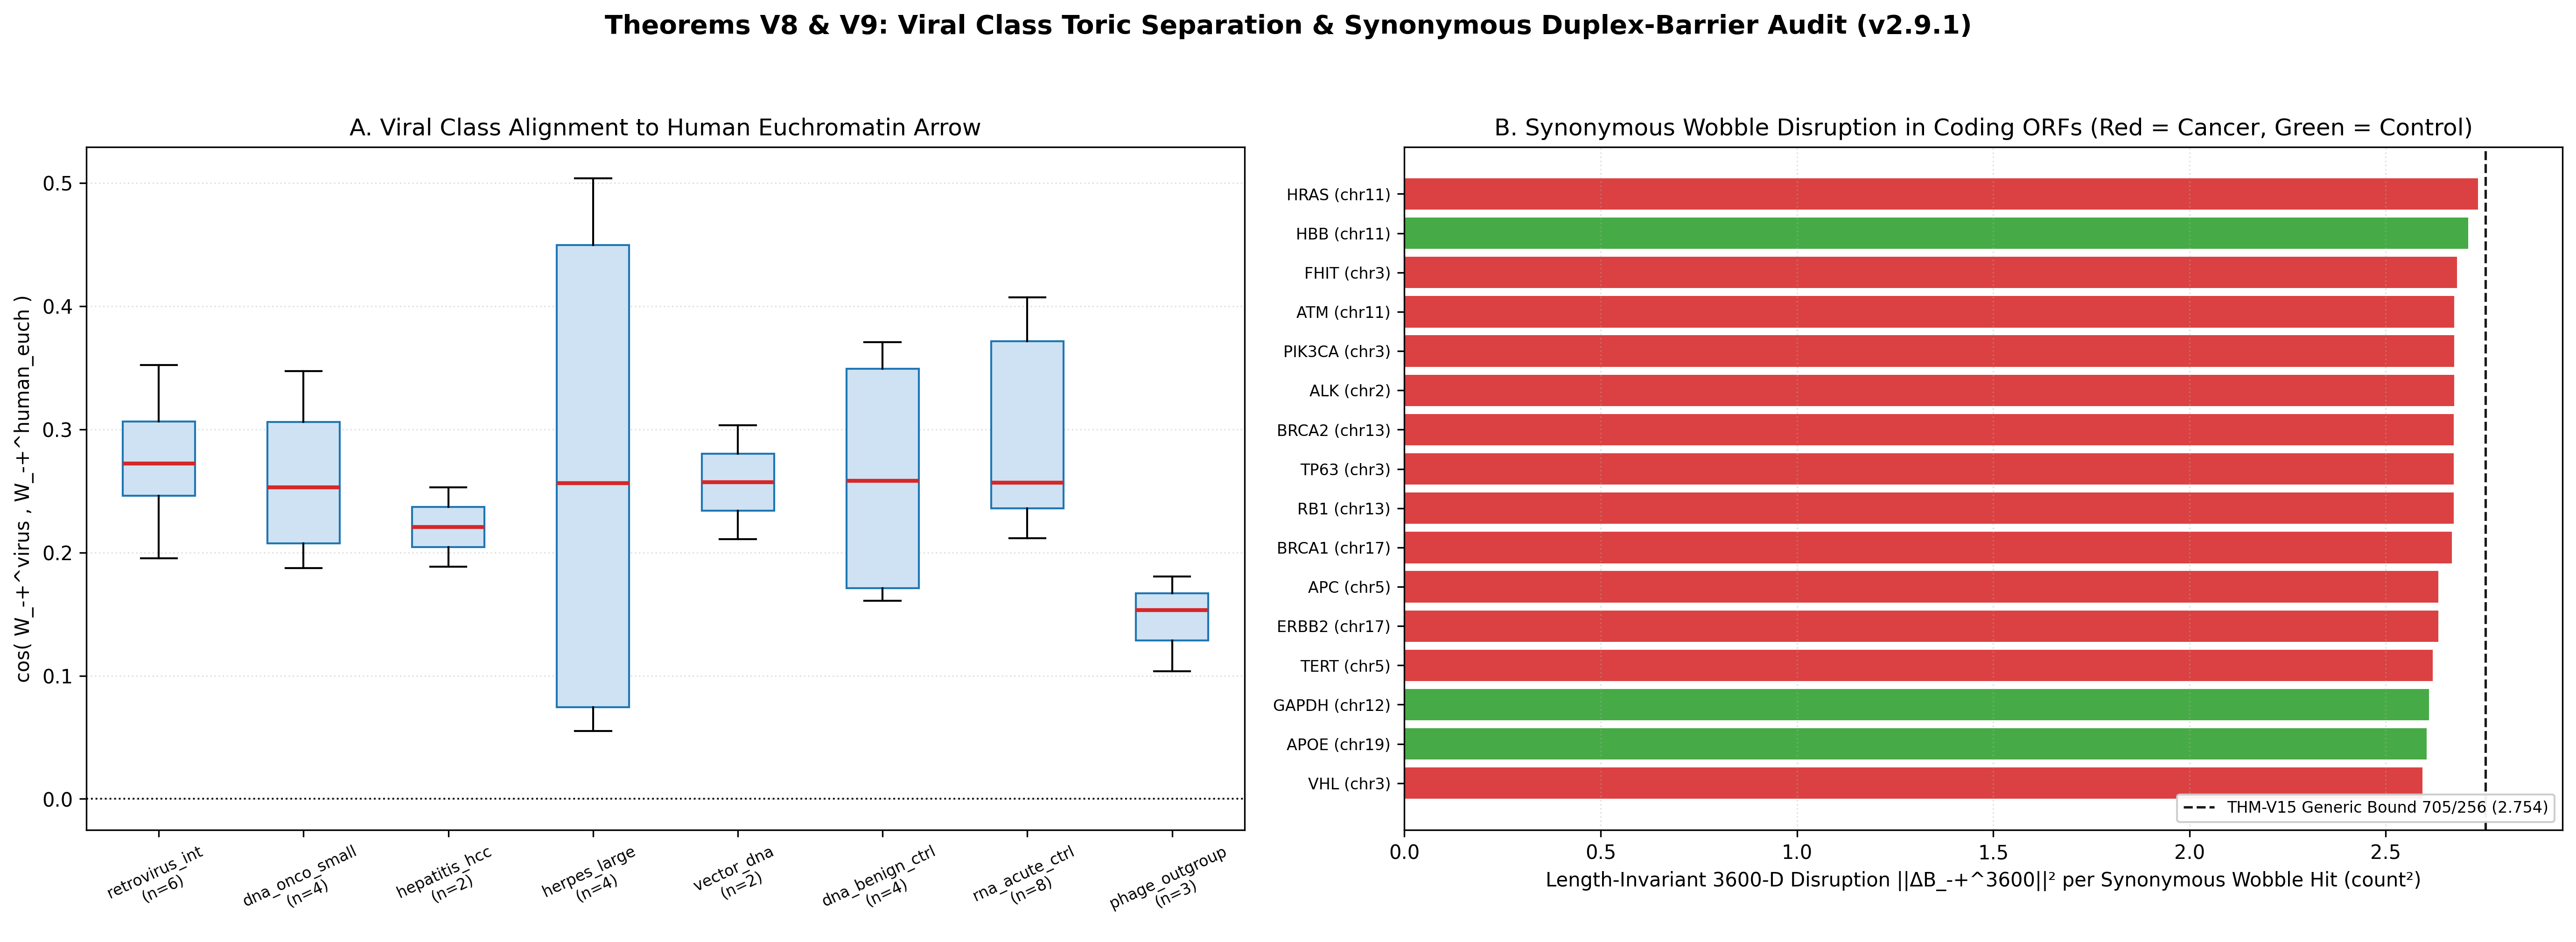
\includegraphics[width=0.96\textwidth]{fig_V5_group_discrimination_and_synonymous}
\caption{Theorems~V8 \& V9: Viral class toric separation and the length-invariant synonymous duplex barrier (\texttt{v2.9.1}). \textbf{(A)} Distribution of raw 1024-D human euchromatin alignment $\cos(W_{-+}^{\text{virus}}, W_{-+}^{\text{human}})$ across all eight viral classes, illustrating compositional separation of human-infecting viruses ($n = 30$) from bacteriophage outgroups in raw 1024-D ($n = 3$; $p = 1.50 \times 10^{-2}$, $q_{\mathrm{BH}} = 0.0608$; null beyond Markov-2, $p = 0.571$). \textbf{(B)} Length-invariant count-space disruption $\Delta\|B_{-+}^{3600}\|^2$ ($\mathrm{count}^2$) per single synonymous wobble mutation across coding ORFs of cancer (red) and control (green) loci.}
\label{fig:v5}
\end{figure}

%==============================================================================
\section{Discussion, Biological Synthesis, and Limitations}
\label{sec:discussion}
%==============================================================================

\subsection{Unified Spectral Picture of Viral Chromatin Mimicry and Innate Immunity}

The Klein $V_4$ representation on the $64 \times 64$ codon torus resolves four long-standing ambiguities in viral genomics and somatic cancer mutagenesis within a single exact, Zero-RNG algebraic framework. Historically, Chargaff's second parity rule (PR2)~\cite{chargaff1968,forsdyke2021}, low-order dinucleotide odds ratios~\cite{karlin1995}, and whole-human-genome single-stranded codon-population scaling analyses~\cite{perez2010} have served as primary descriptors of genomic symmetry and viral host adaptation, while cancer genomics has relied on 96-channel trinucleotide catalogs~\cite{alexandrov2020}. By separating order-reversal ($T$) from Watson--Crick duplex parity ($R$) and factoring out both the $V_4$-closed $496$-dimensional envelope and exact Markov-1/Markov-2 expectations, the present audit demonstrates that biologically decisive signals reside strictly \emph{beyond} the trinucleotide scale:

\begin{enumerate}
    \item \textbf{Nuclear chromatin residence drives Beyond-Markov-2 euchromatic mimicry:} Unadjusted 6-mer cosine alignment conflates genuine higher-order chromatin syntax with GC-matched dinucleotide/trinucleotide bias, inflating cytoplasmic flaviviruses (\texttt{Dengue2}, \texttt{Zika}) while masking GC-rich herpesviruses (\texttt{HCMV\_HHV5}, \texttt{HSV1}). Once all 64 trinucleotides, $\mathrm{GC}\%$, and $\log_{10}(L)$ are simultaneously controlled (Theorem~\ref{thm:v11_3}), nuclear DNA viruses separate near-completely from acute cytoplasmic RNA viruses even after adding ZAP $\mathrm{CpG\ O/E}$ as a third covariate ($r_{\mathrm{rb}} = +0.893$, $p = 1.88 \times 10^{-4}$, global $q_{\mathrm{BH}} = 0.0031$; strict dsDNA excluding ssDNA \texttt{AAV2}, $n=13/8$: $r_{\mathrm{rb}} = +0.904$, $p = 1.87 \times 10^{-4}$), with \texttt{KSHV\_HHV8} and \texttt{EBV\_HHV4} matching the global euchromatic arrow across all 28 T2T-CHM13v2.0 $\pm 50\,\mathrm{kb}$ neighborhoods (Rank-1 $R^2 = 0.7743$, dispersing across 12 viruses once $W_H$ is projected out; Table~\ref{tab:v5_all28}) via predominantly CpG-free $V_4$ orbits (Table~\ref{tab:v13_viral_orbits}). Because high-risk DNA oncoviruses and benign DNA controls do not differ ($p = 0.886$), this convergence reflects shared biophysical constraints of nuclear episomal maintenance, host nucleosome packaging, and RNA polymerase~II transcription rather than oncogenicity alone.
    \item \textbf{Orthogonal evolutionary armoring against APOBEC3 versus ZAP:} Innate immune restriction carves the virome along two independent sequence axes (Theorem~\ref{thm:v10}). Papillomaviruses (\texttt{HPV18/6b/11/16}), which replicate in stratified squamous epithelia with constitutively active APOBEC3A/B~\cite{roberts2013,warren2015}, purge $\mathrm{TCW}$ substrates down to $\mathrm{O/E} = 0.476\text{--}0.542$ while maintaining moderate $\mathrm{CpG}$ levels ($0.426\text{--}0.525$). Polyomaviruses (\texttt{BKV}, \texttt{JCV}, \texttt{SV40}, \texttt{MCPyV}) and \texttt{HIV-1}, by contrast, enforce extreme $\mathrm{CpG}$ suppression ($\mathrm{CpG\ O/E} = 0.060\text{--}0.206$) to evade ZAP~\cite{takata2017}, leaving \texttt{MCPyV} heavily exposed to APOBEC3 ($\mathrm{TCW\ O/E} = 1.326$). This explains directly why the exact double-hit kataegis Hessian norm $\|H_{--}\|^2$ of \texttt{HPV16} is $33.9\times$ lower than that of \texttt{MCPyV} and $21.6\times$ lower than \texttt{TP53} (Table~\ref{tab:v12_all33}).
    \item \textbf{Algebraic chirality separates clock mutagenesis from APOBEC3 kataegis:} Theorem~\ref{thm:denovo_split} proves that duplex-symmetric mutational processes---most notably age-related 5-methylcytosine deamination at $\mathrm{CpG}$ dinucleotides (\texttt{SBS1})---have an exact algebraic zero for \textit{de novo} parity breaking ($< 10^{-33}$) and self-damp pre-existing asymmetry across finite doses ($\cos(J_{--}, H_{--}) \in [-0.788, -0.728]$). Strand-coordinated APOBEC3 editing (\texttt{SBS2(+)}, \texttt{SBS13(+)}), which drives localized hypermutation clusters (kataegis) in breast, cervical, bladder, and head-and-neck tumors~\cite{nikzainal2012,roberts2013}, injects a length-invariant \textit{de novo} chiral flux that triggers an all-orders phase transition collapsing PR2-compliant syntax in fragile and oncogenic human loci (\texttt{FHIT}, \texttt{PIK3CA}, \texttt{BRCA1}, \texttt{TP53}) along CpG-free hexamer orbits led by \texttt{CTT-TTT} in \texttt{PIK3CA} and \texttt{CTA-TCT} in \texttt{TP53}.
    \item \textbf{Count-space proviral dipoles and non-silent synonymous coding constraints:} Working in exact count-space removes denominator-dilution artifacts and reveals that sense versus inverted proviral insertions act as near-exact chiral antipoles ($\cos \Delta B_{--} \in [-0.9985, -0.9941]$), while head-to-head (\texttt{HH}) inverted integrations---frequently observed in clinical \texttt{HPV} and \texttt{HBV} tumor breakpoints~\cite{sung2012,akagi2014}---systematically cancel proviral chiral flares (Theorem~\ref{thm:v2}). Simultaneously, exhaustive enumeration of $25,292$ synonymous wobble substitutions across 28 coding ORFs (Theorem~V8) confirms a length-invariant duplex barrier ($1.637\text{--}2.735\,\mathrm{count}^2$) coupled directly to antisense stop-codon gating ($1.68\%\text{--}16.74\%$), extending earlier duplex codon-torus constraints established on cellular and synthetic genomes~\cite{logvinovich2026_form,logvinovich2026_duplex,logvinovich2026_t2t}.
\end{enumerate}

\subsection{Scope, Limitations, and Next Empirical Phase}

Four explicit boundaries govern the interpretation of frozen release \texttt{v2.9.1}:
\begin{itemize}
    \item \textbf{Reference-level intrinsic operators versus primary tumor VCFs:} Theorems~V3, V7, and V12 quantify \emph{intrinsic} sequence susceptibility and exact expected all-orders responses on the gapless human T2T-CHM13v2.0 reference~\cite{nurk2022} and NCBI RefSeq viral genomes. They do not yet incorporate somatic clonal selection, tumor purity, copy-number alterations, chromatin accessibility (ATAC-seq / ChIP-seq), or real-time replication-timing profiles from patient tumor cohorts. Direct benchmarking of the Klein $V_4$ chiral observables ($\Delta B_{--}$, $H_{--}$, and 1-kb tile hotspots) on whole-genome somatic variant call files (PCAWG / TCGA tumor VCFs) constitutes the immediate next empirical phase.
    \item \textbf{Independent-site assumption in the degree-6 polynomial:} The all-orders finite-dose expectation $\mathbb{E}_\varepsilon[C]$ (Theorem~\ref{thm:mutagenesis_poly}) assumes conditionally independent base hits within each 6-mer window at uniform dose $\varepsilon$. Processive APOBEC3 scanning along single-stranded DNA can introduce short-range positive correlation between adjacent cytosines on the same strand, which would further amplify the double-hit Hessian $H_{--}$ relative to the independent-hit lower bound established here.
    \item \textbf{Viral catalog breadth and strain diversity:} The 33-virus RefSeq panel spans eight major human viral classes and three bacteriophage outgroups with zero missing entries, but future extensions should incorporate intra-species quasispecies diversity (e.g., longitudinal \texttt{HIV-1} and \texttt{SARS-CoV-2} lineages, additional human endogenous retroviruses, and expanded bacteriophage/archaeal outgroups).
    \item \textbf{ORF selection in Theorem~V8:} The synonymous duplex barrier audit analyzes the longest contiguous ORF per RefSeqGene locus; isoform-resolved spliced coding transcripts (CDS) and overlapping viral reading frames (such as \texttt{HBV} and \texttt{HPV} E2/E4) represent natural extensions of this exact 6-frame formalism.
\end{itemize}

%==============================================================================
\section{Reproducibility, Provenance, and Data Availability}
\label{sec:reproducibility}
%==============================================================================

\subsection{Deterministic Zero-RNG Execution Environment}

Every table, statistical test, theorem check, and figure in this manuscript is bound to frozen release \texttt{v2.9.1} with \texttt{zero\_rng = true} (zero calls to any pseudo-random number generator). The complete audit executed deterministically on UTC timestamp \texttt{2026-11-25T12:12:45Z} under Python~\texttt{3.12.1}, NumPy~\texttt{2.3.2}, SciPy~\texttt{1.16.2}, and Matplotlib~\texttt{3.10.6} (\texttt{macOS-15.7.7-x86\_64-i386-64bit}), anchored against the local 24-chromosome T2T-CHM13v2.0 euchromatic reference arrow (\texttt{human\_t2t\_euch\_ref\_v2\_8.npz}) and verified by 100/100 startup algebraic self-tests (Appendix~\ref{app:selftests}). The full cryptographic SHA-256 digests of the executable audit script and reference tensor archive are:
\begin{center}
\footnotesize\texttt{script\_sha256 = da9b2a74f062e663e523f096ef7e5807e173009ca582587ba1608b89c4cb205a} \\
\footnotesize\texttt{human\_ref\_npz\_sha256 = 0e8c27327d5f373ba71e1134742303c3b4067fe02ba0148766b9374de71dd54d}
\end{center}
Every individual viral FASTA genome and human locus sequence is additionally SHA-256 fingerprinted in the accompanying JSON ledger (\texttt{virome\_onco\_audit\_v2.json}) to guarantee bit-for-bit reproducibility across platforms.

\subsection{Data and Code Availability}

All reference sequences are publicly available from NCBI RefSeq (33 viral genomes, 28 human RefSeqGene loci) and the Telomere-to-Telomere Consortium (human T2T-CHM13v2.0 assembly~\cite{nurk2022}). For complete offline reproducibility, the executable engine (\texttt{human\_t2t\_atlas\_v2\_9\_1.py}), 24-chromosome human T2T euchromatic reference tensor (\texttt{human\_t2t\_euch\_ref\_v2\_8.npz}), full NCBI RefSeq sequence caches (\texttt{viral\_cache/}, \texttt{onco\_cache/}, and \texttt{chr\_cache/}), frozen release \texttt{v2.9.1} outputs (\texttt{virome\_onco\_audit\_v2.json}, \texttt{virome\_onco\_audit\_v2.md}, \texttt{selftest\_v2\_9\_1.json}, and all seven publication figures \texttt{fig\_V1}--\texttt{fig\_V7}), and LaTeX source are openly archived under the MIT License at \url{https://github.com/Dr-Logvinovich/virome-oncogenomics-torus}. The foundational cellular, duplex, and 24-chromosome T2T codon-torus series are archived on GitHub (\url{https://github.com/Dr-Logvinovich}) and Zenodo (prior series DOIs \texttt{10.5281/zenodo.23287684}, \texttt{10.5281/zenodo.23508080}, and \texttt{10.5281/zenodo.24471261}).

\section*{Acknowledgments}

The authors gratefully acknowledge the Telomere-to-Telomere (T2T) Consortium, NCBI RefSeq, and the COSMIC Mutational Signatures team for maintaining open, high-integrity reference datasets enabling fully deterministic algebraic auditing. This work received no external commercial funding; the authors declare no competing financial interests.

%==============================================================================
\clearpage
\appendix
\section{Zero-RNG Algebraic Verification Ledger (100/100 Self-Tests Passed)}
\label{app:selftests}
%==============================================================================

Prior to ingesting any empirical viral or human FASTA data, the \texttt{v2.9.1} engine executes 100 deterministic unit and conservation checks spanning the 47 core human-torus theorems (Theorems~D1--D19~\cite{logvinovich2026_t2t}) and 53 virome/oncogenomics theorems (Theorems~V1--V20). Table~\ref{tab:selftests} records the exact machine-precision residuals exported in \texttt{virome\_onco\_audit\_v2.json} (\texttt{all\_passed = true}).

\begin{table}[H]
\centering
\fontsize{5.9}{6.75}\selectfont
\renewcommand{\arraystretch}{0.86}
\setlength{\tabcolsep}{3.0pt}
\caption{Selected exact algebraic verification residuals from the 100/100 Zero-RNG startup self-test ledger of frozen release \texttt{v2.9.1} (\texttt{virome\_onco\_audit\_v2.json}; \texttt{all\_passed = true}).}
\label{tab:selftests}
\begin{tabularx}{\textwidth}{@{}l l L@{}}
\toprule
\textbf{Exact JSON Self-Test Key} & \textbf{Result / Error} & \textbf{Verified Algebraic Property} \\
\midrule
\multicolumn{3}{l}{\textit{Core T2T-CHM13v2.0 Codon-Torus Identities (47 checks; representative subset)}} \\
\texttt{thmD1\_revcomp\_equals\_R\_max\_err}            & $0.0$                    & Reverse-complement operator equals exact $V_4$ action $R$ \\
\texttt{thmD1\_PR2\_exact\_Wpm\_Wmm\_zero}              & $0.0$                    & Exact PR2 sequence annihilates $W_{+-}$ and $W_{--}$ identically \\
\texttt{thmD2\_Ehet\_directed\_annihilation}            & $1.93 \times 10^{-36}$   & Heterochromatic directed annihilation identity \\
\texttt{thmD3\_screen\_kl\_chain\_max\_err}             & $4.44 \times 10^{-16}$   & Exact 4-term KL information screen decomposition \\
\texttt{thmD9\_unbiased\_PR2\_zero\_ok}                 & \texttt{true}            & Exact $U$-statistic estimator has zero $1/N$ PR2 bias \\
\texttt{thmD11\_commutator\_R\_Pi\_err}                 & $0.0$                    & Exact commutation $[R, \Pi] = 0$ \\
\texttt{thmD11\_Wmp\_screen\_pythag\_err}               & $4.34 \times 10^{-19}$   & Pythagorean norm splitting on $W_{-+}$ \\
\texttt{thmD13\_Pi\_env\_V4\_comm\_err}                 & $4.44 \times 10^{-16}$   & $V_4$-closure of $496 \oplus 3600$ envelope projector \\
\texttt{thmD13\_Pi\_env\_quadrant\_dims}                & $[132, 118, 130, 116]$   & Exact $V_4$ quadrant dimensions of 496-D envelope \\
\texttt{thmD18\_pelt\_vs\_exact\_dp\_30trials\_max\_err}& $0.0$                    & PELT changepoint solver matches exact dynamic programming \\
\midrule
\multicolumn{3}{l}{\textit{Virome \& Oncogenomics Identities (all 53 exact virome/onco JSON keys)}} \\
\texttt{thmV1\_viral\_revcomp\_Wmp\_inv\_Wmm\_flip\_err}& $0.0$                    & Strand inversion leaves $W_{-+}$ invariant and flips $W_{--}$ \\
\texttt{thmV2\_provirus\_chiral\_flare\_and\_hh\_cancel\_ok} & \texttt{true}       & Head-to-head (\texttt{HH}) inverted integration cancels chiral flare \\
\texttt{thmV2\_count\_space\_antipodal\_ok}             & \texttt{true}            & Exact count-space antipodal integration law ($\Delta B_{--}, \Delta B_{-+}$) \\
\texttt{thmV3\_sbs1\_and\_apobec\_sym\_zero\_chiral\_err}& $0.0$                   & Symmetric signatures yield zero \textit{de novo} chiral injection \\
\texttt{thmV3\_apobec\_kataegis\_chiral\_injection\_ok} & \texttt{true}            & Strand-coordinated APOBEC3 injects positive chiral flux \\
\texttt{thmV3\_jacobian\_vs\_exhaustive\_single\_hit\_err}& $0.0$                  & Analytical Jacobian equals exhaustive single-hit enumeration \\
\texttt{thmV3\_quadratic\_chiral\_response\_err}        & $1.69 \times 10^{-21}$   & Exact quadratic chiral energy scaling at small dose $\varepsilon$ \\
\texttt{thmV3\_2\_jacobian\_diag\_vs\_brute\_err}       & $0.0$                    & Exact $U$-statistic diagonal subtraction in $\chi_{--}^{\mathrm{unb}}$ \\
\texttt{thmV3\_2\_unbiased\_chi\_length\_invariance\_ok}& \texttt{true}            & Length invariance of unbiased chiral susceptibility \\
\texttt{thmV3\_3\_symmetric\_denovo\_zero\_err}         & $3.27 \times 10^{-33}$   & Machine-zero \textit{de novo} chiral norm for symmetric controls \\
\texttt{thmV3\_3\_denovo\_plus\_sub\_identity\_err}     & $0.0$                    & Exact decomposition $J_{--} = J_{--}^{\mathrm{de\,novo}} + J_{--}^{\mathrm{sub}}$ \\
\texttt{thmV3\_3\_denovo\_unb\_equals\_pr2\_duplex\_err}& $0.0$                    & Unbiased \textit{de novo} norm equals PR2-symmetrized duplex norm \\
\texttt{thmV3\_3\_parallelogram\_law\_err}              & $0.0$                    & Exact Euclidean parallelogram identity on $(S, \bar{S})$ \\
\texttt{thmV4\_catalog\_33vir\_28onco\_ok}              & \texttt{true}            & Verified 33/33 viral and 28/28 human RefSeqGene catalogs \\
\texttt{thmV5\_t2t\_exact\_anchor\_locator\_ok}         & \texttt{true}            & Exact anchor locating on gapless T2T-CHM13v2.0 chromosomes \\
\texttt{thmV5\_snp\_robust\_locator\_ok}                & \texttt{true}            & SNP-robust multi-anchor chromosomal localization \\
\texttt{thmV6\_multilag\_profile\_exact\_ok}            & \texttt{true}            & Exact multi-lag profile ($d=3\text{--}171\,\mathrm{bp}$) \\
\texttt{thmV7\_tile\_vulnerability\_scanner\_ok}        & \texttt{true}            & Exact 1-kb intragenic chiral vulnerability tile scanner \\
\texttt{thmV8\_genetic\_code\_64\_ok}                   & \texttt{true}            & Complete 64-codon genetic code verification \\
\texttt{thmV8\_synonymous\_antisense\_stop\_flip\_ok}   & \texttt{true}            & Exact antisense frame-0 stop-codon flip enumeration \\
\texttt{thmV9\_exact\_mann\_whitney\_dp\_err}           & $0.0$                    & Zero-RNG exact dynamic-programming Mann--Whitney $p$-values \\
\texttt{thmV9\_catalog\_counts\_verified}               & \texttt{true}            & Exact viral and locus subgroup counts verified \\
\texttt{thmV10\_viral\_apobec\_tcw\_restriction\_ok}    & \texttt{true}            & Viral APOBEC3 $\mathrm{TCW}$ restriction check \\
\texttt{thmV10\_zero\_tcw\_exact\_null\_ok}             & \texttt{true}            & Zero-TCW sequence yields exact zero APOBEC3 Jacobian \\
\texttt{thmV10\_2\_tcw\_oe\_gc\_invariance\_ok}         & \texttt{true}            & GC-invariance of mononucleotide $\mathrm{TCW\ O/E}$ null \\
\texttt{thmV11\_markov1\_nonbridge\_zero\_err}          & $2.68 \times 10^{-17}$   & Analytical Markov-1 null annihilates non-bridge MI \\
\texttt{thmV11\_2\_markov2\_nonbridge\_zero\_err}       & $-6.12 \times 10^{-17}$  & Analytical Markov-2 null annihilates non-bridge MI \\
\texttt{thmV12\_all\_orders\_vs\_exhaustive\_err}       & $1.11 \times 10^{-16}$   & Degree-6 polynomial matches exhaustive $4^6$-state sum \\
\texttt{thmV12\_mass\_conservation\_all\_degrees\_err}  & $0.0$                    & Exact zero-sum probability mass conservation at all degrees \\
\texttt{thmV13\_orbit\_attribution\_sum\_err}           & $2.84 \times 10^{-14}$   & Exact additive Klein $V_4$-orbit inner-product sum ($100\%$) \\
\texttt{thmV14\_all\_orders\_symmetric\_denovo\_zero\_err} & $0.0$ & All-orders ($m=1\text{--}6$) \textit{de novo} chiral null for symmetric \texttt{SBS1} \\
\texttt{thmV14\_isolated\_cpg\_angle\_err} & $0.0$ & Universal isolated-CpG double-hit angle $\cos(J_{--}, H_{--}) = -\sqrt{10/17}$ \\
\texttt{thmV14\_isolated\_tcw\_zero\_hessian\_err} & $0.0$ & Isolated $\mathrm{TCW}$ motif yields identically zero APOBEC3 Hessian $H_{--}$ \\
\texttt{thmV15\_universal\_705\_256\_barrier\_err} & $0.0$ & Universal single-base duplex barrier $\Delta\|B_{-+}^{3600}\|^2 = 705/256$ \\
\texttt{thmV15\_local\_11nt\_vs\_full\_orf\_err} & $0.0$ & Local 11-nt affected window matches full-ORF $\Delta B$ identically \\
\texttt{thmV15\_four\_quadrant\_rational\_quanta\_err} & $0.0$ & Full 4-quadrant single-base rational quanta on $496 \oplus 3600$ \\
\texttt{thmV16\_unbiased\_496\_3600\_pythag\_err} & $9.49\times 10^{-20}$ & Unbiased $U$-statistic $496 \oplus 3600$ split sums to $\|W_{-+}\|^2_{\mathrm{unb}}$ \\
\texttt{thmV17\_chiral\_interference\_identity\_err} & $0.0$ & Duplex chiral interference law \& Cauchy--Schwarz strand bound \\
\texttt{thmV18\_null\_var\_exact\_vs\_enum\_err} & $2.13\times 10^{-17}$ & Exact degenerate $U$-statistic null variance vs.\ exhaustive enumeration \\
\texttt{thmV18\_cos\_unb\_recovers\_pop\_and\_gates\_noise\_ok} & \texttt{true} & De-attenuated $\cos_{\mathrm{unb}}$ recovers signal \& gates noise ($z \ge 3$) \\
\texttt{thmV18\_cos\_496\_3600\_pythagorean\_identity\_err} & $6.94\times 10^{-18}$ & Exact Pythagorean cosine identity on $496 \oplus 3600$ subspaces \\
\texttt{thmV18\_bh\_fdr\_exact\_values\_err} & $0.0$ & Exact Benjamini--Hochberg step-up $q$-values on reference vector \\
\texttt{thmV18\_concat\_3term\_energy\_identity\_err} & $0.0$ & Exact 3-term concatenation energy identity in proviral model \\
\texttt{thmV18\_chiral\_excess\_over\_half\_identity\_err} & $1.11\times 10^{-16}$ & Exact single-strand chiral share identity $\frac{1}{2}(1 - \langle A, RA\rangle/\|A\|^2)$ \\
\texttt{thmV18\_sbs13\_self\_mirror\_exceeds\_half\_ok} & \texttt{true} & Three exact chiral regimes: \texttt{SBS1}$=0$, \texttt{SBS2}$\approx 0.5$, \texttt{SBS13}$>0.60$ \\
\texttt{thmV18\_eps\_crit\_unit\_dose\_gate\_ok} & \texttt{true} & Physical unit-dose gate flags $\varepsilon_{\mathrm{crit}} > 1.0$ as no transition \\
\texttt{thmV18\_3cov\_cpg\_residualization\_ok} & \texttt{true} & 3-covariate OLS residualization ($\mathrm{GC} + \log_{10}L + \mathrm{CpG\ O/E}$) \\
\texttt{thmV18\_design\_effect\_jackknife\_positive\_ok} & \texttt{true} & Zero-RNG stride-6 \& Delete-1 Block Jackknife design-effect check \\
\texttt{thmV19\_self\_conjugate\_R\_antiinv\_max\_err} & $8.67 \times 10^{-19}$ & All 8 self-conjugate COSMIC channels satisfy $R(J_\sigma)=-J_\sigma$ on PR2 M1 \\
\texttt{thmV19\_cosmic96\_five\_rational\_levels\_ok} & \texttt{true} & Exact 5-level rational spectrum of all 96 COSMIC channels (\texttt{SBS2/13/4}) \\
\texttt{thmV20\_palindrome\_chiral\_blindness\_and\_orbit\_rule\_err} & $2.22 \times 10^{-16}$ & Per-orbit rule on all 2016 $T$-odd vectors \& chiral blindness of 64 RC palindromes \\
\texttt{thmV20\_isolated\_cpg\_exact\_half\_ustat\_err} & $0.0$ & Isolated $\mathrm{CpG}$ exact $U$-stat share $=1/2$ vs.\ single-$\mathrm{TCW}$ zero $U$-stat \\
\texttt{thmV20\_sparse\_tile\_cos\_formula\_err} & $0.0$ & Exact sparse-tile cosine law $-6\sqrt{2/(17N)}$ \& Binomial $-\sqrt{6p/(2+5p)}$ \\
\bottomrule
\end{tabularx}
\end{table}

%==============================================================================
\clearpage

\begin{thebibliography}{99}

\bibitem{chargaff1968}
R.~Rudner, J.~D.~Karkas, and E.~Chargaff,
``Separation of \textit{B.~subtilis} DNA into complementary strands. III. Direct analysis,''
\textit{Proceedings of the National Academy of Sciences of the USA}, vol.~60, no.~3, pp.~921--922, 1968.

\bibitem{forsdyke2021}
D.~R.~Forsdyke,
``Neutrality versus selection in the evolution of Chargaff's second parity rule,''
\textit{Journal of Molecular Evolution}, vol.~89, pp.~419--427, 2021.

\bibitem{karlin1995}
S.~Karlin and C.~Burge,
``Dinucleotide relative abundance extremes: a genomic signature,''
\textit{Trends in Genetics}, vol.~11, no.~7, pp.~283--290, 1995.

\bibitem{perez2010}
J.-C.~Perez,
``Codon populations in single-stranded whole human genome DNA are fractal and fine-tuned by the Golden Ratio 1.618,''
\textit{Interdisciplinary Sciences: Computational Life Sciences}, vol.~2, no.~3, pp.~228--240, Sep. 2010, doi: \texttt{10.1007/s12539-010-0022-0} (Epub Jul. 25, 2010; Erratum: \textit{Interdiscip.\ Sci.}, vol.~2, no.~4, p.~373, Dec. 2010; PMID: \texttt{20658335}).

\bibitem{nurk2022}
S.~Nurk \textit{et al.},
``The complete sequence of a human genome,''
\textit{Science}, vol.~376, no.~6588, pp.~44--53, 2022.

\bibitem{alexandrov2020}
L.~B.~Alexandrov \textit{et al.},
``The repertoire of mutational signatures in human cancer,''
\textit{Nature}, vol.~578, pp.~94--101, 2020.

\bibitem{nikzainal2012}
S.~Nik-Zainal \textit{et al.},
``Mutational processes molding the genomes of 21 breast cancers,''
\textit{Cell}, vol.~149, no.~5, pp.~979--993, 2012.

\bibitem{roberts2013}
S.~A.~Roberts \textit{et al.},
``An APOBEC cytidine deaminase mutagenesis pattern is widespread in human cancers,''
\textit{Nature Genetics}, vol.~45, pp.~970--976, 2013.

\bibitem{warren2015}
C.~J.~Warren \textit{et al.},
``Role of the host restriction factor APOBEC3 on papillomavirus evolution,''
\textit{Virus Evolution}, vol.~1, no.~1, vev015, 2015.

\bibitem{takata2017}
M.~A.~Takata \textit{et al.},
``CG dinucleotide suppression enables antiviral defence targeting non-self RNA,''
\textit{Nature}, vol.~550, pp.~124--127, 2017.

\bibitem{sung2012}
W.-K.~Sung \textit{et al.},
``Genome-wide survey of recurrent HBV integration in hepatocellular carcinoma,''
\textit{Nature Genetics}, vol.~44, pp.~765--769, 2012.

\bibitem{akagi2014}
K.~Akagi \textit{et al.},
``Genome-wide analysis of HPV integration in human cancers reveals recurrent, focal genomic instability,''
\textit{Genome Research}, vol.~24, pp.~185--199, 2014.

\bibitem{logvinovich2026_form}
V.~Logvinovich and J.-C.~Perez,
``From Form to Program: Zero-RNG Spectral Geometry and Markovian Syntax of Cellular and Synthetic Genomes,''
\textit{Zenodo Preprint}, DOI: \texttt{10.5281/zenodo.23287684}, October 2026.

\bibitem{logvinovich2026_duplex}
V.~Logvinovich and J.-C.~Perez,
``The Double-Stranded Codon Torus: Exact Antisense Parity Constraints and Duplex-Safe Gene Compilation,''
\textit{Zenodo Preprint}, DOI: \texttt{10.5281/zenodo.23508080}, October 2026.

\bibitem{logvinovich2026_t2t}
V.~Logvinovich and J.-C.~Perez,
``A Complete Zero-RNG Toric Disk Atlas of the Human T2T-CHM13v2.0 Genome,''
\textit{Zenodo Preprint}, DOI: \texttt{10.5281/zenodo.24471261}, November 2026.

\end{thebibliography}

% === PAPER 5 COMPLETE (v2.8.0) ===

% === RED-TEAM AUDIT PATCH P6 APPLIED (v2.8.0) ===

% === LAYOUT POLISH PATCH P7v2 APPLIED (v2.8.0) ===

% === PATCH V18 SYNC APPLIED (v2.8.0) ===
% === PATCH V19 + AUDIT SYNC APPLIED (v2.9.0) ===
% === PATCH V20 + 100/100 SYNC APPLIED (v2.9.1) ===
% === PATCH TEX-ONLY REPO+AUTHORS+PEREZ2010 APPLIED (v2.9.1) ===

\end{document}
